\documentclass{article}
\usepackage[utf8]{inputenc}
\usepackage{pifont}
\usepackage{fullpage}
\usepackage{graphicx}
\usepackage{subcaption}
\usepackage{caption}
\usepackage{comment}
\usepackage{titletoc}
\usepackage{titlesec}
\usepackage{color}
\usepackage{todonotes}
\usepackage{amsmath}
\usepackage{amssymb}
\usepackage{multirow}
\usepackage[final]{microtype} % better folding

\usepackage[backend=biber,style=nature,sorting=ynt]{biblatex}
\addbibresource{migration-paper.bib}

% \newcommand{\SMC}{SMCSMC }

\title{Ancient Admixture into Africa from the ancestors of non-Africans}
% Directional Migration into Africa in the Late Middle Paleolithic
\author{Christopher B. Cole, Sha Joe Zhu, Iain Mathieson, Kay Pr\"ufer, Gerton Lunter}
\date{}

\begin{document}
\maketitle
% do not add main paper to supplementary TOC
\addtocontents{toc}{\protect\setcounter{tocdepth}{0}}

%
% TODO (GL 27/3/2020)
%
% - We refer to San, KhoeSan, Khomani San, Khoesan.  I'm a bit lost here.  Ideally we use fewer ways to refer to these population(s), and explain how these terms are related v briefly somewhere.
% -Rationalize citations for methods.  Fewer ARG-based references,
%  add a few key references for site-frequency-spectrum based methods
% - Add citations SGDP, HGDP
% - Use RCCR throughout (e.g. y-axis of Fig 1c,d)
% - Include definition of IMF (direction, epoch) in caption of Table S1
%             (*) Use eithter "Khomani San" (in legend above B) or "Khoesan"
%                 (axis panel H) but not both - or am I missing something? 
%                    - Khoesan refer to both Ju Hoan and Khomani San; Khomani refers to one group
%             (*) Make lettering a bit bigger (x)
% - Figure 2: (*) Use lower-case and boldface labels A-E. (x)
%             (*) Make lettering a bit bigger (x)
%             (*) Panels C-E, use more contrasting colour for Inferred Single
%                 African, perhaps dark green?  Or dotted black, to make similar
%                 to panel B?
%             (*) Make panels C D E slightly taller (not wider) to 
%                 match aspect ratio (fixed ratio at 1 for mig plots, 9/16 for Ne)
% - (x) Redo segment computation and analyses that depend on it, using 40-70 kya epoch (done)
% - Section S2.1 and Fig S11.  
%   - Include inferred slope of Fig S11b to the caption of S11 or text S2.1.
%   - Text S2.1:  "...is well approximated by (rT)^-1 [42]; ..."  The formula misses
%     a factor (1-m).
%       - (cc) this is actually from the text, though I've included the extra term for our purposes. 
%   - Mention in text S2.1 that the slope of the log histogram S11b, not the mean,
%     is the best estimator for the 1/(1-m)rT parameter, because very short segments will
%     tend to be missed by SMCSMC, as can be seen from the empirical histogram (and
%     this is the bin with the largest number of segments by far)
%        - (cc) Sorry, I'll come back to this, I'm not sure that I understand
%   - Explain what the yellow area is in S11a. (cc done)
%   - Switch S11a / S11b in the caption to S11 (cc done)
%   - Add small symbols (filled circles?) to S11b -- this really should be a histogram,
%     not a line graph, but doing multiple histograms will clutter this up.
%   - Explain in the caption what the bin size is for the histogram S11b.
%   - S11a: x axis is not migration rate per generation -- is it IMF (and if so, mention
%     the epoch over which it was integrated), or did you miss a 10^-X scale factor?
%
% Additional analyses, for after submission
%
% - Run analysis of Fig. 3 for more iterations (15), and more particles (10k), and
%   with proportion replaced 0 / 0.1 / 0.2 / 0.3 / 0.4 / 0.5 / 0.6 (to get better 
%   resolved FW and BW estimates particularly for the true BW migration case)

\begin{abstract}
\noindent Genetic diversity across human populations has been shaped by demographic history, making it possible to infer past demographic events from extant genomes. However, demographic inference in the ancient past is difficult, particularly around the out-of-Africa event in the Late Middle Paleolithic, a period of profound importance to our species' history.  Here we present {\tt SMCSMC}, a Bayesian method for inference of time-varying population sizes and directional migration rates under the coalescent-with-recombination model, to study ancient demographic events. We find evidence for substantial migration from the ancestors of present-day Eurasians into African groups between 40 and 70 thousand years ago, predating the divergence of Eastern and Western Eurasian lineages.  This event accounts for previously unexplained genetic diversity in African populations, and supports the existence of novel population substructure in the Late Middle Paleolithic. Our results indicate that our species' demographic history around the out-of-Africa event is more complex than previously appreciated.
\end{abstract}

\section{Introduction}

Methods to characterize demographic history from genetic data alone form a useful and independent complement to archaeological approaches \cite{Nielsen2017a}, and many methods have been developed for this purpose \cite{Li2011,Pickrell2012,Rasmussen2014,Schiffels2014a,Mathieson2014,Steinrucken2015,Malaspinas2016,Chikhi2018,Speidel2019,Kelleher2019,Wang2019a,Albers2019}. These methods are particularly useful for making inference about human history at the end of the Middle Paleolithic approximately 60 thousand years ago (kya). This period saw the divergence of the most deeply sampled lineages of human genetic variation, introgression from multiple archaic sources, and the expansion of anatomically modern humans out of Africa (OoA). However, due to the relative scarcity of archaeological evidence and ancient DNA in this period, demographic inference has the potential to be very informative, though technically challenging.

The phylogenetic trees over a set of samples as they change along the genome through recombination, collectively referred to as the ancestral recombination graph (ARG) \cite{Griffiths1997a,Rasmussen2014}, record all information about the samples' evolutionary history.  This history itself is shaped by the population's demography, a statistical relationship that is quantified by the coalescent-with-recombination (CwR) model \cite{Griffiths1997a}.  The ARG is a complex data structure and is only weakly constrained by the observed genetic polymorphisms, making inference of demography difficult. By making approximations to the CwR, for instance by making an independent-sites assumption, efficient parametric inference of demography becomes possible \cite{Excoffier2013,McVean2005}.  Methods including {\tt PSMC} \cite{Li2011}, {\tt diCal} \cite{Steinrucken2015} and {\tt SMC++} \cite{Terhorst2015} allow non-parametric inference of demography under a closer approximation to the CwR, but one that does not include gene flow between populations. {\tt MSMC} \cite{Schiffels2014} introduced the cross-coalescent rate and {\tt MSMC-IM} described how to interpret this rate in the context of a isolation-migration model to estimate a migration rate between populations\cite{Wang2019a}. However, these methods are not well suited for estimating directional migration rates.

Here we extend {\tt SMCSMC} (Sequential Monte Carlo inference of the Sequentially Markovian Coalescent, \cite{Henderson2018}) to allow inference of directional migration.  {\tt SMCSMC} is a Bayesian method that uses a particle filter to explicitly sample from the posterior distribution of ARGs over multiple diploid samples under the full CwR model.
Since particle filters operate by simulating latent variables (here the ARG) under the statistical model of interest, it becomes possible to handle complex demographic scenarios.  We exploit this by extending the CwR model to include time-varying directional migration rates in a two-island demographic model.  We use the posterior sample of ARGs including migration events to update the parameters of the demographic model, using either expectation-maximization or a variational Bayes procedure, and iterate these steps until convergence.   We apply {\tt SMCSMC} to estimate directional migration rates in whole genome sequencing data from the Simons Genome Diversity Panel (SGDP) \cite{Mallick2016} and the Human Genome Diversity Panel (HGDP) \cite{Bergstrom2019} to investigate population structure around the OoA event.

\section{Results}

\paragraph{Substantial Migration from Eurasian to African Ancestors} We use {\tt SMCSMC} to analyse pairs of individuals from the SGDP and simultaneously infer migration rates and effective population sizes ($N_e$) under a two-island model with directional migration.  Population sizes and migration rates are modeled as piece-wise constant across 32 exponentially spaced epochs from 133 to 133016 generations in the past, corresponding to 3.8 thousand to 3.8 million years ago (3.8kya--3.8Mya) using a generation time $g=29$ years \cite{Fenner2005}.  We find that the method infers high rates of migration from descendants of the OoA event ('non-Africans') to Africans, but not in the opposite direction, in the period $30$--$70$kya corresponding to the Late Middle Paleolithic (Fig.\ \ref{migrationplot}). In populations from the Niger-Kordofanian and Nilo-Saharan language groups, comprising the majority of the population on the African continent, the peak inferred migration rate from Eurasian populations ($2.5$--$3.0\times 10^{-4}$ and $3.5$--$4.0\times 10^{-4}$, in units of proportion of the target (ancestral African) population replaced per generation) most frequently falls in the epochs spanning 35--45kya, while peak migration rates in the opposite direction are substantially lower ($0.5$-$1.0\times 10^{-4}$) and occur earlier, in the epochs spanning $55$--$70$kya (Supplemental Fig.\ \ref{fig:peaks}). Populations in the Afroasiatic language group show evidence of large amounts of directional migration in the Holocene (Supplemental Fig.\ \ref{sgdp_mig}), which is consistent with previous findings of relatively recent European introgression into these populations \cite{Busby2016, Fan2019}. 

To assess the impact of errors introduced by statistical phasing, which was used to phase the SGDP samples, we repeated the analyses above on a subset of physically phased individuals from the Human Genome Diversity Project (HGDP) \cite{Mallick2016} (Supplemental Section \ref{hgdp_section}). This data set comprises individuals from four African (Yoruban, San, Mbuti, and Biaka) and nine non-African populations (Druze, Han, Karitiana, two Papuan populations, Pathan, Pima, Sardinian, and Yakut). {\tt SMCSMC} results in the HGDP are qualitatively similar to those in the SGDP (Fig.\ \ref{migrationplot}b, Supplemental Fig.\ \ref{fig:peaks}a). Inferred migration rates are, in general, lower in HGDP data than when using matched SGDP samples (Figs.\ \ref{migrationplot}a,b and \ref{fig:both}, demographic inference in matched sampled in Supplemental Figure \ref{fig:hgdp_sgdp}), but in all cases, the migration rates from Eurasia to Africa are substantially higher than in the opposite direction, consistent with the findings in the SGDP (Supplemental Fig.\ \ref{fig:both}). 

We asked whether {\tt SMCSMC} has power to detect a large back-migration event in the Late Middle Paleolithic and distinguish it from other demographic scenarios. To answer this we used {\tt SCRM} \cite{Staab2015} to simulate a gigabase of sequence data under a two-island demographic model,
%with a split time of 385kya, 
and effective population sizes chosen to be comparable to typical African and Eurasian populations as inferred from real data. 
%We simulated an early split time to allow {\tt SMCSMC} to resolve the split times of the populations without undue bias. \textcolor{red}{\bf This explanation sounds weak.  It suggests that we're making simulating an easier case than reality, throwing doubt on our simulations.  Thoughts?} 
To this we added a $10$ky pulse of forward, backward or bidirectional migration of varying strengths, with the midpoint of the migration pulse within the range $40$ to $70$kya.  To quantify the inferred amount of migration we calculate the integrated migration fraction (IMF), defined as one minus the probability that an African lineage traced backwards in time remains in the African population across a given epoch according to the migration model (see Methods).  For the simulations, we choose to use the last 100ky as this epoch, IMFs ranging from $0$ to $0.593$ were simulated.
For each simulation we report the inferred IMF in both the forward and backward direction (Fig.\ \ref{fig:sim}); full results are given in Supplemental Section \ref{simproc}.  We find that {\tt SMCSMC} has good power to detect backward migration pulses up to $60$kya (median ratio of inferred and true IMF, $0.91$), while power drops off at $70$kya (IMF ratio $0.46$). In the pure backward migration case, some forward migration is falsely inferred, but this is always substantially less than the inferred backward migration (median ratio inferred forward to true backward IMF, $0.37$; true migration peak $\leq 60$kya).  However, in the case of true forward migration as well as bidirectional migration, roughly equal mixtures of forward and backward migration are inferred (Fig.\ \ref{fig:sim}). We conclude that in the epoch $40$--$70$kya the forward and bidirectional scenarios are difficult to distinguish from each other, but either can be distinguished from backward migration, the only scenario resulting in substantially different inferred backward and forward migration.

To validate the existence of the migration pulse, though not its direction, we next analyzed the same data using MSMC, which is widely used to estimate gene flow in the ancient past by estimating the relative cross-coalescent rate (RCCR) between two populations \cite{Schiffels2014a,Fan2019, Pagani2015, Raghavan2015}. We use the updated implementation MSMC2 recommended by the authors and first published in \cite{Malaspinas2016}. Each of the {\tt SMCSMC} analyses are repeated using MSMC2 to estimate effective population size and RCCR (Supplemental Figs.\ \ref{sgdp_mig}, \ref{fig:both}, \ref{sgdp_ne}). Consistent with previous analysis conducted with MSMC2, our estimates show high RCCR in the Late Middle Pleistocene in both the SGDP and the HGDP (Fig.\ \ref{migrationplot}c,d). These observations confirm the existence of a substantial pulse of ancient gene flow between Eurasians (Han Chinese) and Africans.

\paragraph{Migration Pre-dates East-West Eurasian Divergence}

To assess whether the inferred back-migration shows variation across the descendants of the OoA event, we repeated the analyses using three representative non-African groups in the SGDP: Han Chinese, French European, and Papuans.  Since simulations show that {\tt SMCSMC} has little power to detect migration predating 70kya, and to exclude Holocene migration, the epoch we use to calculate real-data IMFs comprise the period of peak inferred migration up to the period of diminishing power (30--70kya); we use this epoch for all subsequent analyses. Inferred IMFs are not significantly different between Han Chinese and European populations in non-Afroasiatic populations (p=0.14, two-tailed paired t-test; Figs.\ \ref{migrationplot}h and \ref{sgdp_heatmap}, Table \ref{average_sgdp_migration_table}), consistent with migration occurring before the European-East Asian split approximately 40kya \cite{Mathieson2014}.  The contribution of this admixture event to extant African genetic variation is substantial; the estimated IMFs indicate that for individuals in the major African language groups, approximately a third of ancestral lineages trace their ancestry through the proto-Eurasian population (Niger-Kordofian group, $0.35\pm 0.04$; Nilo-Saharan groups, $0.41\pm 0.03$; Table \ref{average_sgdp_migration_table}). When we estimate these proportions using a Papuan sample to represent non-African descendants we find slightly but significantly smaller values compared to estimates using either the Han Chinese or European populations (mean difference of $0.029 \pm 0.002$, p=9.2$\times$10$^{-15}$, and $0.025 \pm 0.004$, p=$2.3\times 10^{-10}$, paired t-tests, Supplemental Table \ref{average_sgdp_migration_table}, \ref{sgdp:papuan_imf}). Similarly, in the HGDP, inferred migration in both Papuan groups (Sepik and Highlands) was 0.025 $\pm$ 0.004 (p=$1.4\times10^{-6}$) lower than French and Han (Supplemental Table \ref{hgdp:papuan_imf}).  We comment on this observation in the Discussion. 

\paragraph{Directional Migration Explains Excess Inferred African Genetic Diversity 100kya} Previous studies looking at effective population sizes ($N_e$) in human ancestral populations have consistently reported inflated inferences in African populations approximately 100kya, often hypothesized to be due to unaccounted-for population substructure within Africa \cite{Li2011,Schiffels2014}. We use {\tt SMCSMC} to analyze African individuals paired with an individual from one of three non-African populations (Han Chinese, French European, and Papuans) and infer $N_e$ for the African ancestral population under a two-island model with directional migration.  Each analysis was repeated three times to assess the contribution of stochastic sampling to the inferences (Figs.\ \ref{neplot}, \ref{sgdp_ne}, per population $N_e$ in Supplemental Fig. \ref{fig:individual_pop_sizes}). {\tt SMCSMC} infers substantially lower African $N_e$ than {\tt MSMC} in the period $80$kya--$300$kya.  In addition, while {\tt MSMC} inferences show convergence of African and Eurasian ancestral $N_e$ estimates only around $300$kya, inferences from {\tt SMCSMC} indicate convergence at $150$kya (Fig.\ \ref{neplot}a), closer to the hypothesized time of the diversification of the ancestral lineages prior to the main out-of-Africa migration episode \cite{Timmermann2016, Malaspinas2016}. The same analysis on physically phased samples from HGDP show that these results are not driven by errors due to statistical phasing (Fig.\ \ref{fig:both} and Supplemental Section \ref{hgdp_section}). When we used {\tt SMCSMC} to infer both African and European $N_e$ under a single-population model without migration, $N_e$ estimates were comparable to those from {\tt MSMC} (Fig.\ \ref{neplot}b), indicating that the {\tt SMCSMC} inferences are not driven by methodological biases particular to {\tt SMCSMC}.

To more directly support the interpretation that the lower African $N_e$ inferred by {\tt SMCSMC} is due to appropriate modeling of directional migration, we again used coalescent simulation with {\tt SCRM} to investigate various migration scenarios and their effects on African $N_e$. Using the simulation framework as above, we examine $N_e$ estimates inferred under a two-island model with migration, and in addition $N_e$ separately inferred for each of the two simulated populations under a single-population model (Supplemental Section \ref{simproc}).  Focusing on single-population inferences, we found that for simulated African populations that had received substantial migration from the simulated Eurasian population either through backward or bidirectional migration, inferred $N_e$ values indeed were substantially inflated compared to true values (Fig.\ \ref{neplot}c,d), while this effect was not seen when forward (African-to-Eurasian) migration was simulated (Fig.\ \ref{neplot}e).  
Similarly, single-population Eurasian $N_e$ estimates were inflated in the presence of forward and bidirectional migration, but not backward migration (Supplemental Figs.\ \ref{fig:backsim}--\ref{fig:fwdsim}).
In contrast, when using a model that includes migration, inferred African $N_e$ do not show inflation in any of the three scenarios (Fig.\ \ref{neplot}c-e). We conclude that the inferences from {\tt SMCSMC} and {\tt MSMC} are compatible with substantial back-migration from ancestral Eurasians into Africans, but not substantial bidirectional or forward migration.

\paragraph{Less Gene Flow to Central and South African Hunter-Gatherers} We infer substantial Eurasian back-migration into all African groups, however the inferred IMF for individuals from Khoe-San populations is significantly lower than for any other group (difference with Niger-Kordofians, $0.14 \pm 0.02$, $p = 4.4 \times 10^{-14}$; difference with Nilo-Saharans, $0.20 \pm 0.03$, $p = 6.9 \times 10^{-9}$, two-tailed t-test, Table \ref{table:sgdp_pairwise}). To further support this observation we used {\tt MSMC} to estimate the relative cross-coalescent rate (RCCR) for several populations, and find evidence for gene flow between Yorubans and Eurasians that is not shared with the Khoe-San individuals in either the SGPD and the HGDP (Fig.\ \ref{migrationplot}c,d). These results are consistent across Eurasian donor populations (Fig.\ \ref{fig:hgdp_sgdp}). The Khoe-San individuals are particular outliers, whose ancestors are inferred to have experienced approximately half the amount of admixture seen in Nilo-Saharan and Niger-Kordofanian groups (Fig.\ \ref{sgdp_heatmap}). 
In addition, we find that the Mbuti and Biaka, both Central African hunter-gatherer populations, show levels of Eurasian gene flow that are intermediate between levels observed in the Khoe-San and Yorubans (Fig.\ \ref{migrationplot}a,b, Supplemental Table \ref{average_sgdp_migration_table}).  This is mirrored by inferred IMFs for Central African Hunter Gatherers, which are significantly lower than other Niger-Kordofanian groups (difference $-0.08 \pm 0.03$, $p = 1.2 \times 10^{-3}$, Table \ref{table:sgdp_pairwise}), possibly reflecting the proposed early split times of the Mbuti and Biaka from the remainder of ancestral African populations between 60 and 200kya \cite{Patin2017, Lipson2019}. 

\paragraph{No Evidence for Excess Neanderthal Ancestry} Previous studies have proposed that a backflow from Eurasia may have brought Neanderthal ancestry into African populations \cite{Chen2020}. To assess whether the proposed Late Middle Paleolithic back migration might have introduced Neanderthal material, we analyzed a Yoruban and a French individual using {\tt SMCSMC} to draw a sample from the posterior distribution of ARGs, isolated the marginal trees containing an inferred back-migration event in the epoch $30$--$70$kya, and reported the inferred admixture tracts (``segments'', Supplementary Section \ref{dstats_section}). To assess whether the identified segments are plausible, we confirmed that their length distribution is consistent with IMF and timing of the migration inferred by {\tt SMCSMC} (Supplemental Section \ref{dstats_section}.1, \ref{fig:length}), and, as expected, we found that these African segments with putative Eurasian ancestry tend to be more closely related to a Eurasian sample than another representative of the same African population (Table \ref{dstats:a1}, Supplemental Fig. \ref{fig:f3}, \ref{fig:f3_admix}) in a global dataset of modern and ancient individuals compiled by the Reich group (see URLs). Within these African segments that are likely enriched for material with Eurasian ancestry, we then used $D$ statistics \cite{Patterson2012} to identify enrichment for Neanderthal material compared to an African background. We find no evidence for gene flow with a Vindija Neanderthal on the Mbuti baseline, or when compared to a different Yoruban (Table \ref{dstats:a5}, \ref{dstats:a4}). We additionally find no evidence for increased affinity to the Vindija Neanderthal when compared to the Altai, as would be expected if the material were descended from admixing Eurasians (Table \ref{dstats:a6}). However, we find that restricted to the identified segments, $D$ statistics have power to detect evidence for the known admixture from Vindija into a French individual (Fig.\ \ref{dstats}), suggesting that lack of power does not explain the lack of evidence we find for Neanderthal admixture into Africans.  In addition, we find no differences in affinity to Neanderthals or Denisovans between the variants which fall in segments and the whole genome (Fig.\ \ref{dstats}d). Taken together, this suggests that Eurasian-derived segments of the African genomes are not enriched with Neanderthal material.

\section{Discussion}
We have developed an approach for estimating demographic parameters and ARGs from whole genome sequence data, which can handle inference in complex demographic models, and implemented this in the software program {\tt SMCSMC} \cite{Henderson2018}. We use {\tt SMCSMC} to investigate ancient migration and substructure, finding evidence for a substantial admixture from ancestors of present-day Eurasian populations into African populations in the Late Middle Paleolithic.

Our analysis suggests that a population ancestral to present-day Eurasians contributed as much as a third of the genetic material in many modern African populations. We find no difference in inferred admixture proportions when using French Europeans or Han Chinese as extant representatives of the donor population, indicating that the admixing population must have split from the out-of-Africa population before the East/West Eurasian divergence, implying a lower bound on the timing of the admixture of approximately 40kya \cite{Mathieson2014}. It appears that our results suggest that the migrating population was more similar to present-day French and Chinese populations than to Papuans.  However, up to 5\% of the genomes of some present-day Papuans have been suggested to derive from archaic introgressions \cite{Sankararaman2016}, and these contributions will have reduced the inferred levels of admixture into Africans when using Papuans as a representative of the Eurasian ancestors.
The alternative explanation, of an earlier divergence of Papuans and Eurasian ancestors, is possible but contested; in light of documented Eurasian admixture into Oceania, the effects of this early isolation are likely to be small relative to the large confounding effects of Denisovan admixture \cite{Malaspinas2016, Nielsen2017a}.

The proposed period of admixture has biased previous inferences of the African population sizes. We show that including directional migration into the model resolves unexplained high inferred $N_e$ in the period $80$ to $300$kya. It is well known that effective population size estimates are biased in the presence of population substructure and migration \cite{Chikhi2018, Li2011}. We use simulations to show that the proposed admixture event indeed causes an increase in estimated $N_e$ in analyses that do not explicitly model migration.  Correctly modeling of directional migration recovers the correct $N_e$, and allows us to infer a more recent split time between the two populations than indicated by previous analyses, although we did not attempt to formally estimate this time of divergence.

We found that not all populations in Africa have been equally affected by the proposed migration event. While the ancestors of Niger-Kordofanian and Nilo-Saharan populations show evidence of similar levels of Eurasian admixture, the ancestors of Central African and South African hunter-gatherer populations show markedly lower levels.  The date of genetic diversification of both the Central Hunter Gatherers and Khoe-San (SAHG) is contested \cite{Lipson2019}, but a date of $100$kya has been proposed \cite{Schlebusch2012}, providing a putative upper bound on the main admixture event.  Our simulations indicate that {\tt SMCSMC} has little power to detect the impact of migration events occurring more than $70$kya, providing an additional upper bound on the time of the migration episode, or the fraction of it that left a sufficiently distinct imprint on extant genetic material.

Compared to the remainder of the Niger-Kordofanians and Nilo-Saharans on the one hand, and the SAHG populations on the other, the Mbuti and Biaka show intermediate levels of admixture. Of these populations, the Biaka show slightly higher levels of admixture than the Mbuti, which is likely due to the well documented admixture from Western African groups not shared with the Mbuti \cite{Batini2011}. The lower levels of admixture in Mbuti and Biaka compared to Niger-Kordofian and Nilo-Saharan populations imply at least partial diversification of the former at the time of the migration, placing an upper bound on the timing. However, dating the diversification of these groups is difficult. Recent estimates using $f$ statistics place the split concurrent with the San in a large-scale early expansion 200-250kya \cite{Lipson2019}, while older data consistently report an earlier split time between 50 and 90 kya \cite{Patin2018}. Further clarity on the early structure and diversification of hunter-gatherer populations are necessary to interpret their interactions with Eurasian migrants.The  Afroasiatic populations on the other hand show high levels of admixture, which also appears to be of much more recent origin, and it appears likely that this is the result of extensive admixture from Eurasian populations during the Holocene \cite{Busby2016, Fan2019}. 

It has previously been suggested that Eurasian back-migration may be responsible for Neanderthal material in Africans \cite{Chen2020}; however, we find no evidence for enrichment of Neanderthal-like material in putatively Eurasian-derived genomic segments in Africans, indicating that Neaderthal introgression into Eurasians occurred after the African introgression event we study here, or that further population structure in the Eurasian ancestral population precluded substantial transmission of Neanderthal material into Africa.

Our findings are consistent with several other published observations. Migration rate estimates using {\tt MSMC-IM} revealed high levels of admixture at times comparable to our results \cite{Wang2019a}. The coalescent intensity function additionally shows similar histories between sub-Saharan African and Eurasian groups with high coalescent intensity at the same period as our inference and {\tt MSMC-IM}, supporting both an early split between the groups and a substantial replacement of genetic material more recently than $\sim100$kya \cite{Albers2019}. Evidence has been mounting for multiple migrations into the Eurasian continent, possibly mediated by climatic drivers \cite{Timmermann2016, Pagani2016}. Eurasian backflow during the Holocene has been well established \cite{Lopez2015, GallegoLlorente2015}, but earlier migrations have also been proposed before based on observations of the spatial distribution of Y chromosome and mitochondrial haplogroups \cite{Altheide1997, Hammer1998, Cruciani2002, Chandrasekar2007, Cabrera2018, Hervella2016, Haber2019}. At the same time, evidence has been mounting for extreme heterogeneity in the history of sub-Saharan Africans, with several unsampled population theorised to have contributed at various points in the past \cite{Lipson2019, Durvasula2019, Speidel2019}. In light of these recent studies, the observations in this paper add to a growing body of evidence for complex population structure and migration surrounding the Out of Africa event leading to a substantial replacement of the African population in the Late Middle Paleolithic.  


\section{Methods}


\paragraph{A Particle Filter for Demographic Inference} Details of the Sequential Monte Carlo for the Sequentially Markovian Coalescent ({\tt SMCSMC}) algorithm have been previously published \cite{Henderson2018} (see the URLs for an implementation). Briefly, {\tt SMCSMC} builds an approximation of the posterior distribution of genealogical trees along the genome using sequential Monte Carlo, also known as a particle filter. It does so by simulating a number of sequences of genealogical trees (particles) under a fixed set of demographic parameters $\theta$, using the sequential coalescent sampler {\tt SCRM} \cite{Staab2015}. Simulated recombination events may change the local trees along the sequence. Particles are then weighted according to their conditional likelihood given observed polymorphisms.  To avoid sample depletion, the set of particles is regularly resampled, which tends to remove and duplicate particles with low and high weight respectively.  To further increase the efficiency of the procedure, the
resampling procedure targets not the partial posterior distribution that includes polymorhpisms up to the current location,
but also includes a "lookahead likelihood" term that approximates a particle's likelihood's dependence on subsequent polymorphisms,
while ensuring that the estimate of the posterior tree distribution remains asymptotically exact.  From an approximate sample
of trees from the posterior, Variational Bayes (VB) or Stochastic Expectation Maximization (SEM) is used to update the estimates of demographic parameters $\theta$. This is repeated over a given number of iterations, or until the demographic parameters $\theta$ have converged.

To add the ability to infer time-varying migration rates, we exploit the capabilities of {\tt SCRM} to simulate ARGs under complex demographic scenarios, and collect sufficient statistics (migration opportunity, and number, time and direction of simulated migration events) for each particle.

We use {\tt SMCSMC} to infer effective population sizes and migration matrices in pairs of unrelated individuals from the phased release of the Simons Global Diversity Panel. We set a uniform recombination rate of $3\times10^{-9}$ and a neutral mutation rate of $1.25\times10^{-8}$, both in units of events per nucleotide per generation; previous results indicate that modeling recombination
hotspots minimally affects results \cite{Li2011}. To reduce the number of iterations to convergence, we initialise the particle filter with an approximation of human demographic history (Supplemental Fig. \ref{smc2demog}).
We seed the model with an initial constant symmetric  migration rate of 0.0092 ($M_{i,j}$; proportion per generation of the sink population replaced by migrants from the source backwards in time). We arrive at this value through simulation (Supplemental Section \ref{simproc}, Supplemental Figs. \ref{fig:intsim}, \ref{init_yri}).

\paragraph{Multiply Sequential Markovian Coalescent} We use {\tt MSMC2} to estimate the effective population size of pairs of African and Eurasian individuals using default configurations and scripts provided in msmc-tools (see URLs) \cite{Schiffels2014, Wang2019a}. We use a fixed recombination rate in line with our {\tt SMCSMC} analysis and skip ambiguously phased sites. Twenty iterations are performed by default. We additionally compute the relative cross-coalescent rate to examine relative gene flow by transforming the coalescent rates generated by {\tt MSMC2} as indicated in the software documentation.

\paragraph{Coalescent Simulation} Coalescent simulations were performed under the sequential coalescent with recombination model ({\tt SCRM}) \cite{Staab2015}. Full details of the simulation procedure are detailed in Supplemental Section \ref{simproc}. 1 gigabase (Gb) of sequence was simulated.  In addition to branches in local genealogical trees, {\tt SCRM} retains non-local branches in the ancestral recombination graph (ARG) within a user-specified sliding window.  In the limit of a chromosome-sized windows {\tt SCRM} is equivalent to the coalescent with recombination, while for a zero-length window it is equivalent to the sequentially Markovian coalescent (SMC') \cite{McVean2005,Marjoram2006}; we use a $100$kb sliding window to approximate the CwR and improve accuracy over SMC' while retaining tractable inference.

We modelled migration as 10000 epoch with a constant migration rate, ranging from an integrated migration fraction (IMF) of 0 to 0.593. We simulate this migration at various times between 40 and 70 kya.  Due to the amount of compute required, we then used {\tt SMCSMC} to infer the demographic parameters using a reduced set of 5000 particles and 5 iterations of the VB procedure. We started inference at a reasonable approximation of human demographic history to aid in convergence (See Supplemental Section \ref{simproc}.1, Supplemental Fig. \ref{fig:dem}), and set 32 exponentially spaced epochs from 133 to 133016 generations in the past with a generation time of 29 years \cite{Fenner2005}.  For computational efficiency, individual genomes were split into 120 chunks and processed in parallel, with sufficient statistics collected and processed together in the VB steps.

\paragraph{Isolating Anciently Admixed Segments} We sampled genealogical trees with migration events from the posterior distribution estimated by the particle filter under the final, converged, demographic parameters. We scan along the sequence and identified marginal trees with migration events from the source (Eurasian) population to the sink (African) population (forward in time) within the desired time period along with the beginning and end position of that tree in the genome sequence. In this process, we ignore recombination event that alter a tree in such a way that the migration event is retained.  

\paragraph{Sequence Data and Preparation}

We download whole genome sequence (WGS) data from the phased release of the Simons Genome Diversity Panel and convert it to seg file format using a utility provided by the {\tt SMCSMC} software implementation (See URLs). We apply two masks to the data. Firstly, we mask the data with the strict accessibility mask provided by the 1000 genomes project (see URLs). Secondly, we mask any sites absent chimpanzee ancestry, due to a known issue in calling which resulted in artificially long runs of homozygosity \cite{Wang2019a}. We develop a {\tt Snakemake} \cite{Koster2012} pipeline for efficiently analysing sequence data with both {\tt SMCSMC} and {\tt MSMC2}, available at the project's github page (see URLs). We assume a mutation rate of $1.25\times10^{-8}$ and a recombination rate of $3\times10^{-9}$, in line with recent literature. Two parameters must be set on a run-by-run basis. As the inference portion of {\tt SMCSMC} uses a variational Bayesian approach, a number of maximum epochs must be set. Additionally, the number of particles to be used must be specified. Unless otherwise noted, the names of individuals used in this paper are the first in their population (i.e. an individual named Yoruban is {\tt S\_Yoruba-1} in the SGDP nomenclature) however a complete list of sample identifiers appears in the supplemental material (Table \ref{samples}). 


\paragraph{Formal Statistics} Patterson's formal statistics were calculated with {\tt ADMIXTOOLS} \cite{Patterson2012} and the {\tt admixr} package \cite{Petr2019} in {\tt R}. We converted the above sequence data to Eigenstrat format with {\tt vcf2eigenstrat} %\url{https://github.com/bodkan/vcf2eigenstrat} 
formerly distributed with {\tt admixr}. We merged SGDP and archaic Eigenstrat datasets with {\tt convertf} and {\tt mergeit} implemented in {\tt ADMIXTOOLS}. 


\paragraph{Integrated Migration Fraction}
We wish to find the total fraction of a particular population replaced during a particular time period. We track the probability that a particular individual has not migrated after time $T$ (in generations). Let $\rho(t)$ be the instantaneous rate of migration per unit of time. In this formulation, $\frac{d}{dt} F(t) = - \rho(t) F(t)$, whose solution is $F(t) = e^{- \int_{t=0}^T \rho(t) dt}$; this gives a total migration probability in a range of epochs $E$ of  $1-F(T) = 1 - e^{\sum_{i \in E} r_i}$. 

\subsection*{URLs}
{\small 
{Simons Genome Diversity Panel phased release}, \url{https://sharehost.hms.harvard.edu/genetics/reich_lab/sgdp/phased_data/}.

{Human Genome Diversity Panel}, \url{ftp://ngs.sanger.ac.uk/production/hgdp/hgdp_wgs.20190516/}.

{Ancient DNA},~~ \url{http://cdna.eva.mpg.deandertal/}.~~

{Strict 1000 Genomes accessibility mask}, \url{ftp://ftp.1000genomes.ebi.ac.uk/vol1/ftp/release/20130502/supporting/accessible_genome_masks/}.

{{\tt SMCSMC}}, \url{https://github.com/luntergroup/smcsmc}.

{{\tt MSMC2}}, \url{https://github.com/stschiff/msmc2}.

{{\tt msmc-tools}}, \url{https://github.com/stschiff/msmc-tools}.

{\tt vcf2eigenstrat}, \url{https://github.com/bodkan/vcf2eigenstrat}.

{\tt ADMIXTOOLS}, \url{https://github.com/DReichLab/AdmixTools}.

{\tt admixr}, \url{https://github.com/bodkan/admixr}.
}




%In the populations with this trend, {\tt SMCSMC} infers directional migration from Eurasian populations to African ones. Specifically, we select a representative from each African population in the Simons Genome Diversity and model migration to a French, Han, and Papuan individual in different analyses. We initialise the inference with a symmetrical migration equal to 1.00 4$N_0$ proportion replaced per generation (henceforth, we assume an $N_0=14312$ {\bf CITE?}), a choice we justify through simulation in Supplemental Simulation \ref{minit}. A comparable magnitude of migration is found in Niger-Kordofanian and Nilo-Saharan populations, while analysis with Afroasiatic populations shows a sustained history of bidirectional migration consistent with the literature. San groups show a lower degree of migration, which is seen to a lesser degree in Mbuti populations. 


\clearpage
\begin{figure}
	\centering
	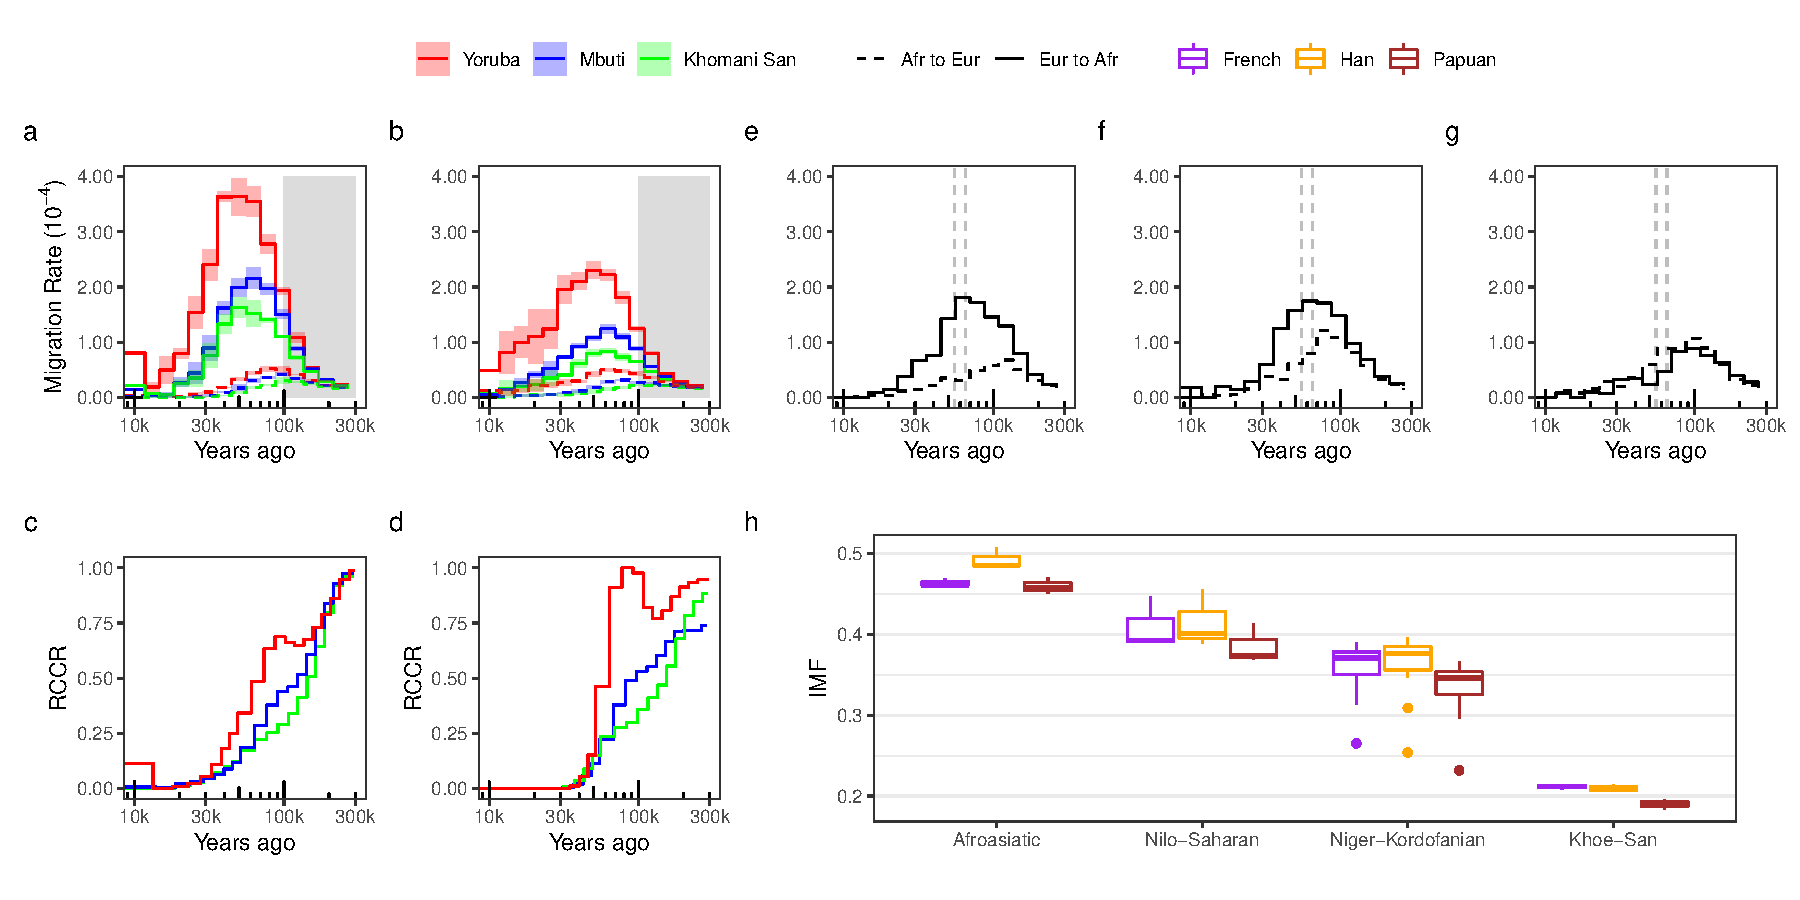
\includegraphics[width=\textwidth]{plot/new_mig_plot.pdf}
	\caption{ {\bf Migration rate inference} {\bf a}. Inferred migration between an African individual and a Han Chinese individual in the Simons Genome Diversity Panel (SGDP) estimated using {\tt SMCSMC}. Three replicates were performed, with the mean estimate plotted and standard deviation  shaded. Solid lines show inferred migration from Eurasians to Africans (forward in time) while dotted show the inverse. The {\tt SMCSMC} analysis used 10000 particles to estimate the posterior distribution of marginal trees, and 25 iterations of variational Bayesian inference to achieve converged parameter estimates. The shaded grey regions represents a time period where simulation shows {\tt SMCSMC} has very little power to infer migration (Supplemental Section \ref{simproc}).  {\bf b}. The same analysis as in a. except using individuals from the physically phased subset of the Human Genome Diversity Panel (HGDP), showing similar differences between populations but systematically lower migration overall. Three replications were performed to estimate error and the standard deviation is shaded. The same {\tt SMCSMC} settings were used as in a. {\bf c}. Relative cross-coalescence rate (RCCR) estimated by {\tt MSMC} in three different populations in the SGDP, supporting gene flow between Eurasians and Yorubans not shared by Mbuti or Khoe-San. 40 iterations were used to achieve parameter convergence. {\bf d}. The same analysis as in c. but performed on individuals in the physically phased subset of the HGDP, similarly supporting shared gene flow between the Yoruban and Eurasians not shared by Mbuti or Khoe-San. {\bf e}, {\bf f} and {\bf g}. Inferred migration rates from from data simulated under a two-island model with, from left to right, a backward Eurasia-to-Africa, a bidirectional, and a forward migration pulse lasting 10ky (dashed vertical lines) and replacing 40\% of the recipient population(s) approximately 60kya. The migration rate from Africa to Eurasia is not well estimated by {\tt SMCSMC} (see Figs.\ \ref{fig:backsim}--\ref{fig:fwdsim} and Supplemental Section \ref{simproc}), but SMCSMC is well powered to infer migration from Eurasia to Africa in this period. {\bf h}. Integrated total migration fraction (IMF) over the last 100 thousand years stratified by language phyla in the SGDP and comparison Eurasian population used to estimate migration. Afroasiatic (Mozabite, Saharawi, and Somali), Nilo-Saharan (Dinka, Luo, and Masai), Niger-Kordofanian (BantuHerero, BantuKenya, BantuTswana, Biaka, Esan, Gambian, Luhya, Mandenka, Mbuti, and Mende), and San (Khomani San and Ju hoan North) are grouped as in \cite{Fan2019}. Similar levels of migration are inferred from French and Han Chinese to all language groups, with significantly less migration from Papuan groups ($p\leq 0.05$, two-tailed paired t-test, Supplemental Table \ref{average_sgdp_migration_table}). }
	\label{migrationplot}
\end{figure}


\clearpage
\begin{figure}
    \centering
    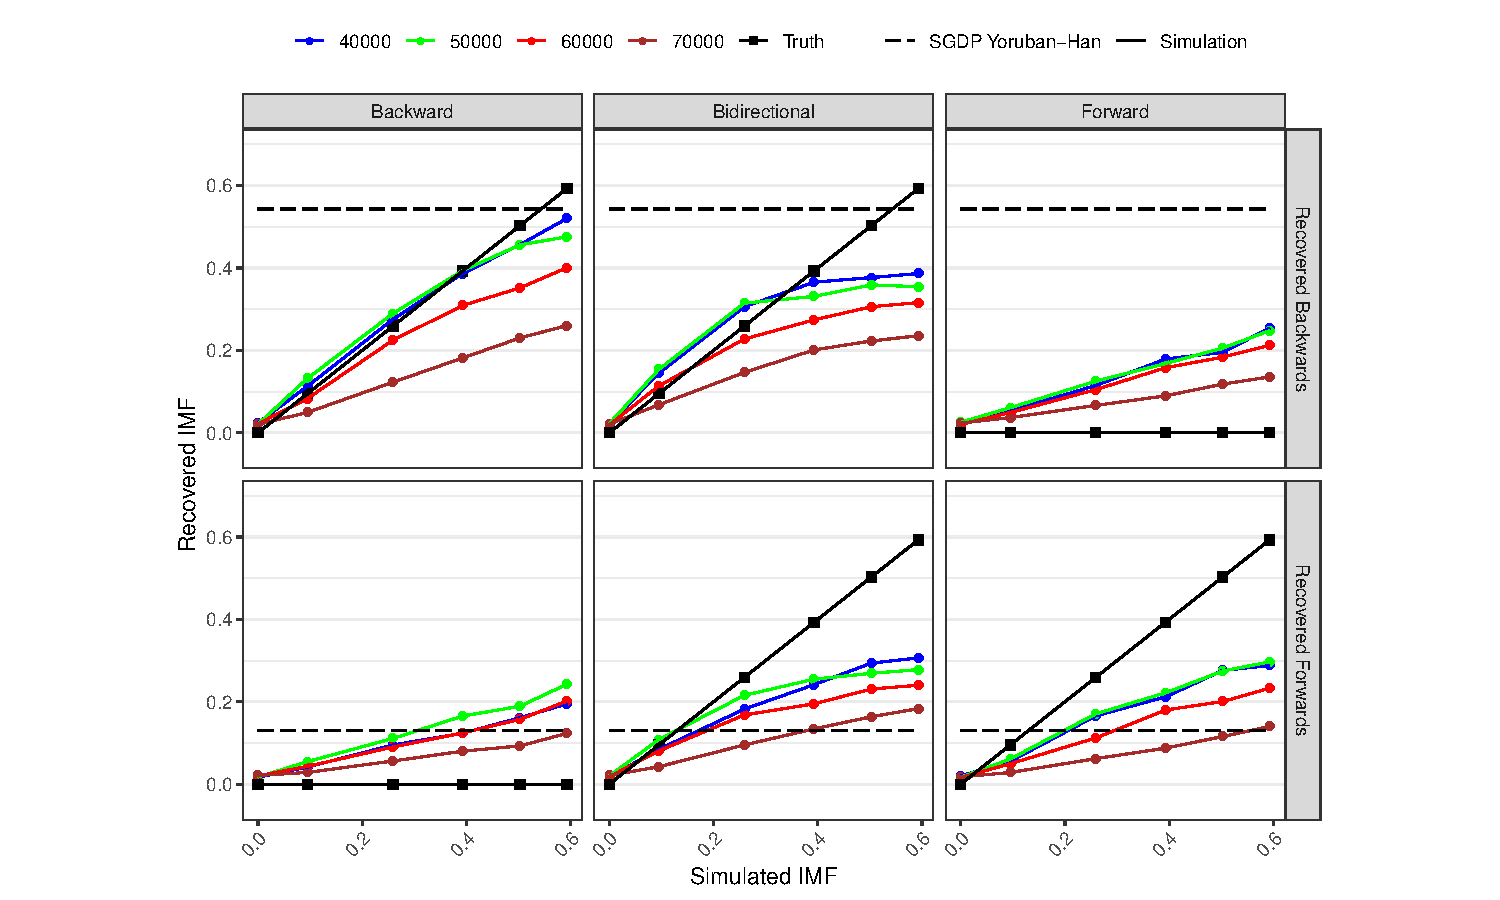
\includegraphics[width=\textwidth]{plot/sim_line_plot.pdf}
    \caption{\textbf{Simulation study}. {\tt SCRM} was used to simulate 1 Gigabase sequence data for two diploid individuals under three different migration models. Migration was simulated backwards (from a Eurasian-like population to an African-like population), forward (the inverse), and symmetrically (equal migration in both directions). The amount of migration indicates the proportion of the sink population replaced by the source over a 10000 year period which is simulated to occur 40, 50, 60, or 70kya. The total integrated migration fraction (IMF) recovered by {\tt SMCSMC} over the last 100ky is plotted and compared to the amount truly simulated. For reference, the IMF in either direction from 0-100kya for a Yoruban and Han individual is given in dashed lines.  5 iterations of variational Bayes and 5000 particles were used for inference. The effective population size model and additional details are given in Supplemental Section \ref{simproc}.}
    \label{fig:sim}
\end{figure}


\clearpage
\begin{figure}
	\centering
	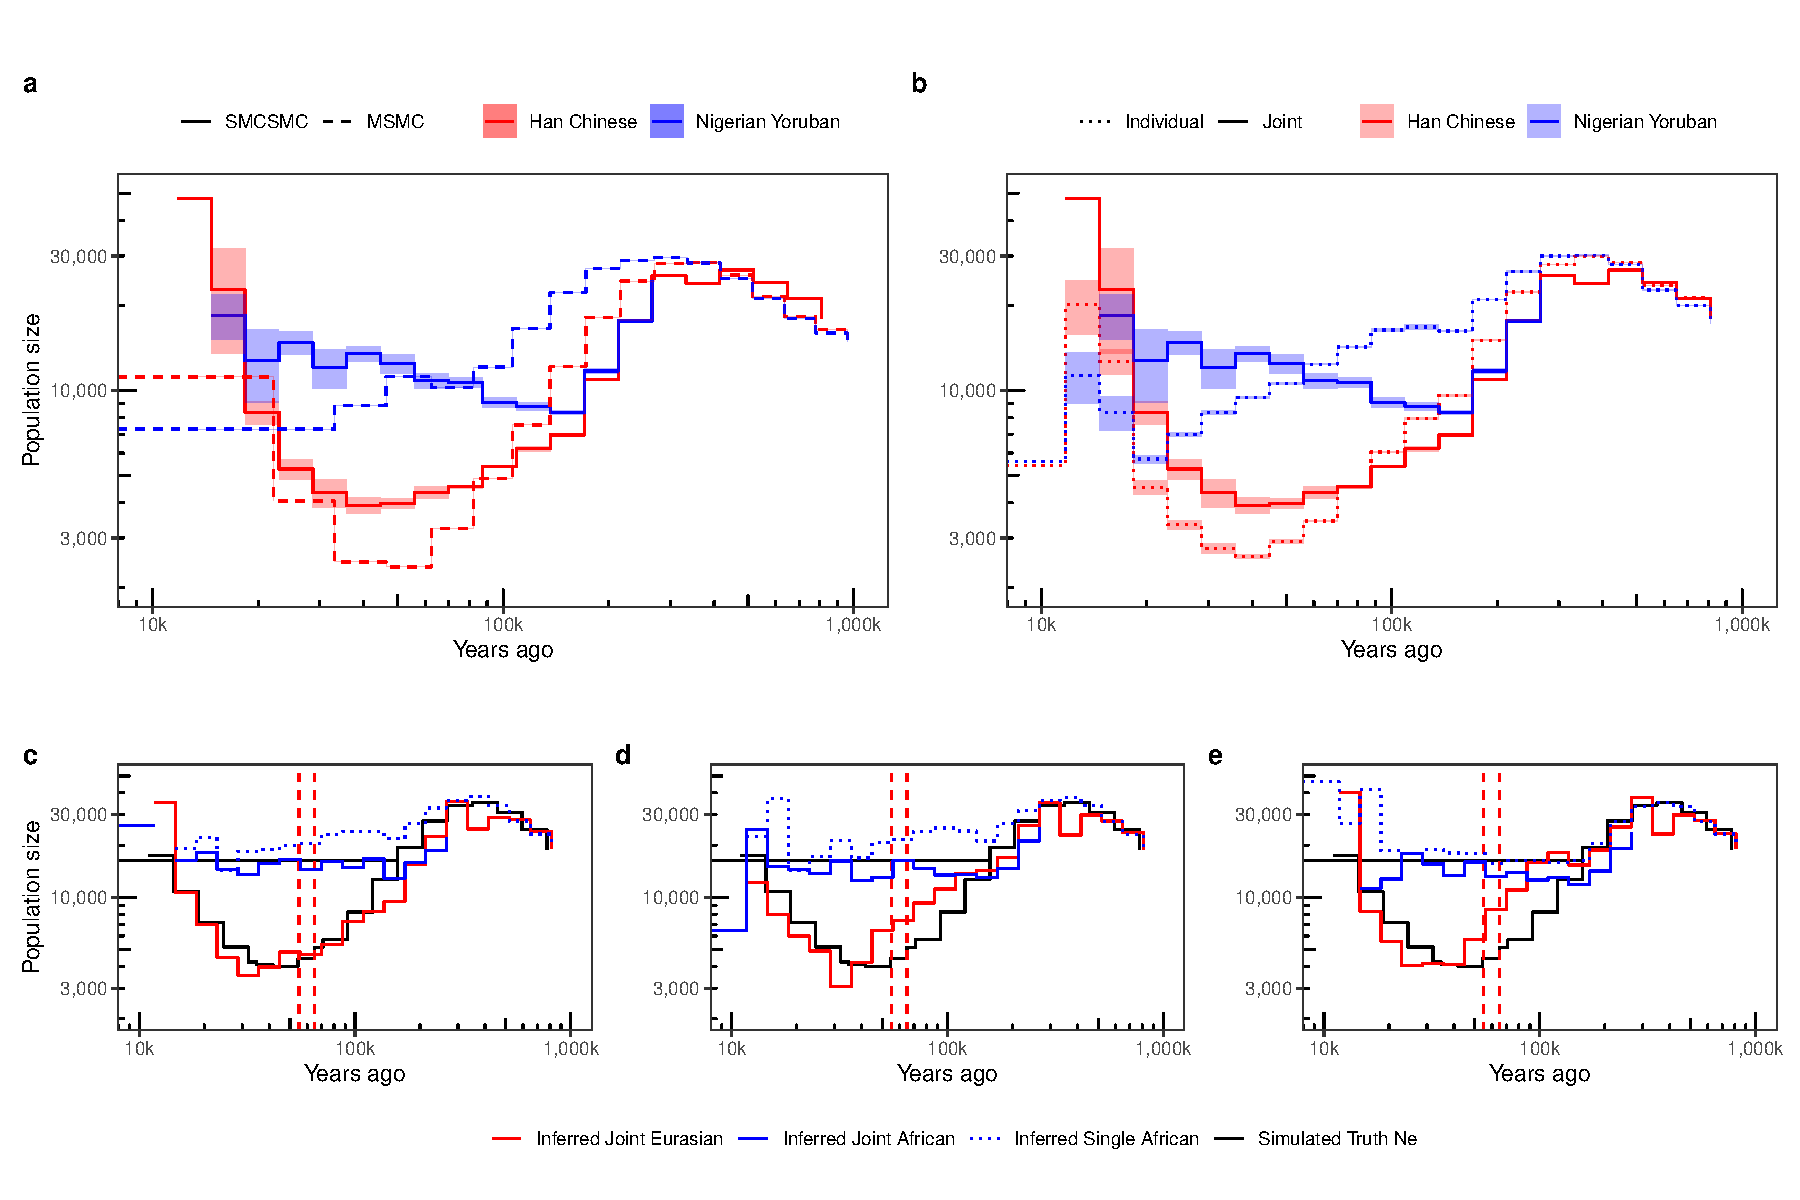
\includegraphics[width=\textwidth]{plot/new_ne_figure.pdf}
	\caption{{\bf Effective population size inference.} {\bf a.} Analyzing a Nigerian Yoruban and a Han Chinese individual from the Simons Genome Diversity Panel jointly in a two-island model with directional migration using {\tt SMCSMC} yields markedly lower $N_e$ estimates and a more recent apparent split time, than when the same data are analyzed using {\tt MSMC} with a model that does not explicitly include migration. Analyses for {\tt SMCSMC} repeated three times; range of the estimates shaded. {\bf b.} When each individual is analysed separately, using a model not including migration, $N_e$ estimates from {\tt SMCSMC} are similar to those of {\tt MSMC2}. (Joint estimate from {\bf a} included for comparison.) {\bf c, d,} and {\bf e.} 
	Inferred Eurasian and African $N_e$ from data simulated under a two-island model with, from left to right, a backward Eurasia-to-Africa, a bidirectional, and a forward  migration pulse lasting $10$ky (dashed vertical lines; same data as for Fig.\ \ref{migrationplot}{\bf e}-{\bf g}).  Particularly for the backward migration case, inferred $N_e$ under a two-island model tracks the true values (black) well, while inferred $N_e$ under a single-population model are inflated around the split time.
 All {\tt SMCSMC} analyses used 10000 particles and 25 variational Bayesian iterations; {\tt MSMC} analyses used 40 iterations (Supplemental Section \ref{simproc}).}
	%\caption{{ \bf Directional migration leads to bias in effective sample size estimates.} a. Joint inference of African ({\tt S\_Yoruba-1}) and Eurasian ({\tt S\_Han-1}) population sizes in both MSMC and SMCSMC. In green, SMCSMC inference is plotted for a single inference of the African genome without taking into account Eurasian migration. This analysis is performed for all three partner populations and all African populations in Supplemental Figure \ref{sgdp_ne}. For MSMC, 40 iterations were used to achieve convergence. For SMCSMC, 25 iterations and 10,000 particles were used. b. Inferred population size from three simulated migration scenarios. Black line denotes the true simulated demographic history. One gigabase of sequence was simulated using {\tt scrm} for backwards (migration from Eurasia to Africa), forwards (migration from Africa to Eurasia), and bidirectional migration. Green line denotes the inference on the African-like genome alone, without taking into account migration. A 40\% replacement was simulated between 55 and 65kya. Simulation results for a large number of situations are shown in Figures \ref{fig:backsim}, \ref{fig:fwdsim}, and \ref{fig:bisim} for the three directions respectively.}
	\label{neplot}
\end{figure}

%\clearpage
%\begin{figure}
%	\centering
%	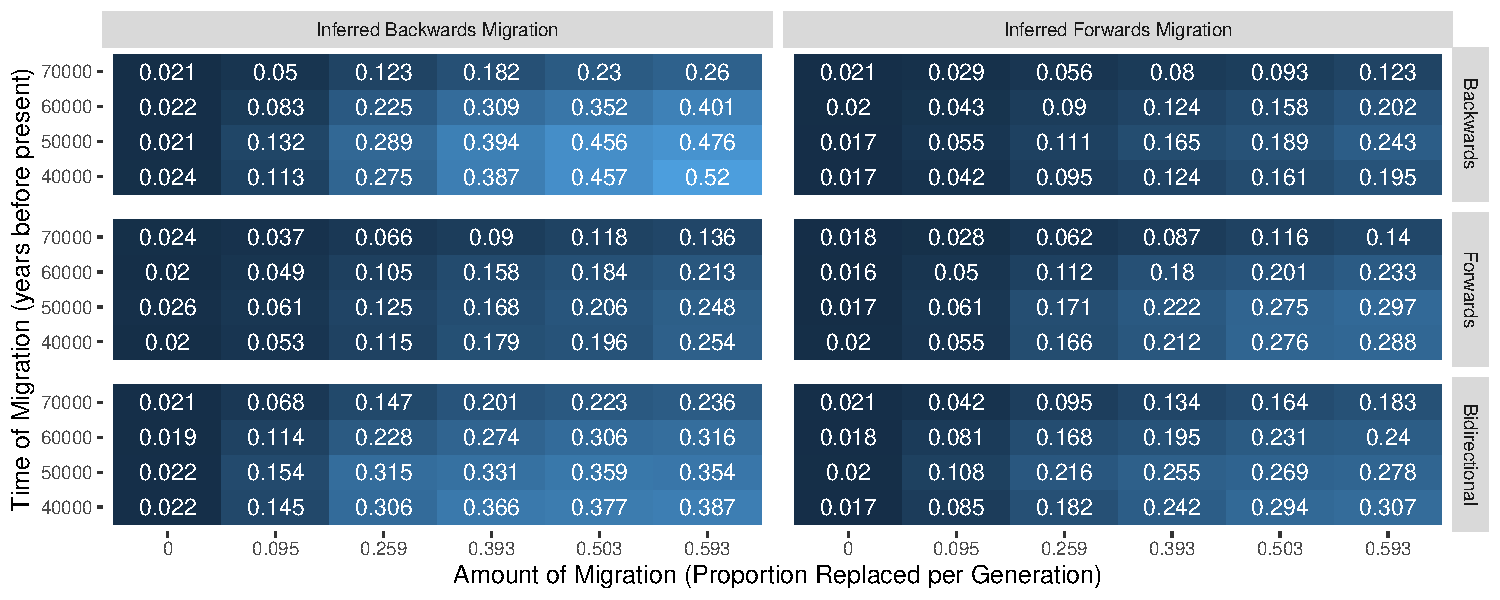
\includegraphics[width=\textwidth]{plot/recovered_migration_2.pdf}
%	\caption{ {\bf Simulation study concludes that {\tt SMCSMC} has power to detect a back-migration.} Under three different scenarios (migration ``backwards'' from Eurasia to Africa, migration ``forwards'' from Africa to Eurasia, and ``bidirectional'' migration, all forward in time), {\tt scrm} was used to simulate one gigabase of sequence and 5 iterations of {\tt SMCSMC} with 5000 particles were used to infer migration. The axis of each heatmap shows increasing simulated proportion replaced over 100,000 while the Y shows the midpoint of the migration simulated. The full migration and population size inference over time along with a more substantial set of simulations is available in Supplemental Section \ref{simproc}.}
%	\label{sim}
%\end{figure}

\begin{figure}
	\centering
	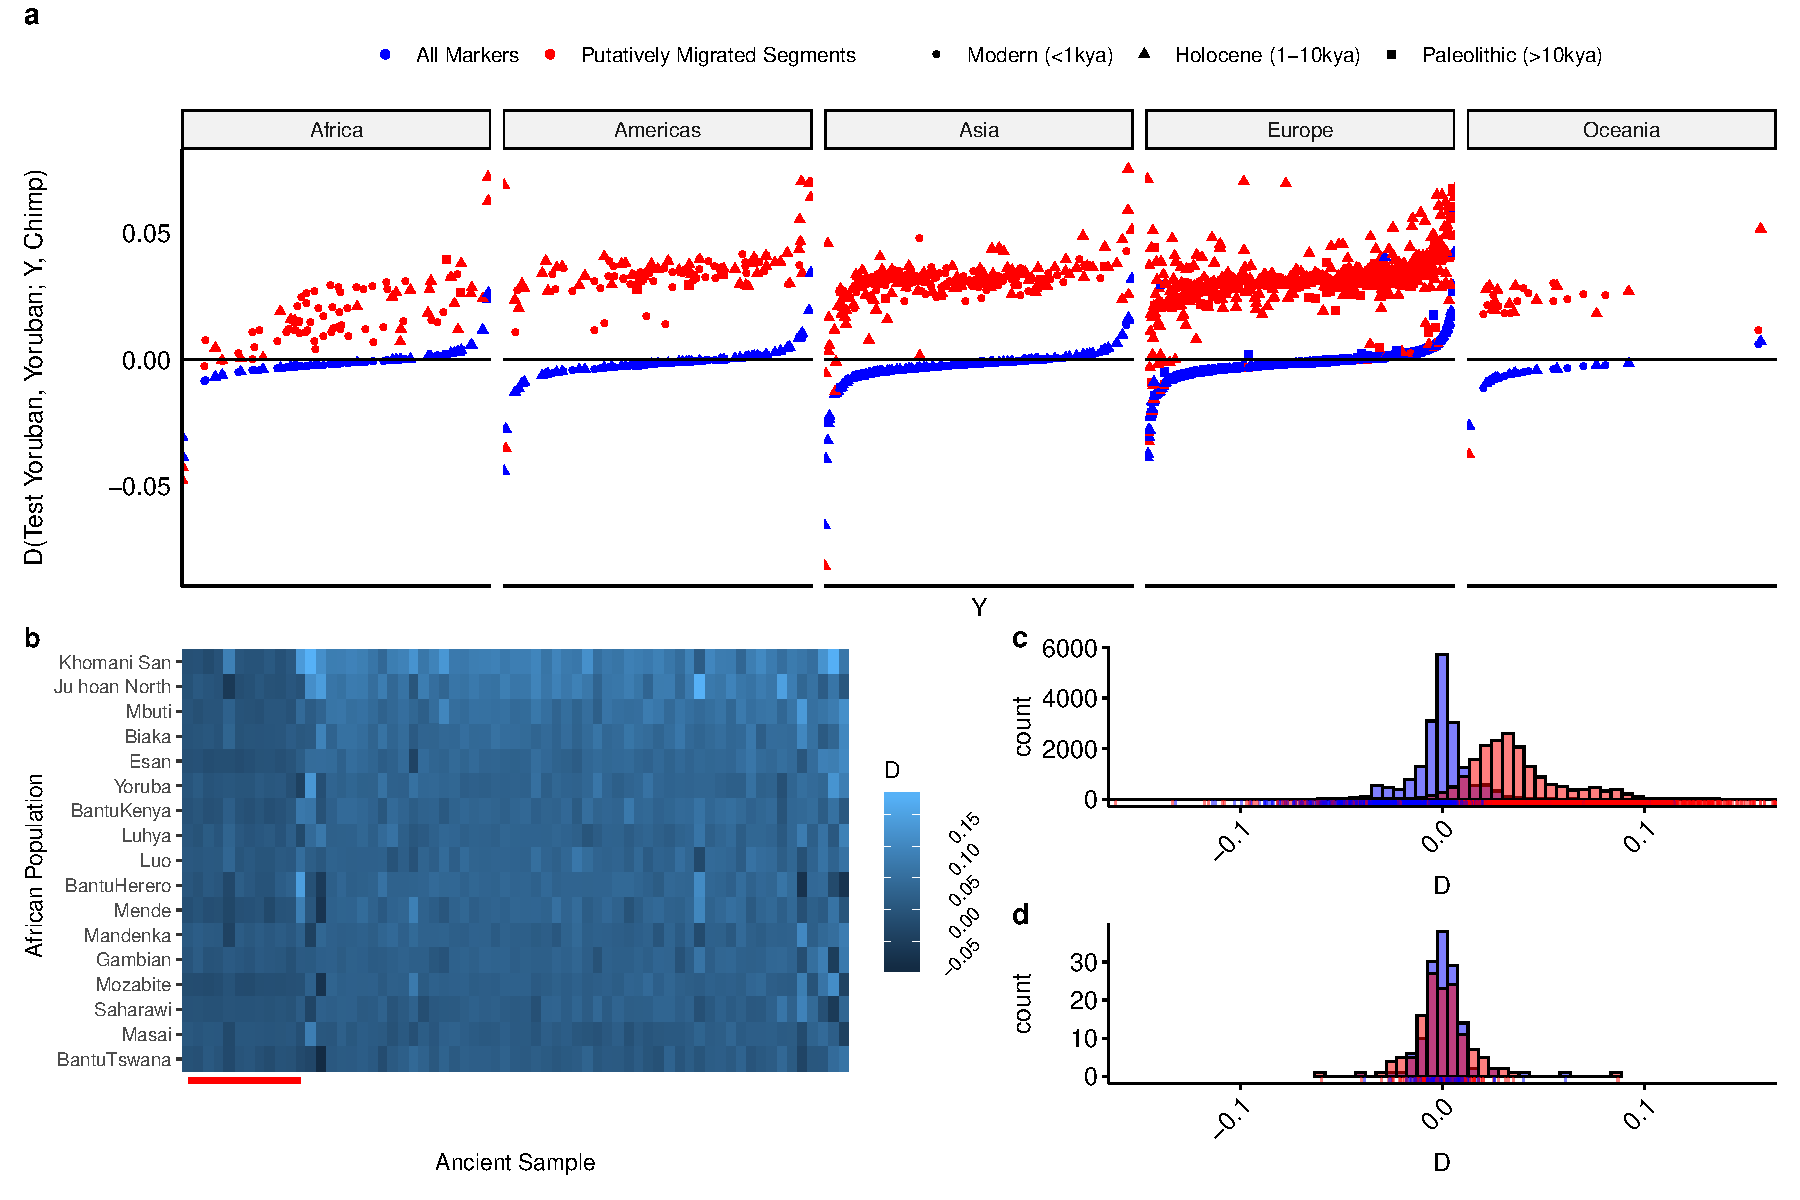
\includegraphics[width=\textwidth]{plot/new_dstats.pdf}
	\caption{{\bf African introgressed segments are more similar to Eurasians but show no Neanderthal or Denisovan enrichment.} {\bf a.} $D$(Test Yoruban, Comparison Yoruban; Test population, Chimpanzee) calculated for all populations in the Reich Human Origins dataset (see URLs). $D$ statistics in the putatively migrated segments are higher across the board in 3589 ancient, 6472 present day individuals. {\bf b.} The same $D$ statistic but computed for all African populations and individuals sampled from the Paleolithic. Neanderthal and Denisovan samples (marked with red bar) show low affinity to a Yoruban in putatively migrated segments. {\bf c.} Histogram of $D$ statistics computed in a. showing clear inflation of statistics calculated in segments (red) versus all markers (blue). {\bf d.} Subset of individuals from a. involving Neanderthal ($n = 6$),  Denisovan ($n=1$), and a unique mixture individual ($n=1$) with statistics calculated in segments (red) and all markers (blue) for all $n=17$ African individuals indicating no difference in this population.} 
	\label{dstats}
\end{figure}

\begin{figure}
    \centering
    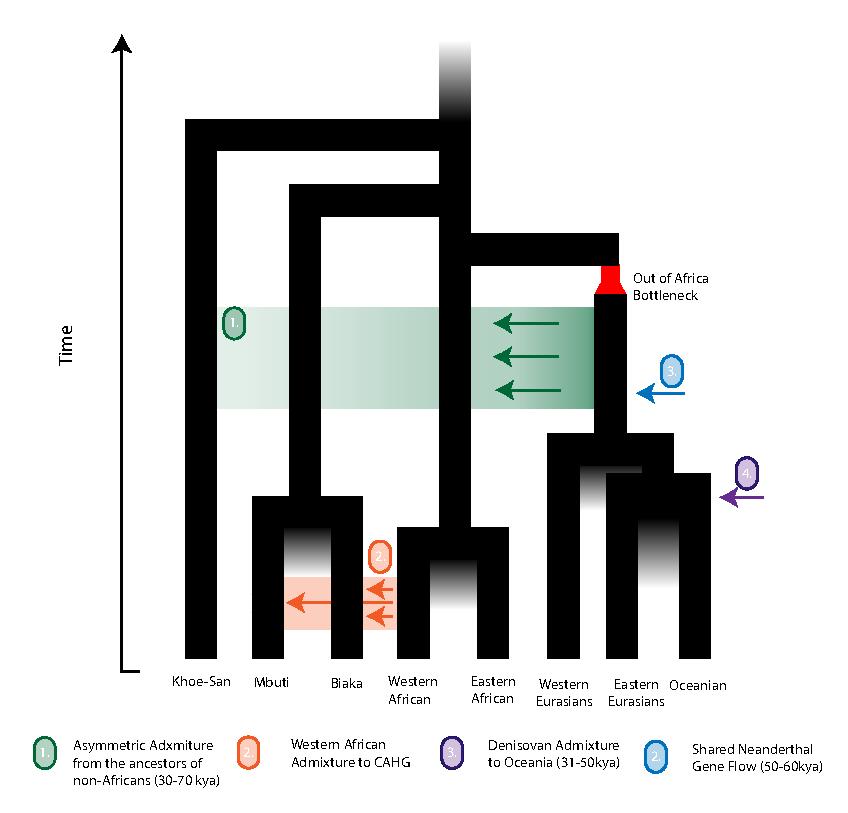
\includegraphics[width=0.9\textwidth]{plot/simple_demography_v5.pdf}
    \caption{ {\bf Proposed model for the diversification of modern human lineages.}
    The proposed admixture from ancestors of present-day non-Africans is indicated in green.
    Several elements of this model remain unresolved, including the timing of the proposed admixture into Central and Southern Hunter Gatherer populations and these population's branching order, gene flow from an unsampled archaic African human lineage, and the different episodes of Neanderthal and Denisovan admixture. Date ranges for the diversification of Central and Southern African Hunter Gatherers \cite{Mallick2016}, Out of Africa migration \cite{Lipson2019}, Eastern / Western Eurasian diversification \cite{Schiffels2014a}, Eastern / Western African diversification \cite{Fan2019}, Oceanian / Eastern Eurasian diversification \cite{Lipson2017}, the split of the Mbuti from Biaka \cite{Mallick2016}, Neanderthal gene flow \cite{Sankararaman2012}, and Denisovan Gene flow \cite{Malaspinas2016} may be found in references given. }
    \label{fig:simple_dem}
\end{figure}

\newpage
\clearpage
\emergencystretch=1em
\printbibliography
\newpage

%%
%% supplementary section
%%

\begin{center}
\Large Supplementary Material
\end{center}

\setcounter{section}{0}
\renewcommand{\thesection}{S\arabic{section}}%
\setcounter{table}{0}
\renewcommand{\thetable}{S\arabic{table}}%
\setcounter{figure}{0}
\renewcommand{\thefigure}{S\arabic{figure}}%

\addtocontents{toc}{\protect\setcounter{tocdepth}{2}}

\vskip3\baselineskip
\tableofcontents
\newpage

\section{Supplemental Figures}


%S1
\begin{figure}
    \centering
    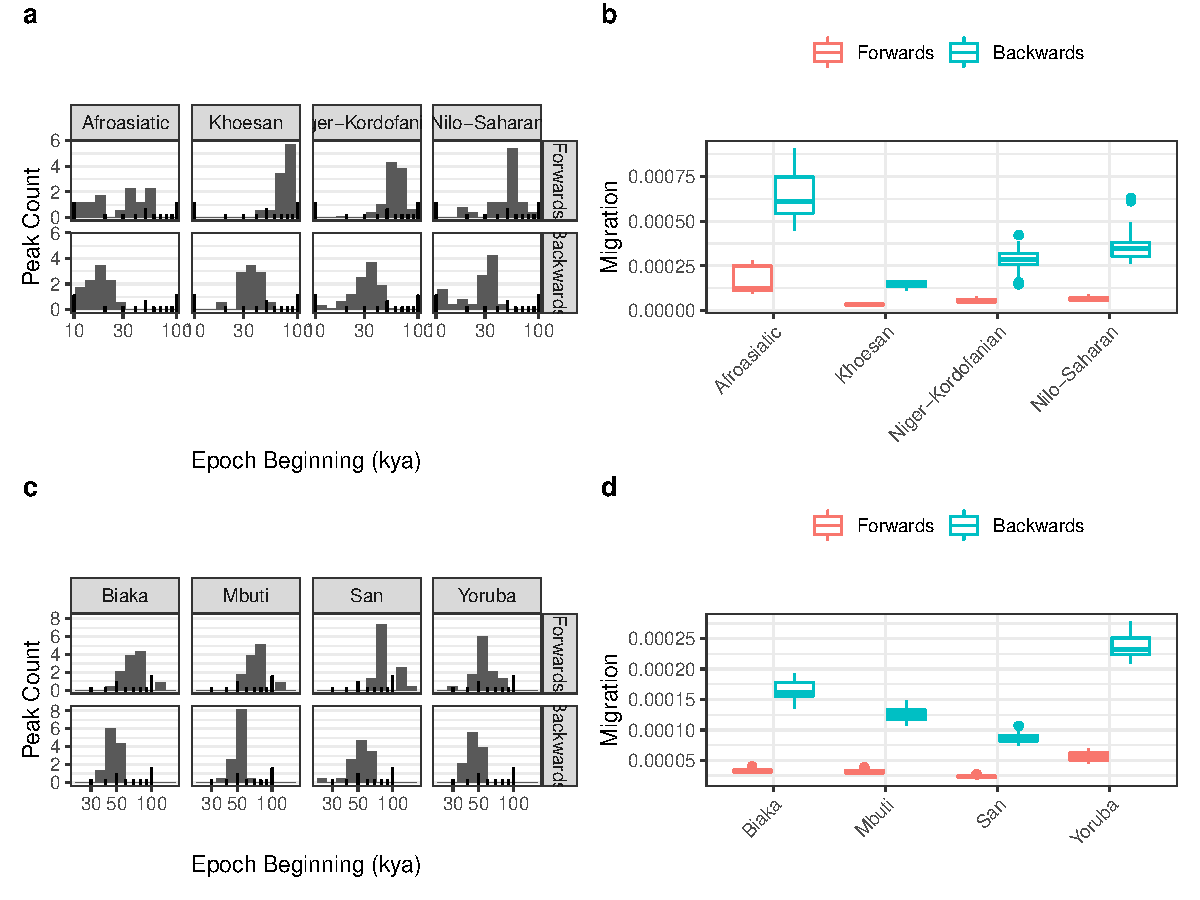
\includegraphics[width=\textwidth]{plot/peaks.pdf}
    \caption{{\bf Timing and average maximum rate of directional migration in HGDP and SGDP.} {\bf a} Migration is inferred in evenly spaced epochs on the log scale from 3.8 thousand to 3.8 million years ago. For each population in the SGDP, we record the epoch with the highest inferred directional migration rate (the ``peak'' of migration) and plot this as a histogram. Backwards migration refers to migration from Eurasians to Africans, whilst forward represents the inverse. {\bf b} In the epochs of highest migration identified in a., we record the inferred rate per population and plot these as a boxplot. Whiskers represent 1.5 times the interquartile range. The migration rate is given in proportion of the population replaced per generation. {\bf c} and {\bf d} represent the same analyses as in a. and b. calculated for the Human Genome Diversity Panel, rather than the SGDP.}
    \label{fig:peaks}
\end{figure}
\newpage

%S2
\begin{figure}
	\centering
	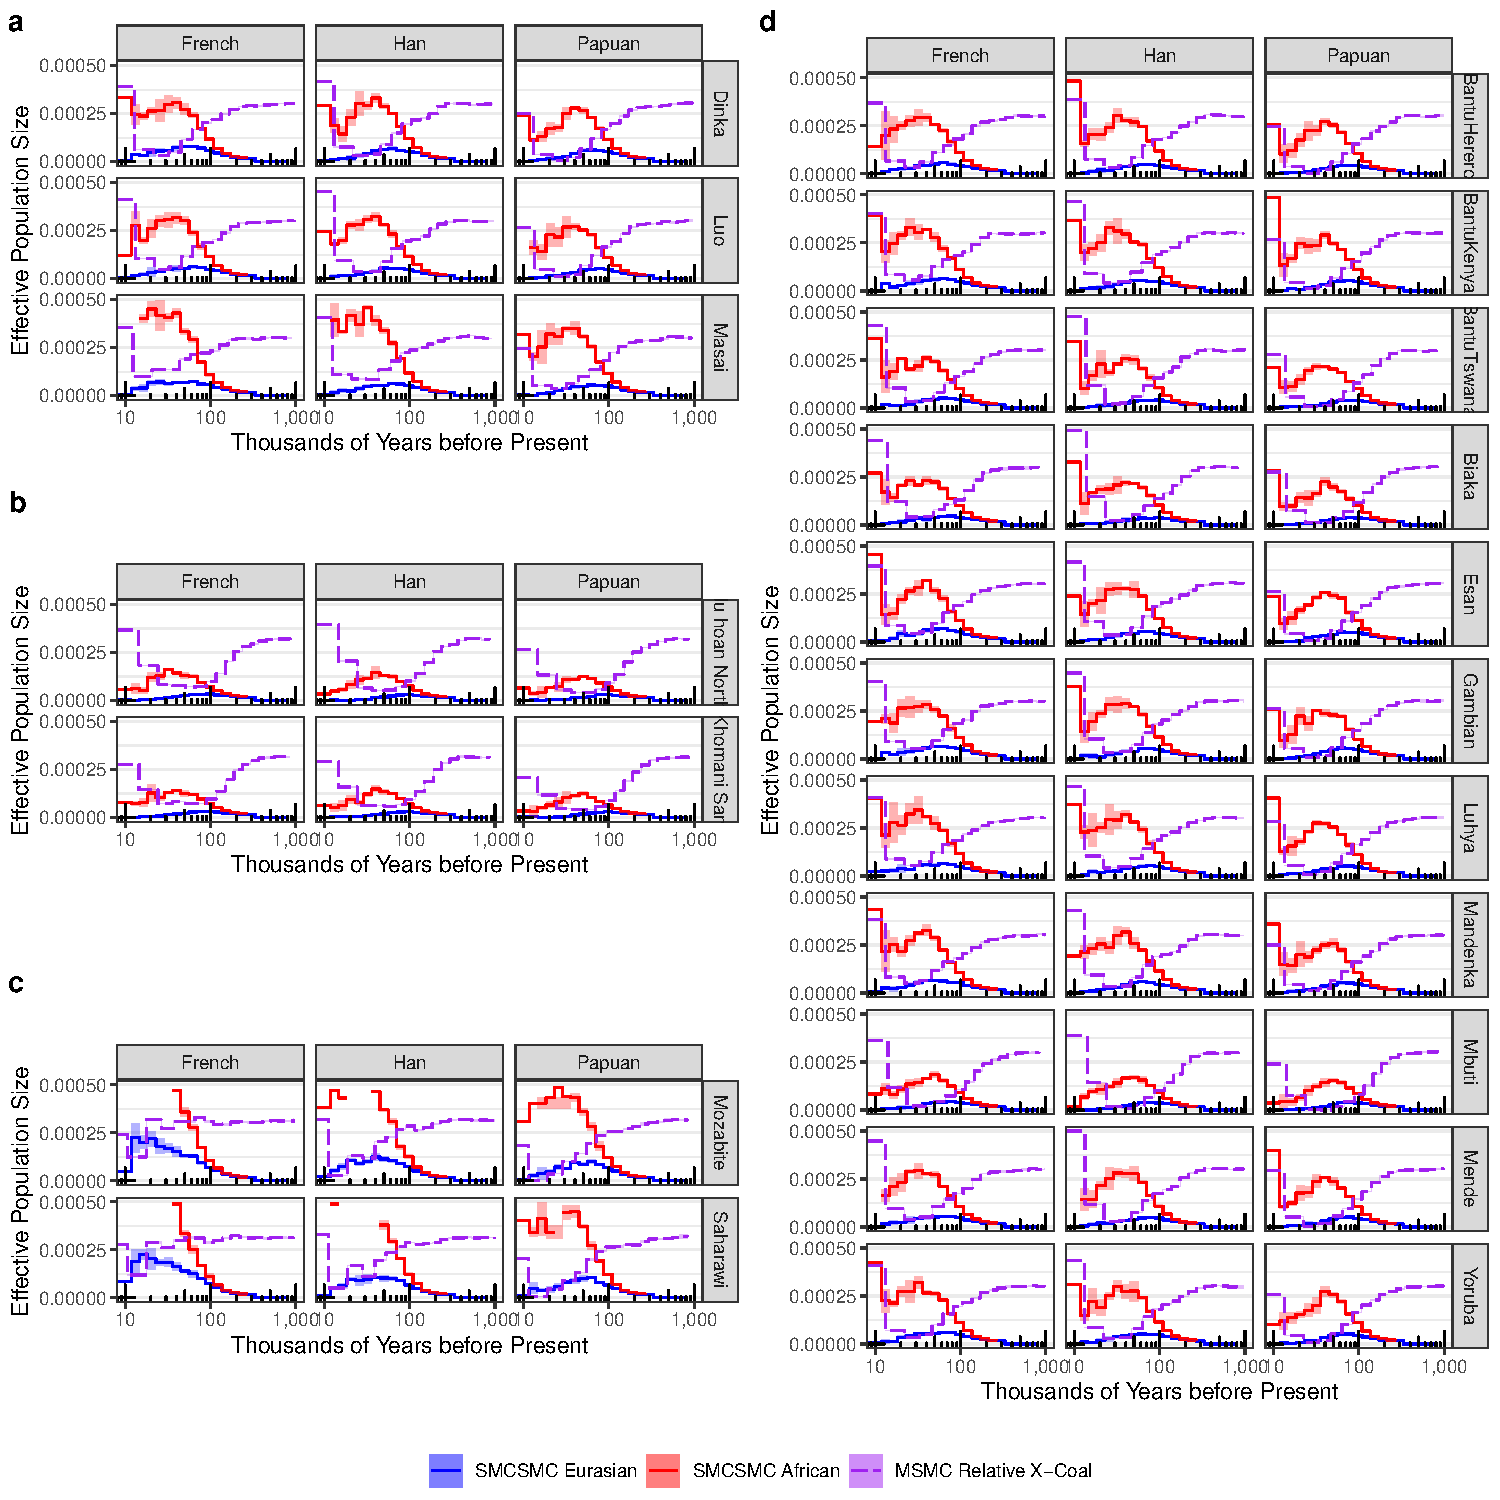
\includegraphics[width=0.95\linewidth]{plot/sgdp_mig_new.pdf}
	\caption{{\bf Inference of directional migration in the Simons Genome Diversity Project.} The {\tt SMCSMC} particle filter was used to infer directional migration rates in both directions from one of three Eurasian populations (French, Han, and Papuan) to one of 18 African populations. 5000 particles were used to approximate the ancestral recombination graph with 10 iterations of variational Bayesian inference to update demographic parameter values. Panels represent a. Nilo-Saharan, b. KhoeSan, c. Afroasiatic, and d. Niger-Kordofanian language families. Alongside the {\tt SMCSMC} inference, we use {\tt MSMC2} to infer the relative cross coalescent rate (RCCR) with default settings and 20 iterations for convergence.}	
	\label{sgdp_mig}
\end{figure}
\newpage

%S3






%S11
\begin{figure}
    \centering
    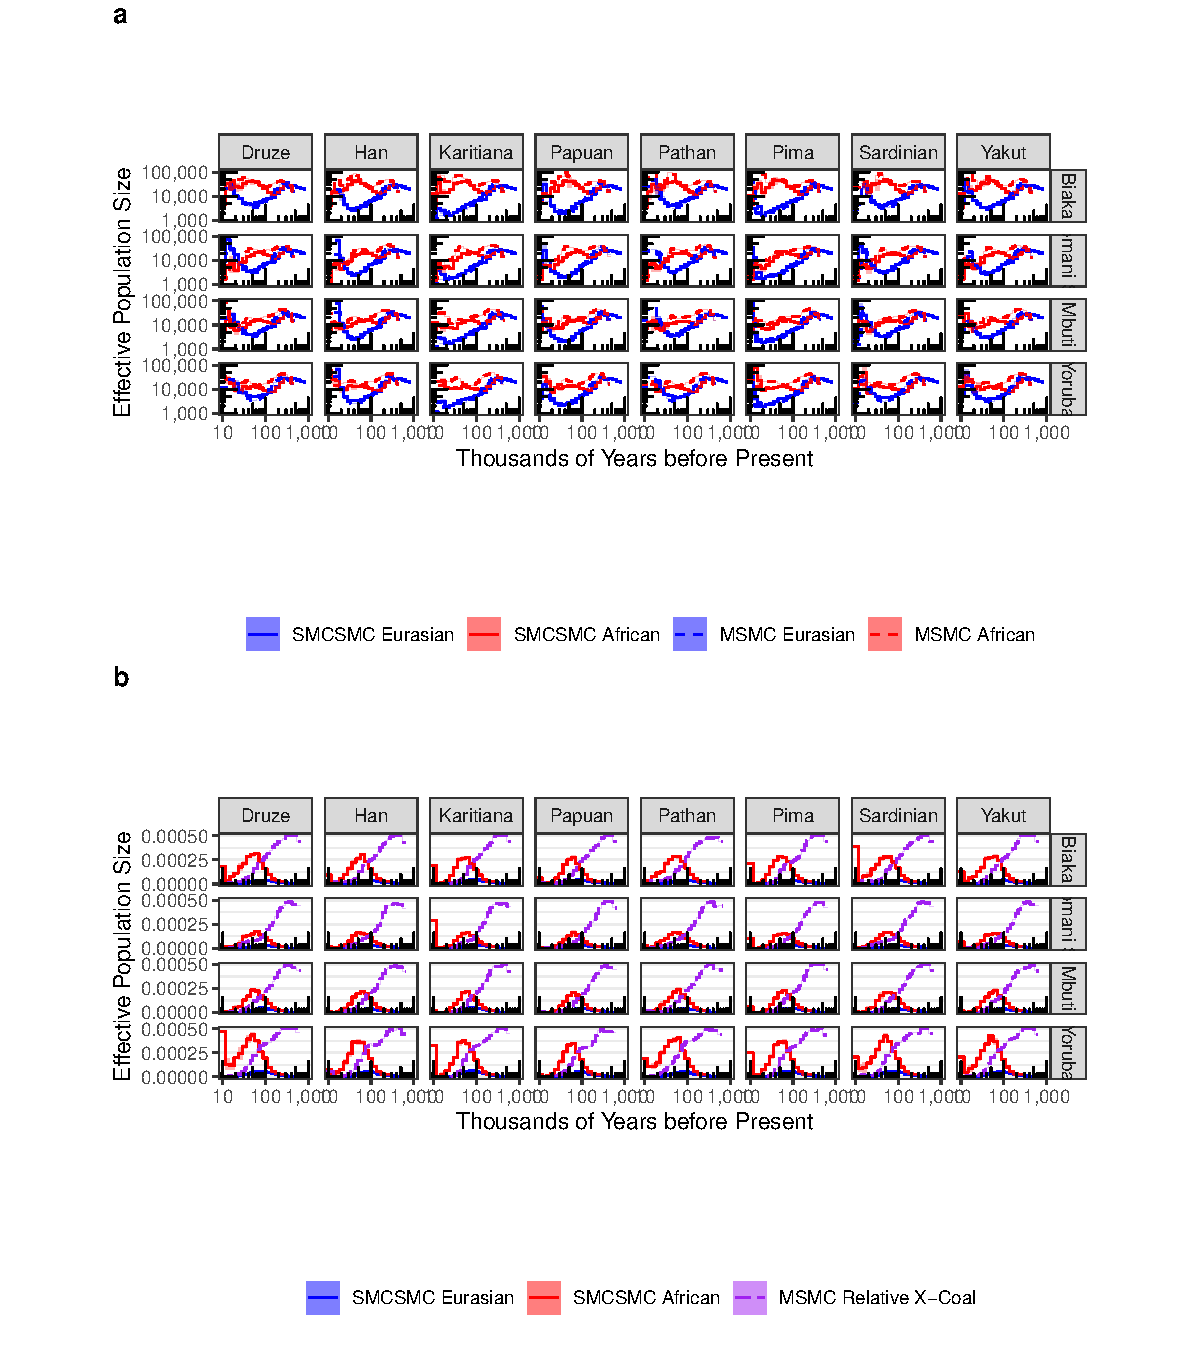
\includegraphics[width=0.9\textwidth]{plot/subset_ne_mig.pdf}
    \caption{ {\bf Demographic inference in a matched subset of the Simons Genome Diversity Panel}. {\bf a.} {\tt SMCSMC} and {\tt MSMC2} inferred effective population size of several populations in the Simons Genome Diversity Panel. These samples were selected to match, as closely as possible, those in the physically phased subet of the Human Genome Diversity Project panel. {b.} Inferred migration using {\tt SMCSMC} in the Simons Genome Diversity Panel along with the scaled relative cross-coalescent rate estimated by {\tt MSMC2}.  10,000 particles were used to approximate the ancestral recombination graph in the {\tt SMCSMC} particle filter and 25 iterations were used to update demographic parmaeters. 20 iterations were used for {\tt MSMC2}.}
    \label{fig:hgdp_sgdp}
\end{figure}


%S7
\begin{figure}
	\centering
	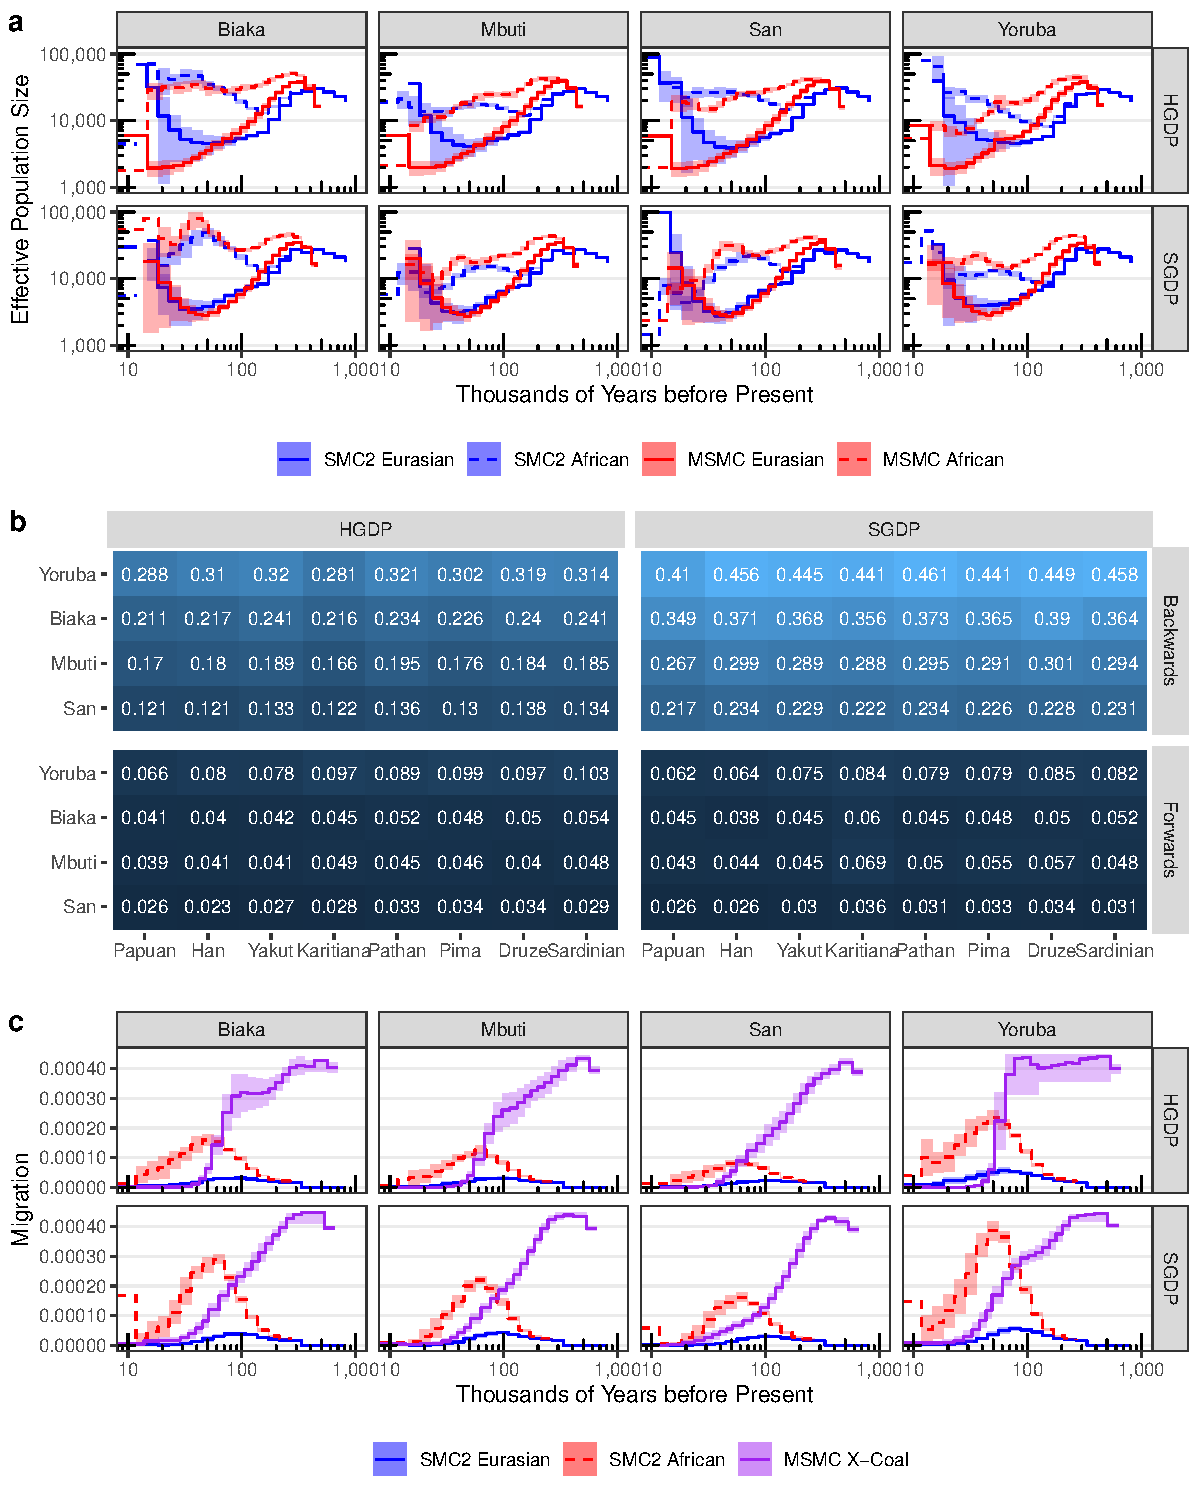
\includegraphics[width=0.7\textwidth]{plot/both_figure.pdf}
	\caption{{\bf Inference of directional migration is comparable between data sets and phasing strategies.} We used {\tt SMCSMC} as in \ref{data-analysis} to simultaneously infer directional migration rates and effective population size in the 36 genome physically phased subset of the Human Genome Diversity Panel. We match these 36 genomes with comparable individuals in the Simons Genome Diversity Panel (with the exception of one Papuan population, which has no comparable population in the SGDP) and perform an identical analysis. {\bf a.} Average $N_e$ estimate across four populations in the physically phased subset of the HGDP and the subset of SGDP used to compare with HGDP inference. Inference of population size is averaged over eight Eurasian populations, with the bars representing standard deviation. For {\tt MSMC2}, the time indexes were averaged to have consistent start and stop times for the steps. {\bf b.} Inferred integrated migration fraction (IMF) from Africa to Eurasians (forwards) and from Eursaians to Africans (backwards) between 40 and 70 kya (see Methods). {\bf c.} Directional migration inference in African populations averaged over Eurasian partners in the two data sets. Shaded regions denote standard deviations. For {\tt MSMC}, the time indexes were averaged to have consistent start and stop times for plotting.}
	\label{fig:both}
\end{figure}


%s4
%\begin{figure}
%    \centering
%    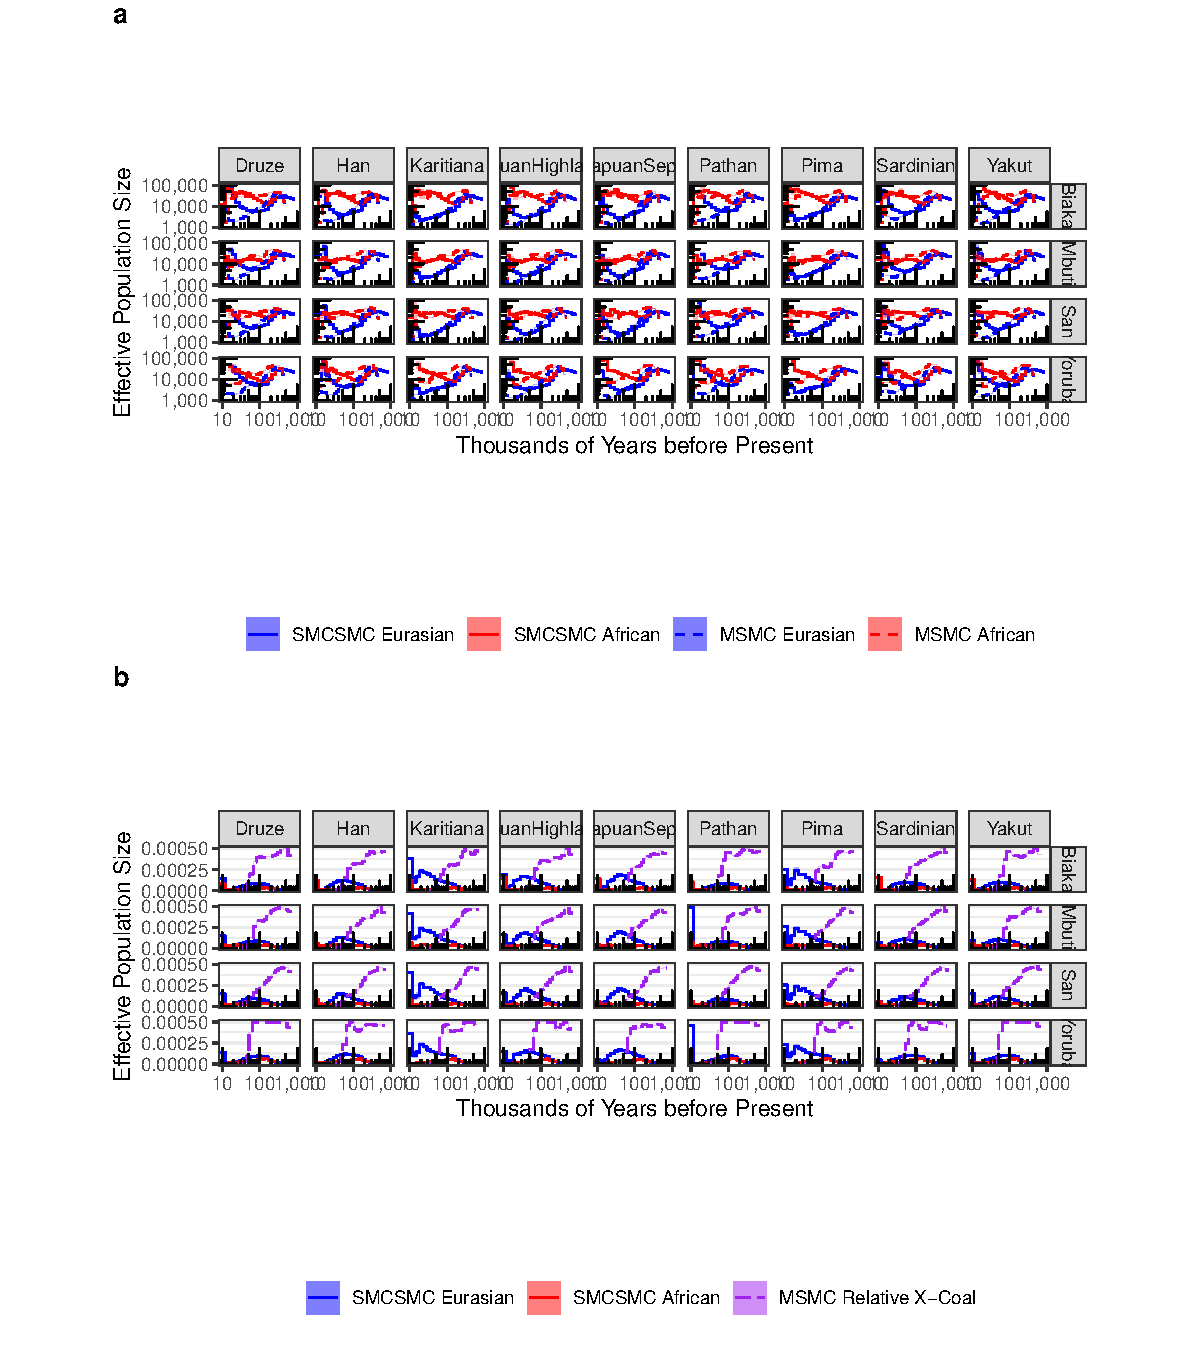
\includegraphics[width = \textwidth]{plot/hgdp_ne_mig.pdf}
%    \caption{Demographic inference in a subset of the Human Genome Diversity Panel. a.Historical inferred effective population size in the physically phased subset of the Human Genome Diversity Panel using {\tt SMCSMC} and {\tt MSMC}. 10000 particles and 25 iterations were used to achieve convergence for the former, while 40 iterations were used with the latter. b) Historical inferred directional migration in the physically phased subset of the Human Genome Diversity Panel using {\tt SMCSMC}.}
%    \label{fig:hgdp}
%\end{figure}


%S5
\begin{figure}[p!]
	\centering
	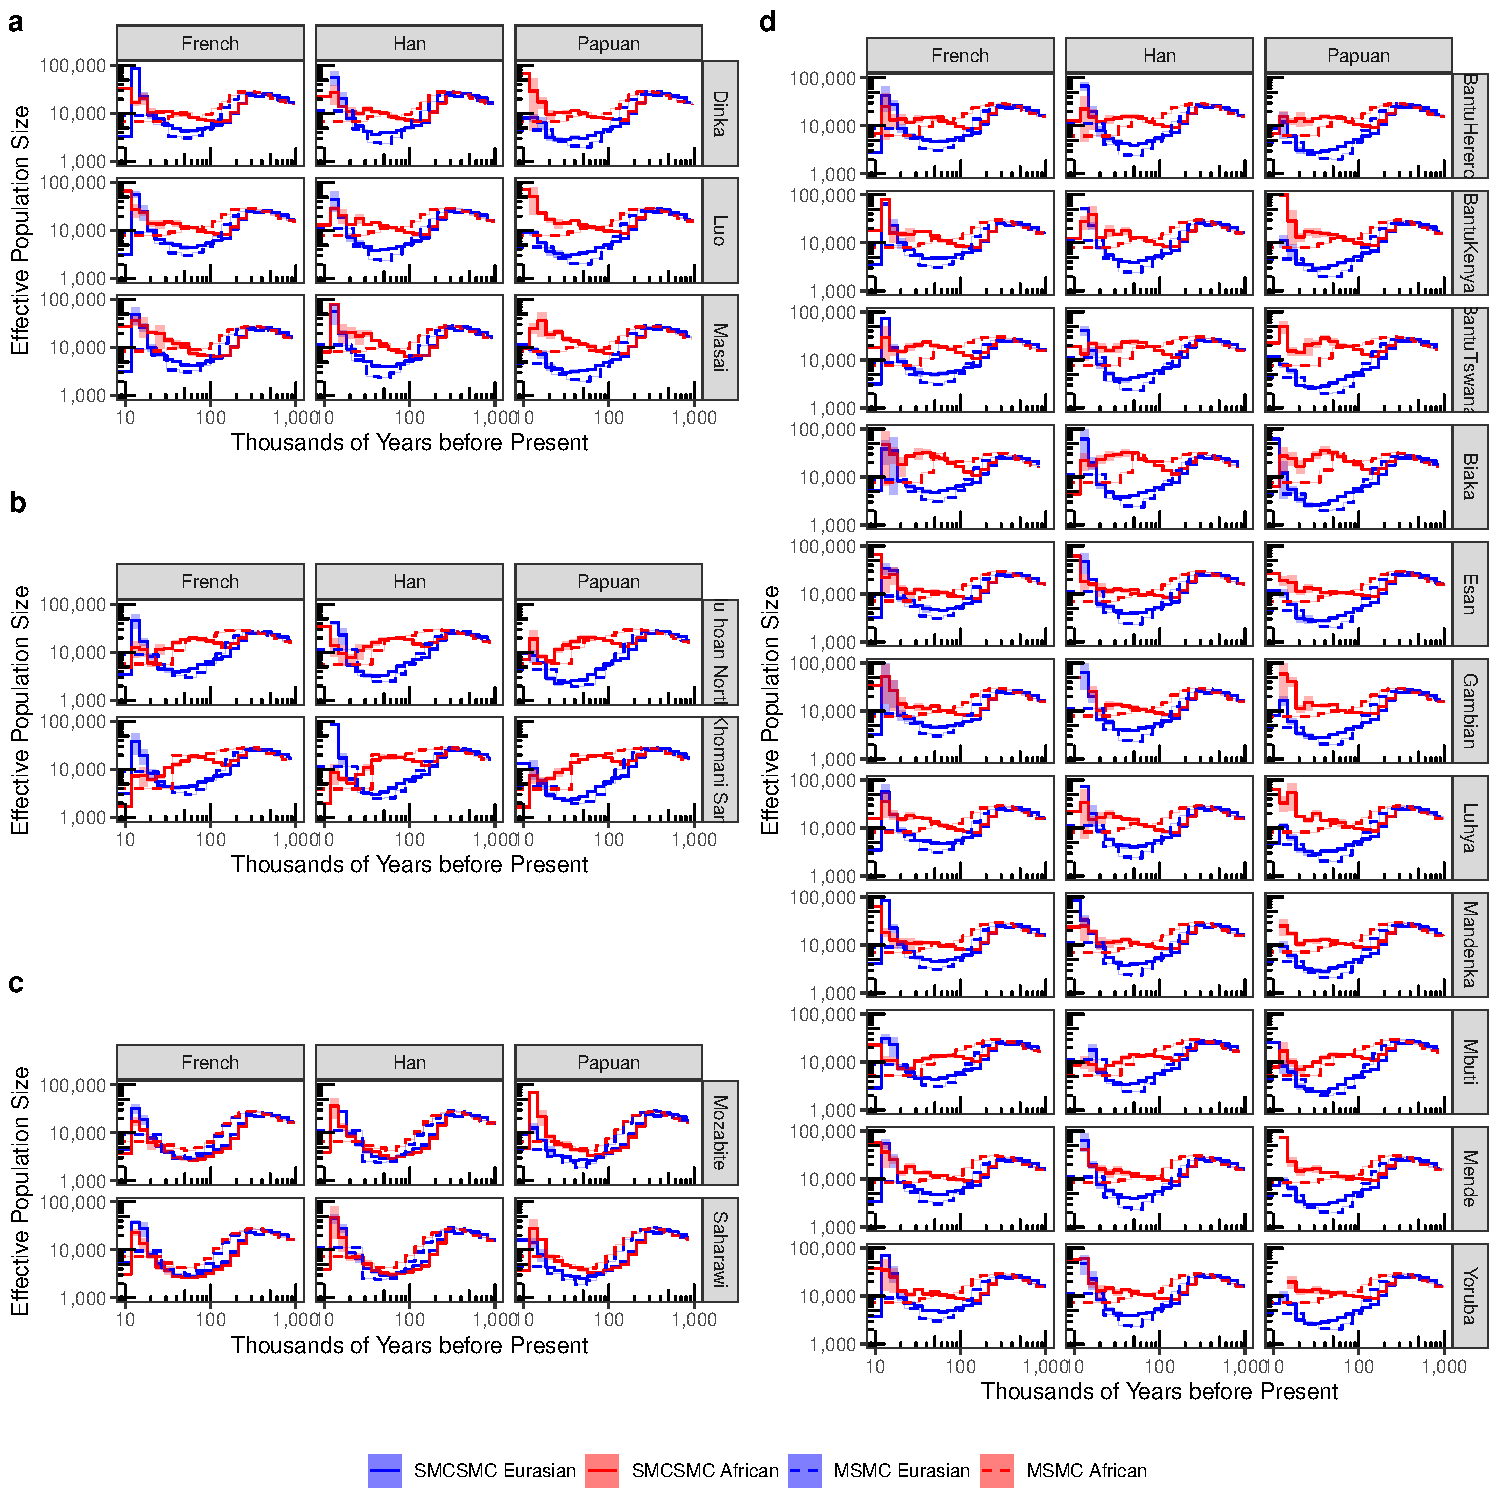
\includegraphics[width=0.95\linewidth]{plot/sgdp_ne_new.pdf}
	\caption{{\bf Inference of historical effective population size in the Simons Genome Diversity Project.} The {\tt SMCSMC} particle filter was used to infer directional migration rates and effective population size in both directions from one of three Eurasian populations (French, Han, and Papuan) to one of 18 African populations. 5000 particles were used to approximate the ancestral recombination graph with 10 iterations of variational Bayesian inference to update demographic parameter values. Panels represent a. Nilo-Saharan, b. KhoeSan, c. Afroasiatic, and d. Niger-Kordofanian language families. Alongside the {\tt SMCSMC} inference, we use {\tt MSMC2} to infer the same values with default settings and 20 iterations for convergence.}	
	\label{sgdp_ne}
\end{figure}
\newpage







\begin{figure}
	\centering
	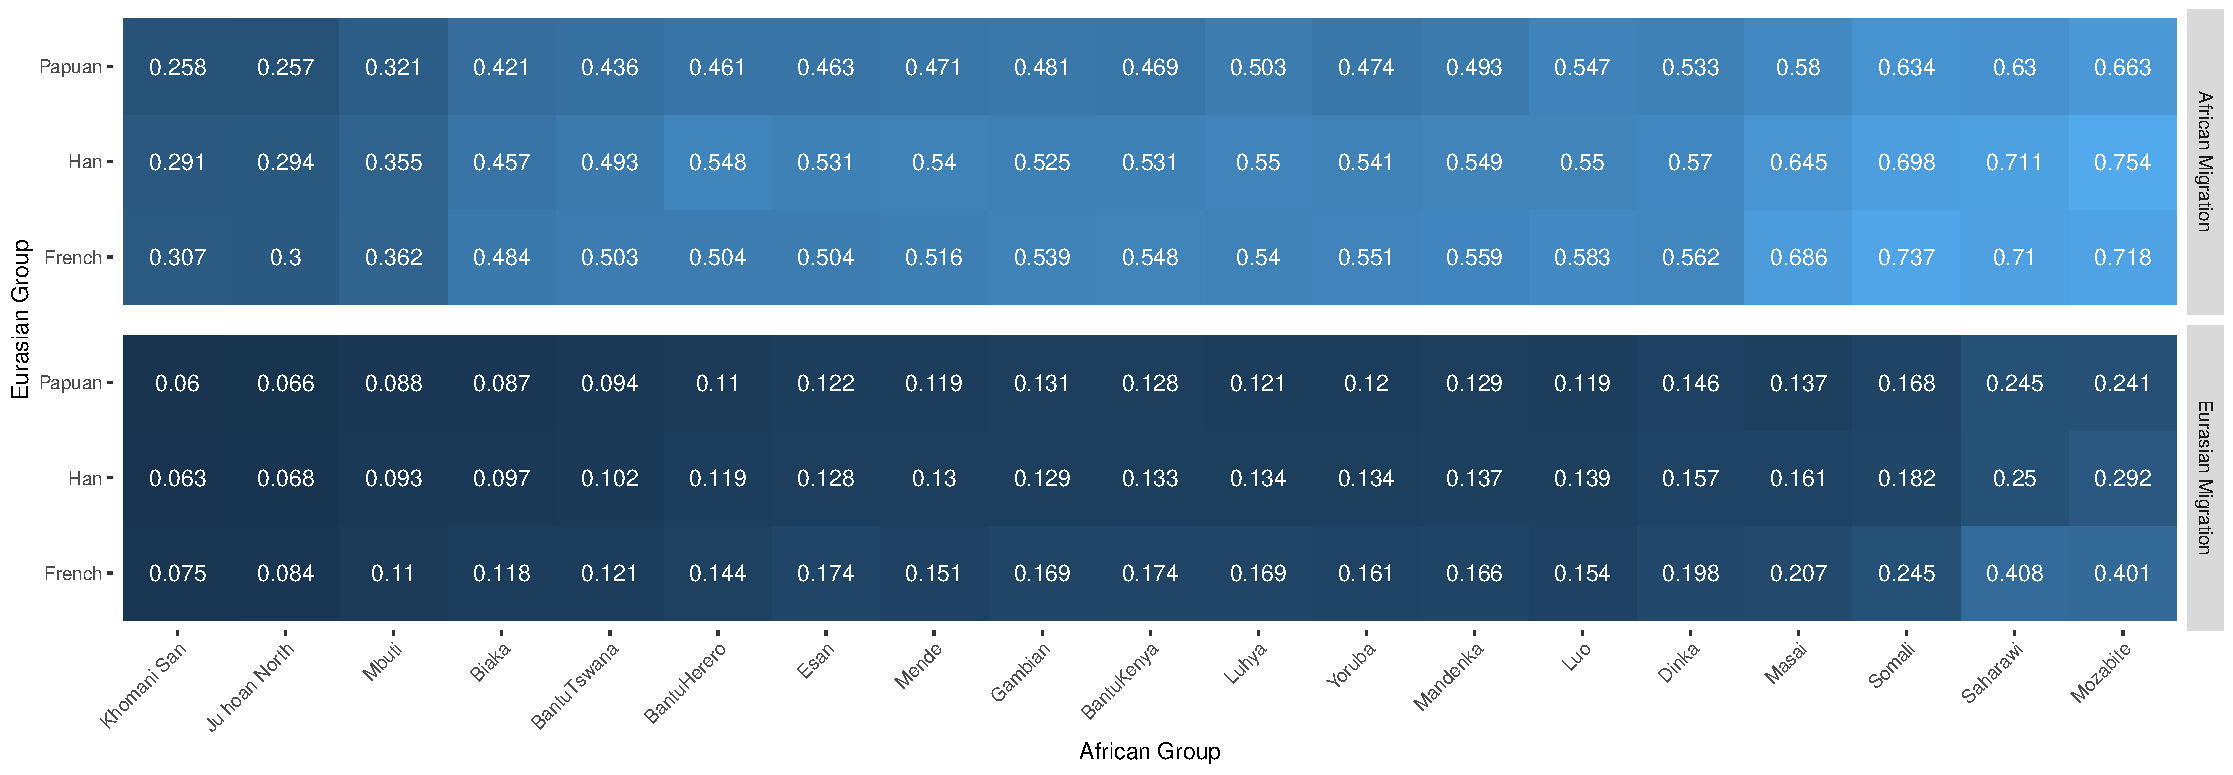
\includegraphics[width=\textwidth]{plot/integrated_sgdp.pdf}
	\caption{{\bf Integrated migration fraction 40--70kya in {\tt SMCSMC} analysed SGDP populations.} Following the analysis in Supplemental Section \ref{data-analysis}, directional migration was integrated by finding the cumulative probability of an individual migrating during the specified epoch. Directional migration backwards from Eurasia to Africa and forwards from Africa to Eurasia (both forward in time) are reported separately. Displayed is the average values from three technical replicates.}
	\label{sgdp_heatmap}
\end{figure}

\begin{figure}
    \centering
    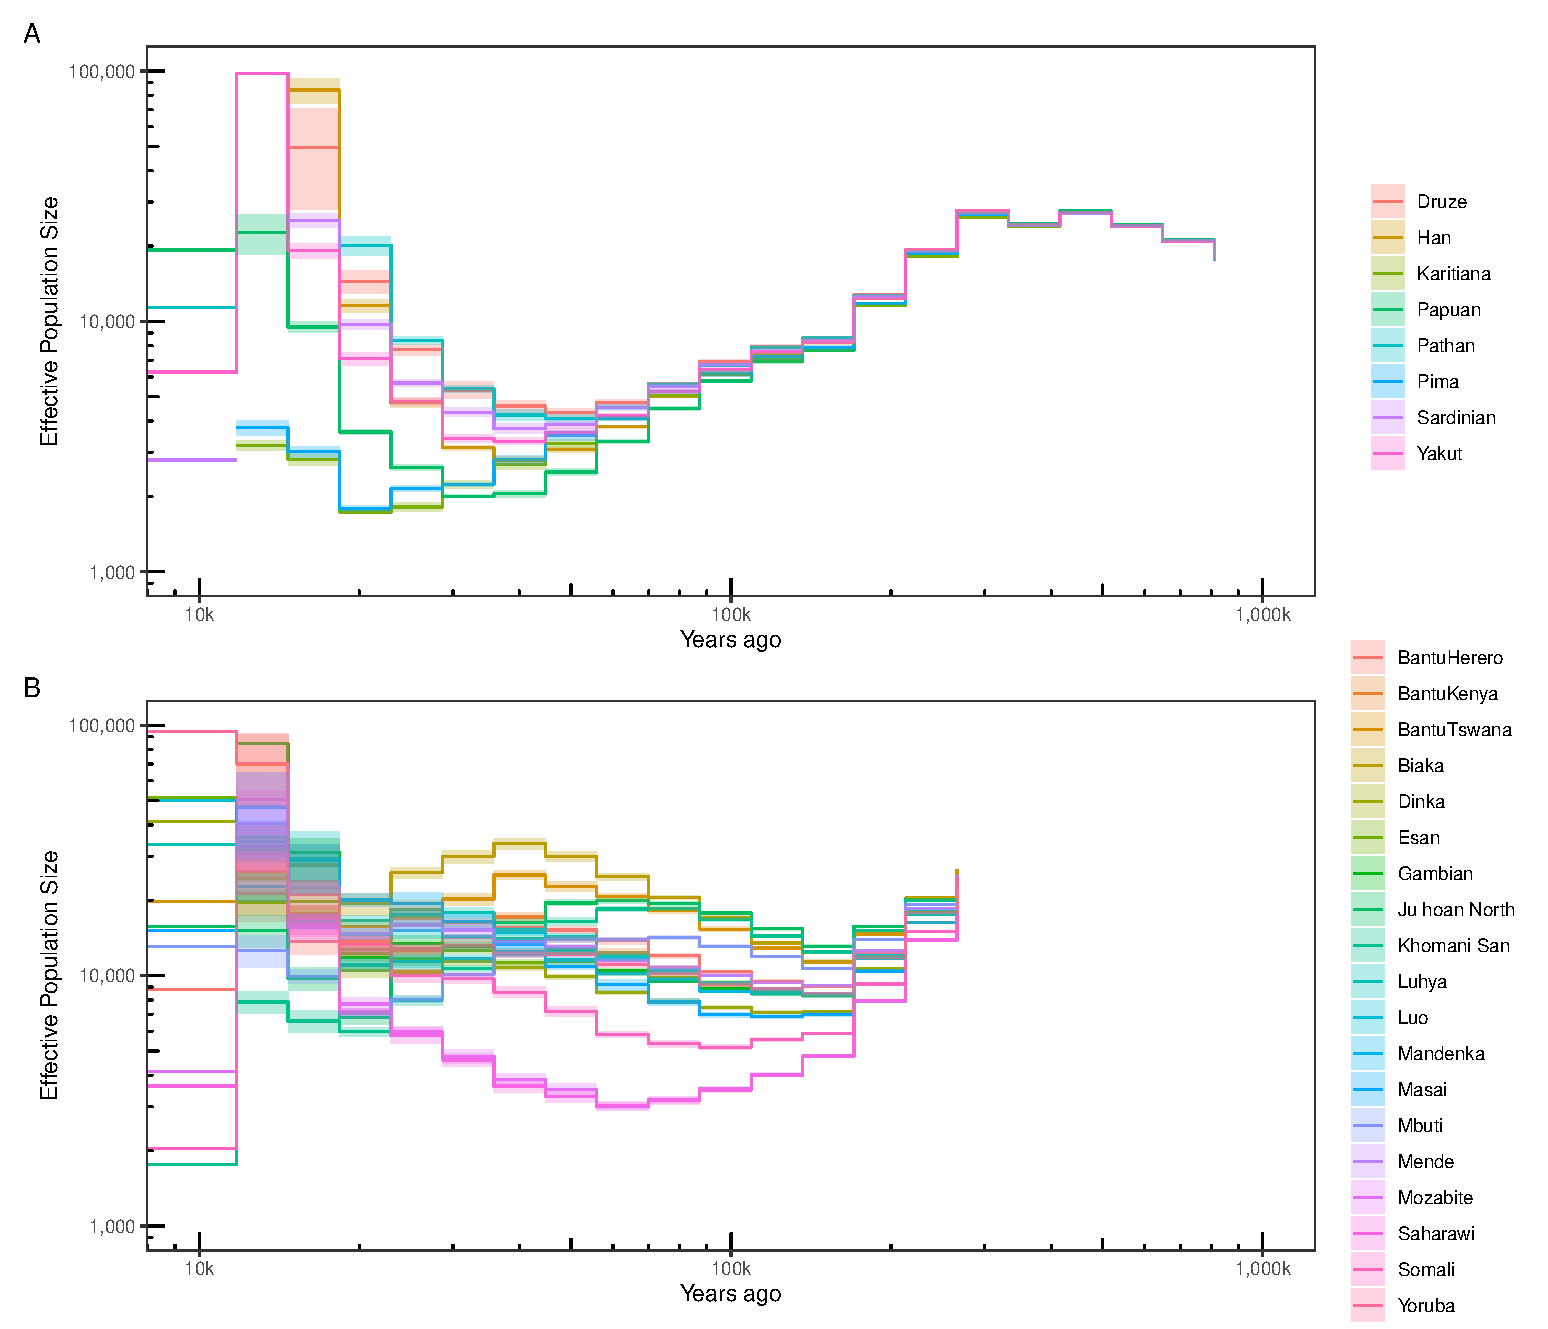
\includegraphics[width=\textwidth]{plot/individual_populations_averaged.pdf}
    \caption{\textbf{Estimates of individual population sizes incorporating directional migration.} Using {\tt SMCSMC} the effective population size of global populations in the Simons Genome Diversity Panel is inferred while simultaneously fitting directional migration estimates. Averages are plotted by epoch, with shaded regions denoting the standard deviation. {\bf a.} Estimates of Eurasian population sizes when averaged over Eurasian donor populations. This analysis uses the eight Eurasian populations matched to HGDP populations averaged over the four matched African populations. B. Estimates of African population sizes when averaged over Eurasian recipient populations. This analysis uses the three donor Eurasian populations used for the majority of the analyses in the main text (French, Han, and Papuan) along with the given African populations. Before approximately 250kya, the populations share the same population size within the model, and are not plotted. 10,000 particles are used to approximate the ancestral recombination graph in the SMCSMC particle filter and 15 iterations are used to update demographic parameter values. }
    \label{fig:individual_pop_sizes}
\end{figure}
\newpage


%S8-S10
\clearpage
\begin{figure}
	\centering
	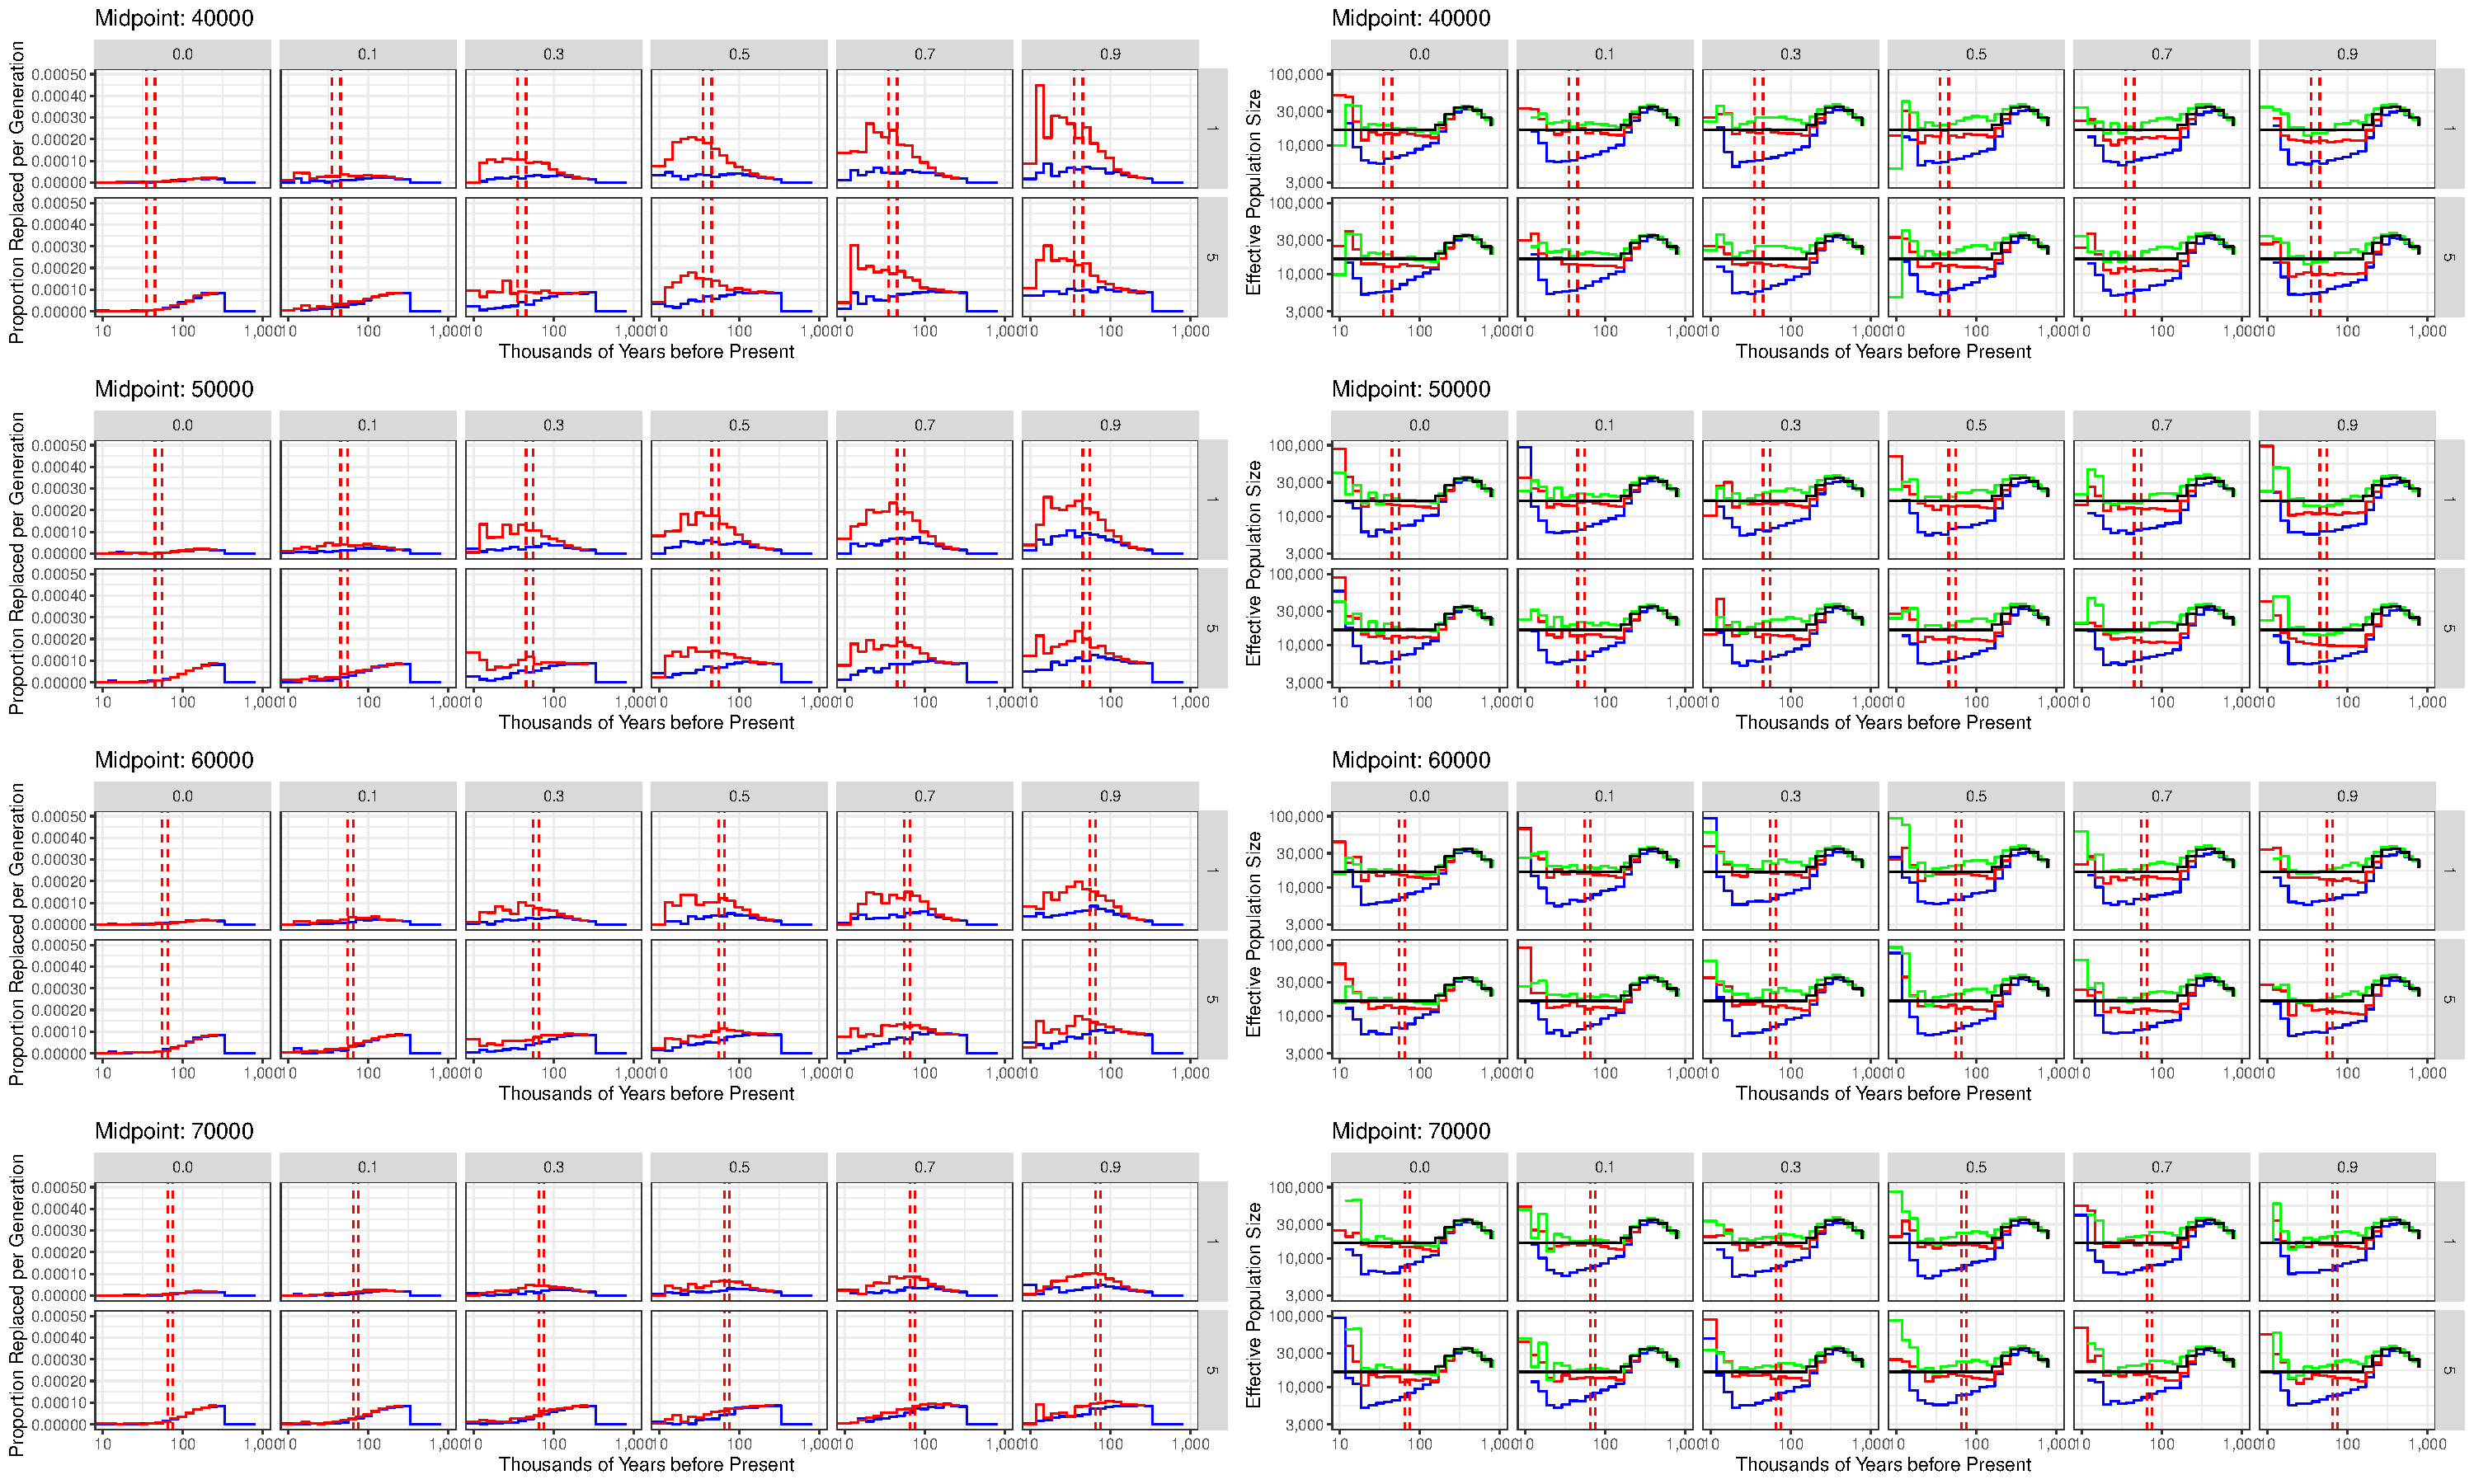
\includegraphics[width=\textwidth]{plot/backward_different_starts.pdf}
	\caption{{\bf Simulated migration backwards from effectively Eurasian to effectively African populations.} One gigabase of simulated sequence data was generated with {\tt SCRM} for two diploid individuals from different populations using a 100kb sliding window approximation of the coalescent with recombination and a demographic model similar to Eurasians and Africans specified in Supplemental section \ref{simproc}. The timing, representing the midpoint of a 10ky migration episode, and the integrated migration fraction (IMF) were systematically varied. In this scenario, only backwards migration was simulated. The left panel displays the recovered directional migration, with red lines representing migration backwards from Eurasia and blue representing migration forwards to Eurasia. The timing of the migration episode is demarcated with dotted red lines. The right panel displays the inferred effective population size of both populations. Additionally, the effective population size of the African-like population was modelled separately, without simultaneously inferring migration. 5000 particles were used in the {\tt SMCSMC} particle filter to approximate the ancestral recombination graph and 5 iterations of variational Bayesian inference were used to updated demographic parameter values.}
	\label{fig:backsim}
\end{figure}

\clearpage
\begin{figure}
	\centering
	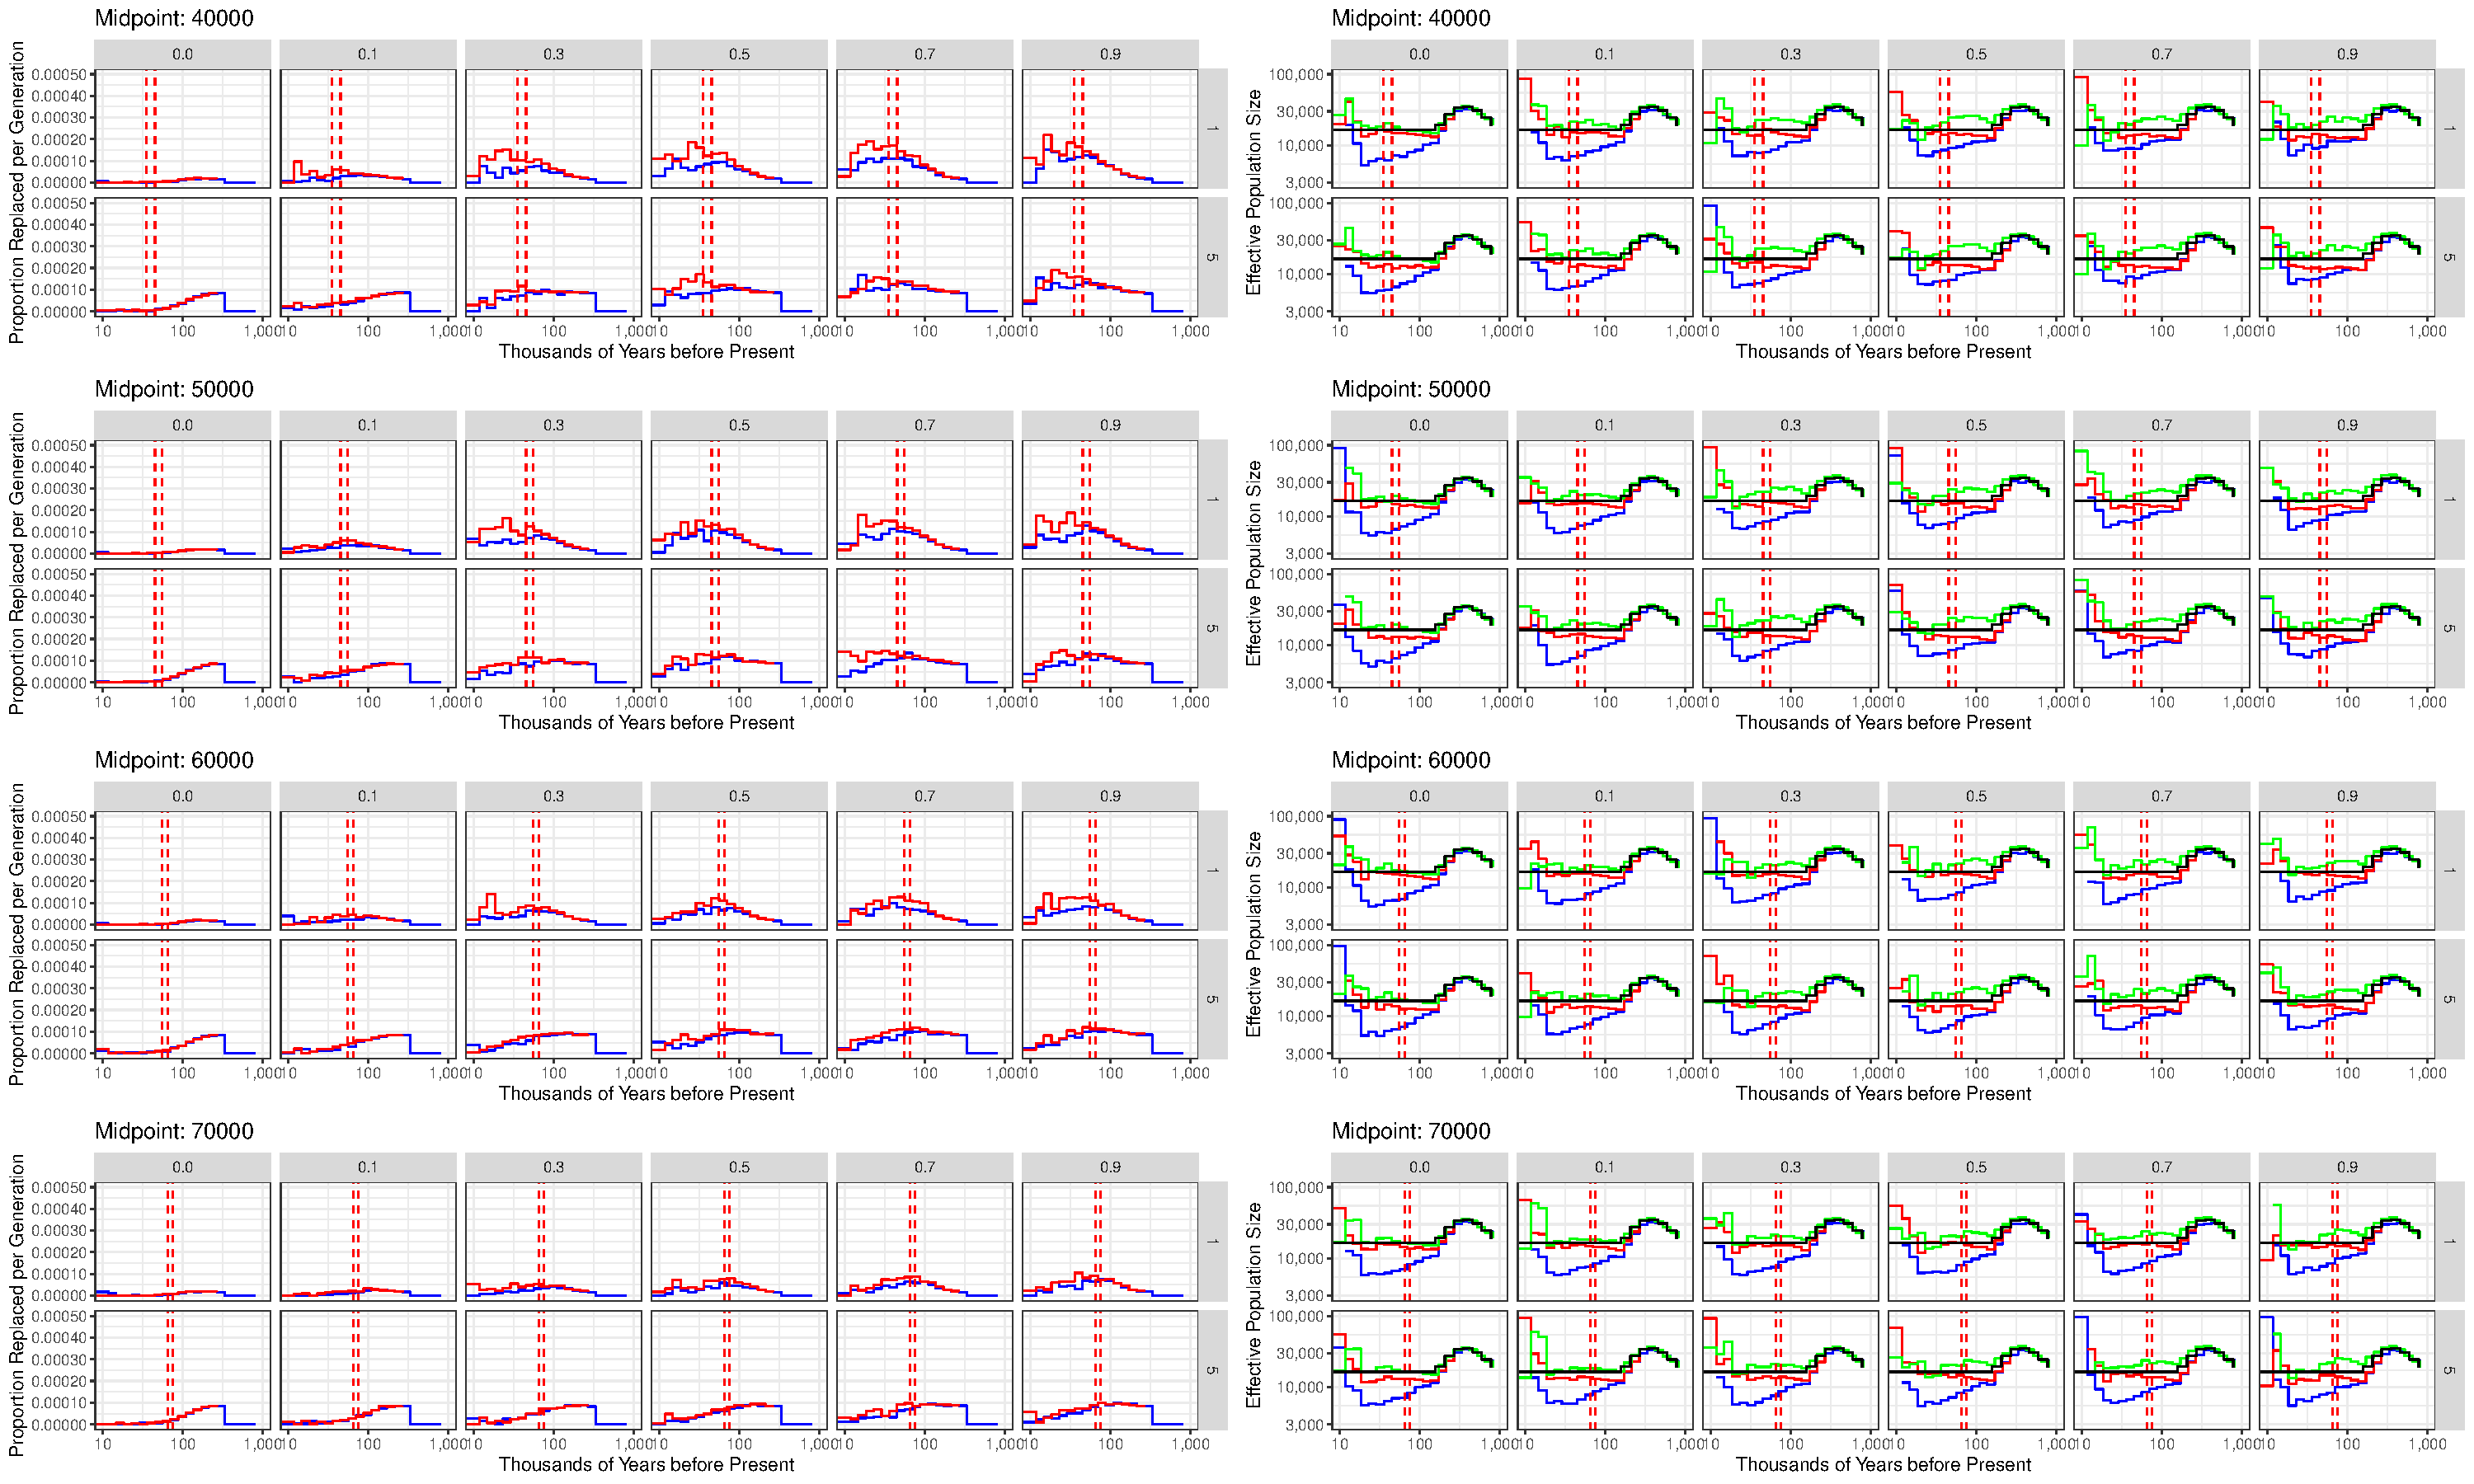
\includegraphics[width=\textwidth]{plot/bidirectional_different_starts.pdf}
	\caption{{\bf Simulated bidirectional migration between effectively Eurasian and effectively African populations.} One gigabase of simulated sequence data was generated with {\tt SCRM} for two diploid individuals from different populations using a 100kb sliding window approximation of the coalescent with recombination and a demographic model similar to Eurasians and Africans specified in Supplemental section \ref{simproc}. The timing, representing the midpoint of a 10ky migration episode, and the integrated migration fraction (IMF) were systematically varied. In this scenario, migration between these two populations was simulated with equal rates. The left panel displays the recovered directional migration, with red lines representing migration backwards from Eurasia and blue representing migration forwards to Eurasia. The timing of the migration episode is demarcated with dotted red lines. The right panel displays the inferred effective population size of both populations. Additionally, the effective population size of the African-like population was modelled separately, without simultaneously inferring migration. 5000 particles were used in the {\tt SMCSMC} particle filter to approximate the ancestral recombination graph and 5 iterations of variational Bayesian inference were used to updated demographic parameter values.}
	\label{fig:bisim}
\end{figure}

\clearpage
\begin{figure}
	\centering
	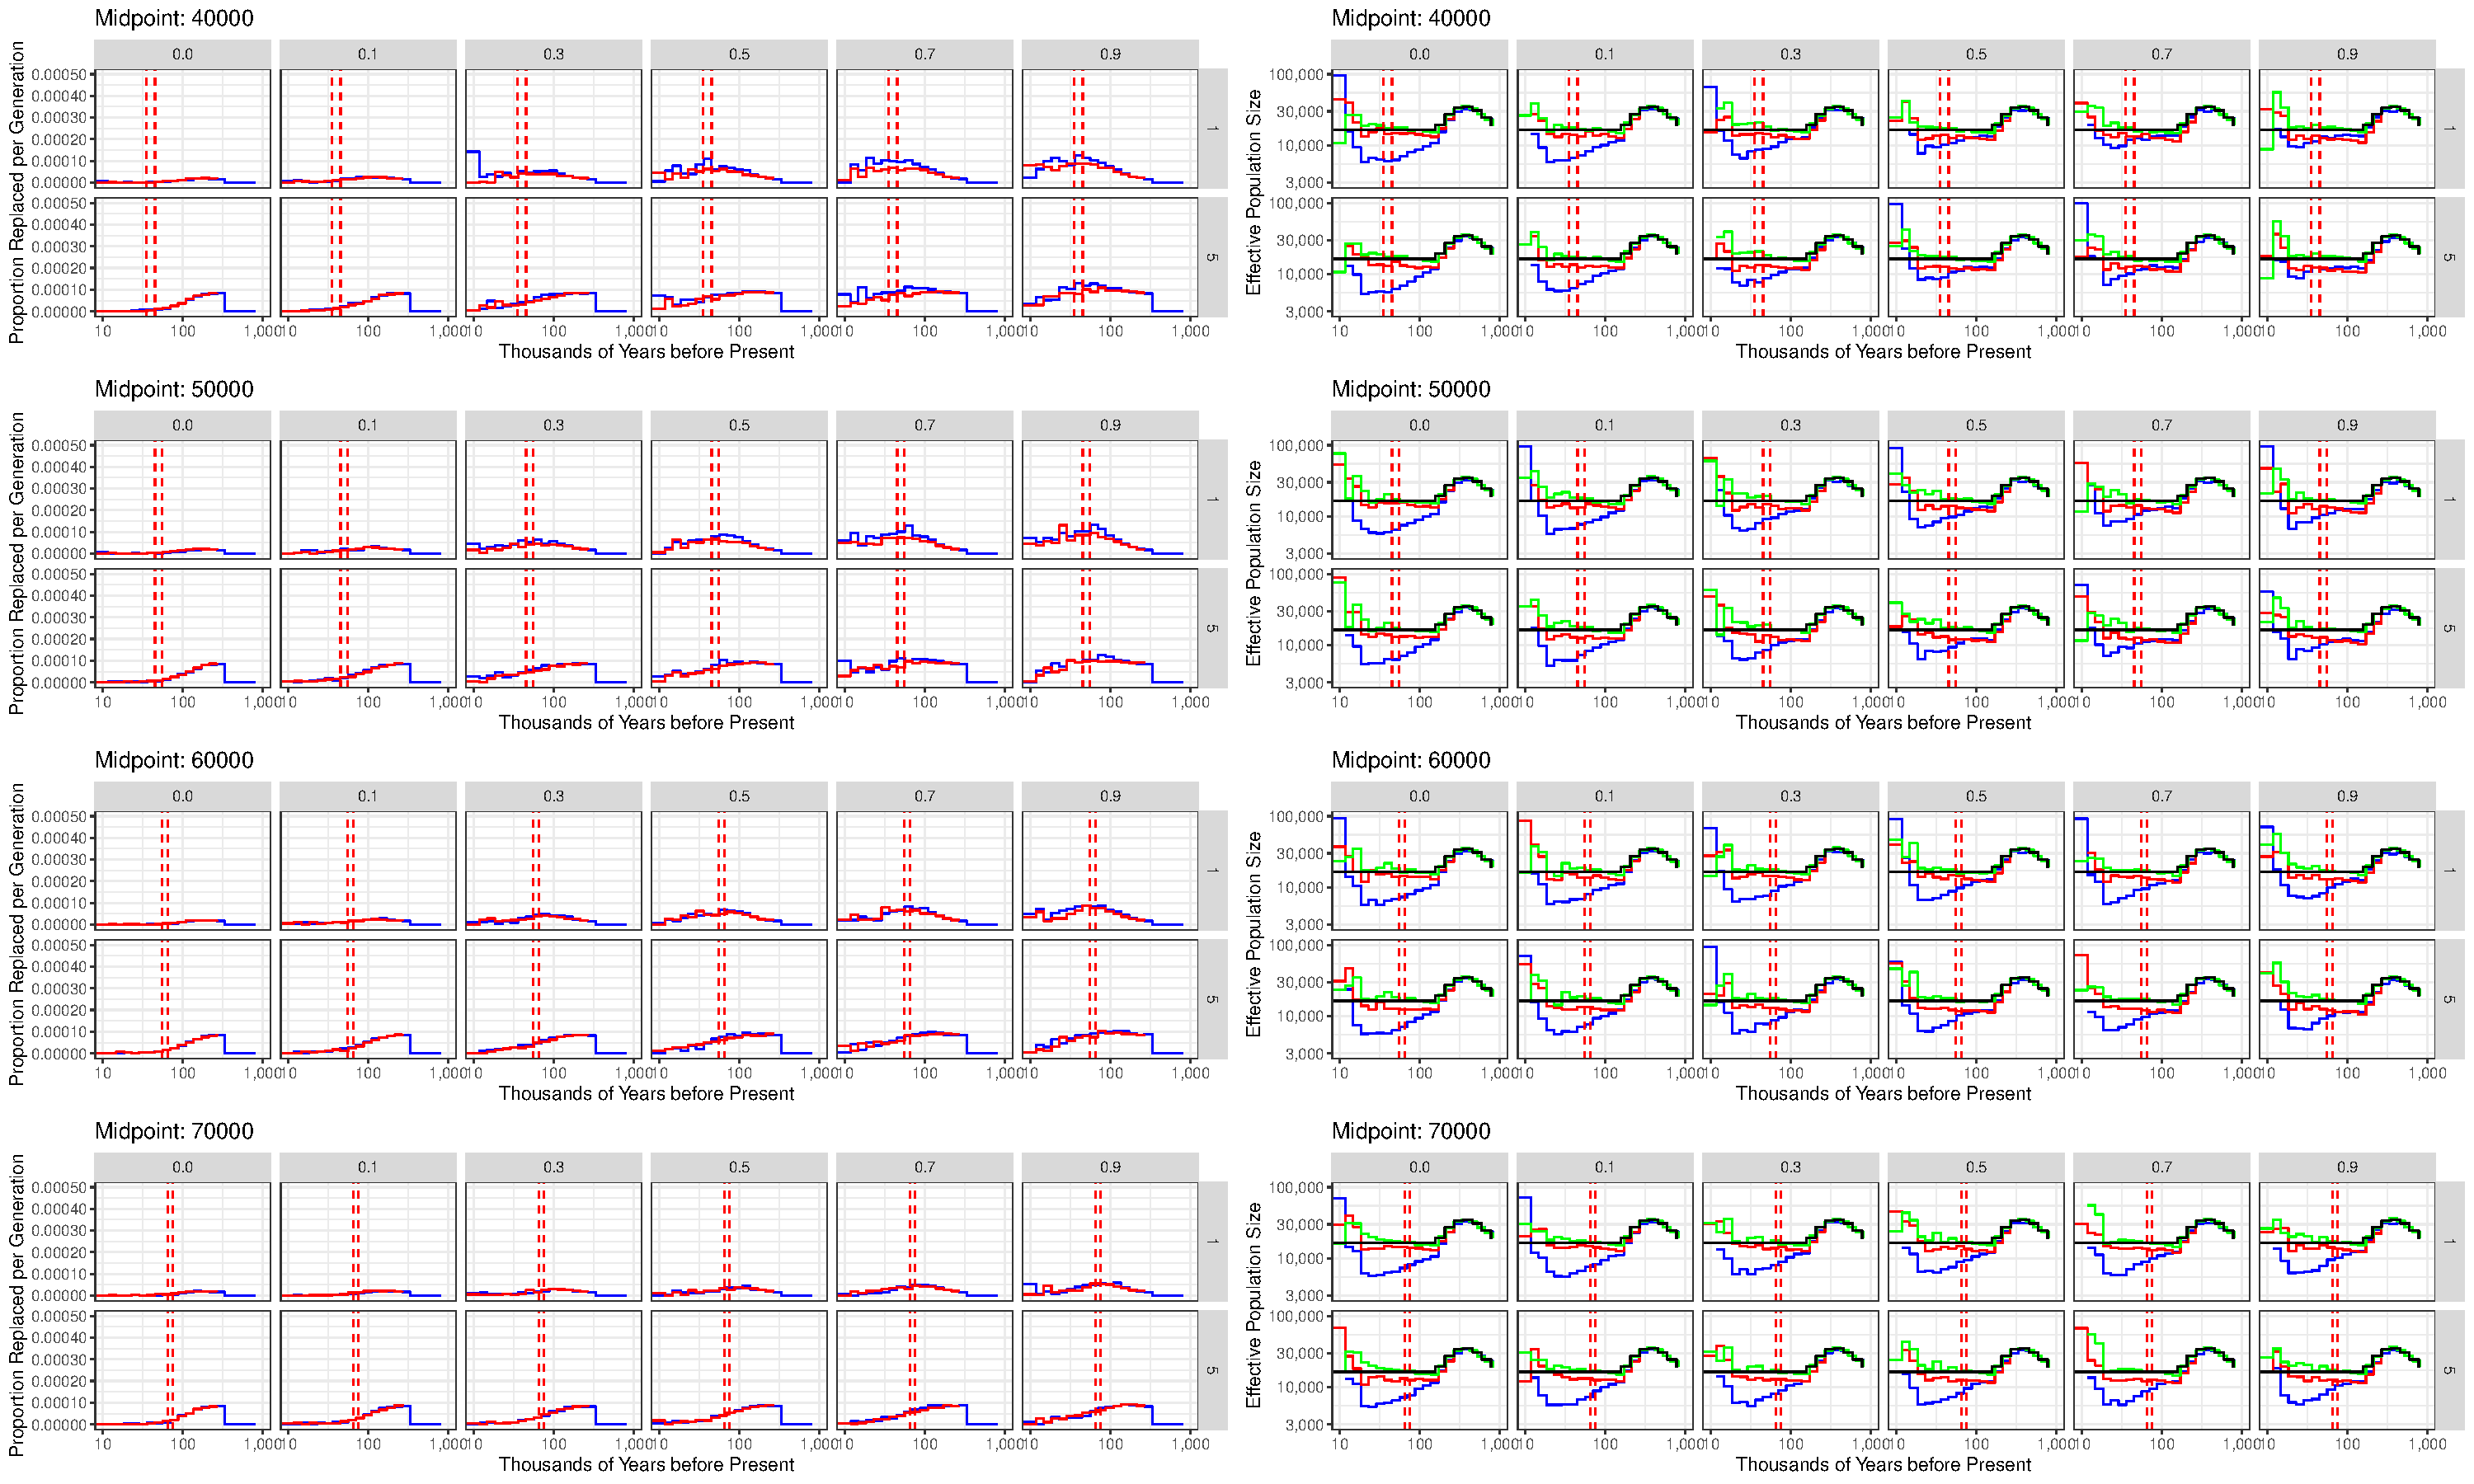
\includegraphics[width=\textwidth]{plot/forward_different_starts.pdf}
	\caption{{\bf Simulated migration forwards from effectively African to effectively Eurasian populations.} One gigabase of simulated sequence data was generated with {\tt SCRM} for two diploid individuals from different populations using a 100kb sliding window approximation of the coalescent with recombination and a demographic model similar to Eurasians and Africans specified in Supplemental section \ref{simproc}. The timing, representing the midpoint of a 10ky migration episode, and the integrated migration fraction (IMF) were systematically varied. In this scenario, only forwards migration was simulated. The left panel displays the recovered directional migration, with red lines representing migration backwards from Eurasia and blue representing migration forwards to Eurasia. The timing of the migration episode is demarcated with dotted red lines. The right panel displays the inferred effective population size of both populations. Additionally, the effective population size of the African-like population was modelled separately, without simultaneously inferring migration. 5000 particles were used in the {\tt SMCSMC} particle filter to approximate the ancestral recombination graph and 5 iterations of variational Bayesian inference were used to updated demographic parameter values.}
	\label{fig:fwdsim}
\end{figure}
%S6






\begin{figure}
    \centering
    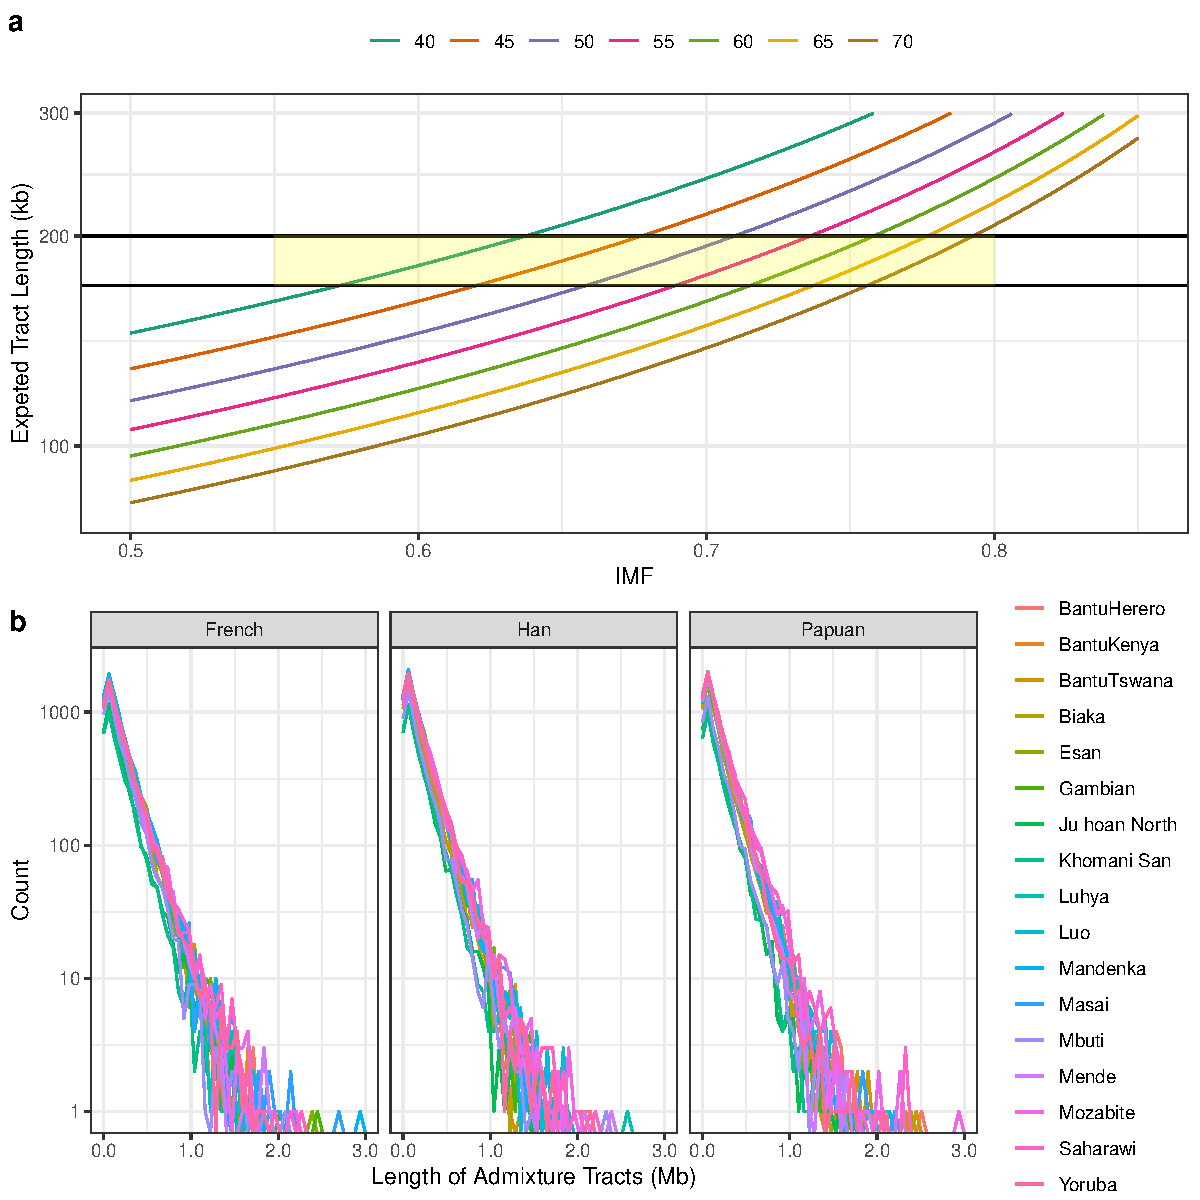
\includegraphics[width=\textwidth]{plot/both_length.pdf}
    \caption{ {\bf Analysis of the length of putatively migrated segments}. {\bf a.} Theoretical length distribution of admixture tract rate parameter under varying migration and admixture timing assuming that $L = ((1-m)r(T-1))^-1$, given $L$ length, $m$ symmetrical migration rate, $r$ recombination rate in events per nucleotide, and $T$ time in generations \cite{Liang953}. Shaded region denotes empirical range (with San at the bottom end, and Yoruban at the top end, Supplemental Table \ref{table:lengths}) of fragments observed in the Simons Genome Diversity Panel. {\bf b.} Following the reconstruction of the ancestral recombination graph using different African and non-African individuals using the {\tt SMCSMC} particle filter, we use a sample of the posterior distribution of marginal trees to reconstruct putatively migrated segments (see Methods). We plot the length distribution of admixture tracts between individuals in the SGDP using 50 bins. Length is given in megabases (Mb). Isolated from {\tt SMCSMC} estimated ancestral recombination graphs. Migration rate is given in terms of proportion of the sink population replaced per generation. }
    \label{fig:length}
\end{figure}




\begin{figure}
    \centering
    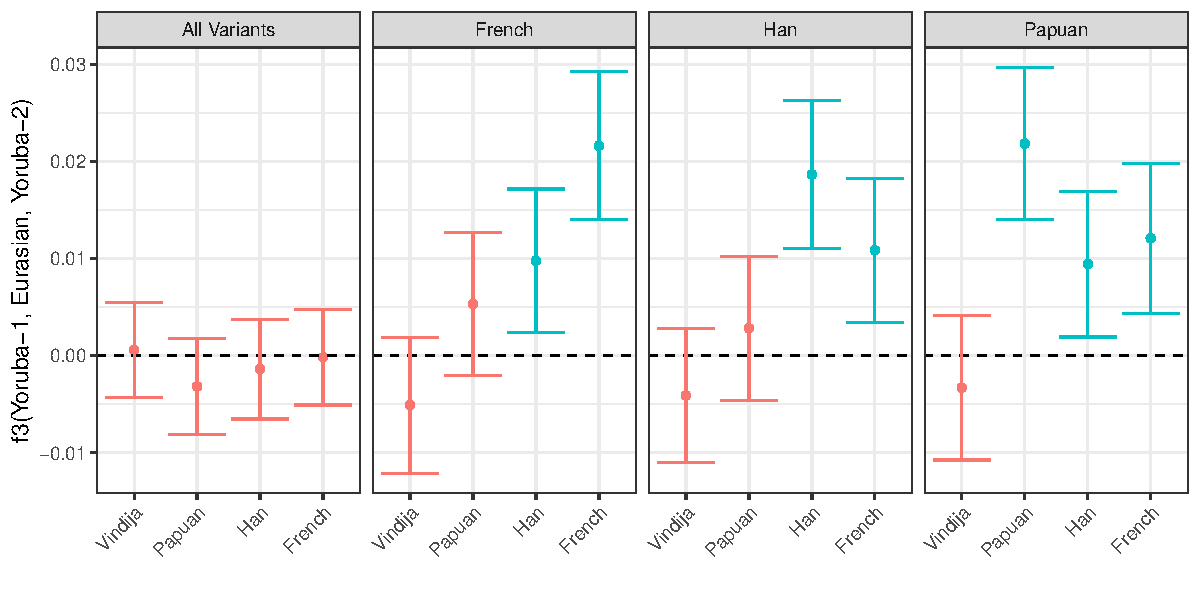
\includegraphics[width = \textwidth]{plot/f3.pdf}
    \caption{ {\bf $f_3$ statistics show evidence for shared drift with Eurasians}. Following the reconstruction of putatively migrated segments from the inferred ancestral recombination graph, we use the Reich Human Origins data set to investigate admixture using drift statistics using {\tt ADMIXTOOLS} and {\tt admixr} (see URLs). Tests are separated into all markers, and those ascertained through {\tt SMCSMC} runs with the French, Han, and Papuans as a comparison Eurasian group. The $f_3$ statistics estimate is plotted, along with 95\% C.I. computed via a block jackknife. Statistics which are significantly larger than zero are coloured blue, indicating shared drift.}
    \label{fig:f3}
\end{figure}

\begin{figure}
    \centering
    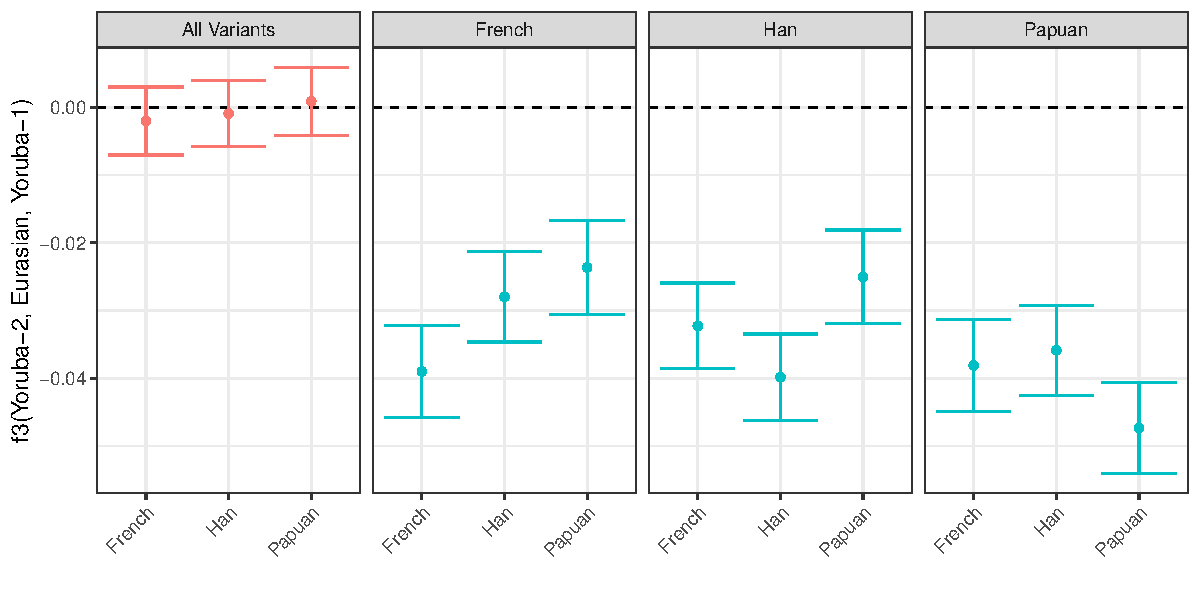
\includegraphics[width=\textwidth]{plot/f3_admix.pdf}
    \caption{{\bf $f_3$ statistics show evidence for Eurasian admixture}. Following the reconstruction of putatively migrated segments from the inferred ancestral recombination graph, we use the Reich Human Origins data set to investigate admixture using drift statistics using {\tt ADMIXTOOLS} and {\tt admixr} (see URLs). Tests are separated into all markers, and those ascertained through {\tt SMCSMC} runs with the French, Han, and Papuans as a comparison Eurasian group. The $f_3$ statistics estimate is plotted, along with 95\% C.I. computed via a block jackknife. Statistics which are significantly less than zero indicate statistical evidence for admixture, and are coloured blue.}
    \label{fig:f3_admix}
\end{figure}

\begin{figure}[ht]
	\centering
	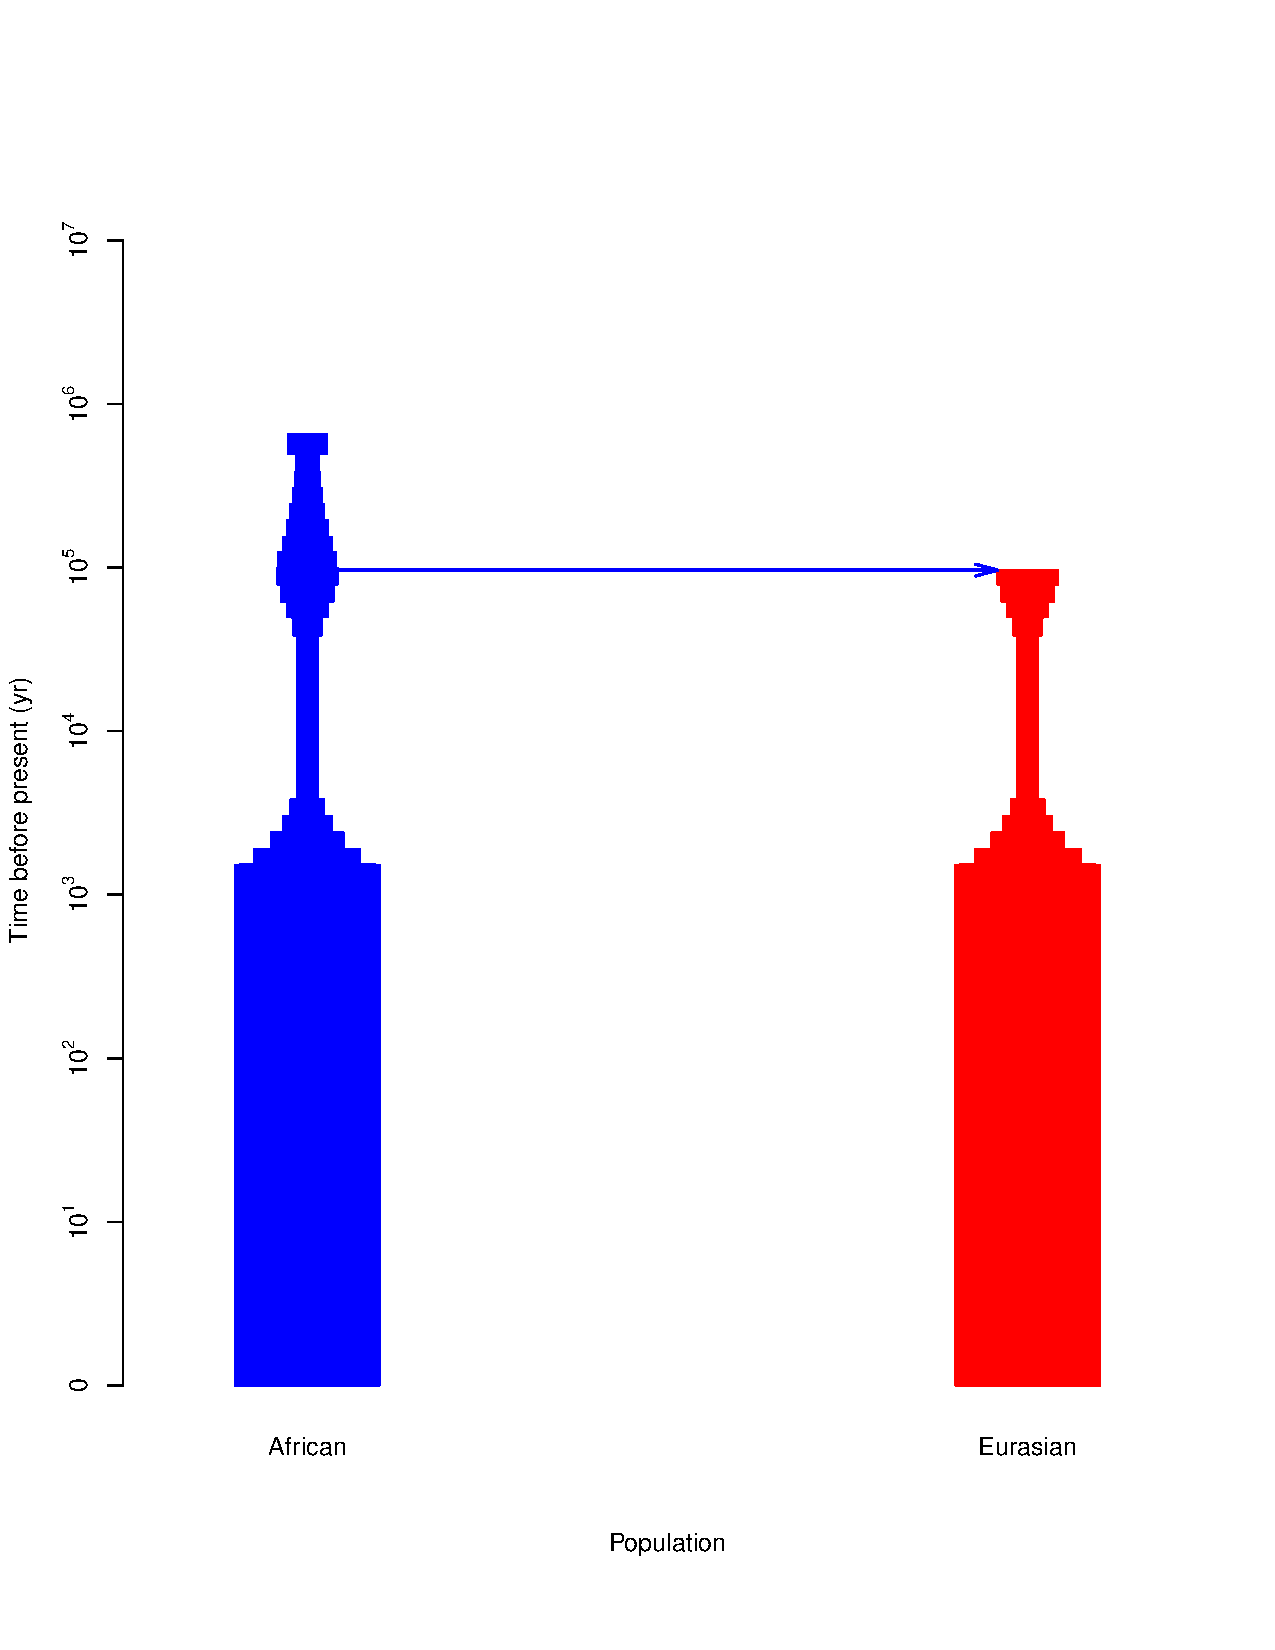
\includegraphics[width=0.5\textwidth]{plot/dem_smc2.pdf}
	\caption{Demographic model used as initialisation for {\tt SMCSMC} analysis visualised using PopDemog \cite{Zhou2018}.}
	\label{smc2demog}
\end{figure}
\newpage

%\begin{figure}
%    \centering
%    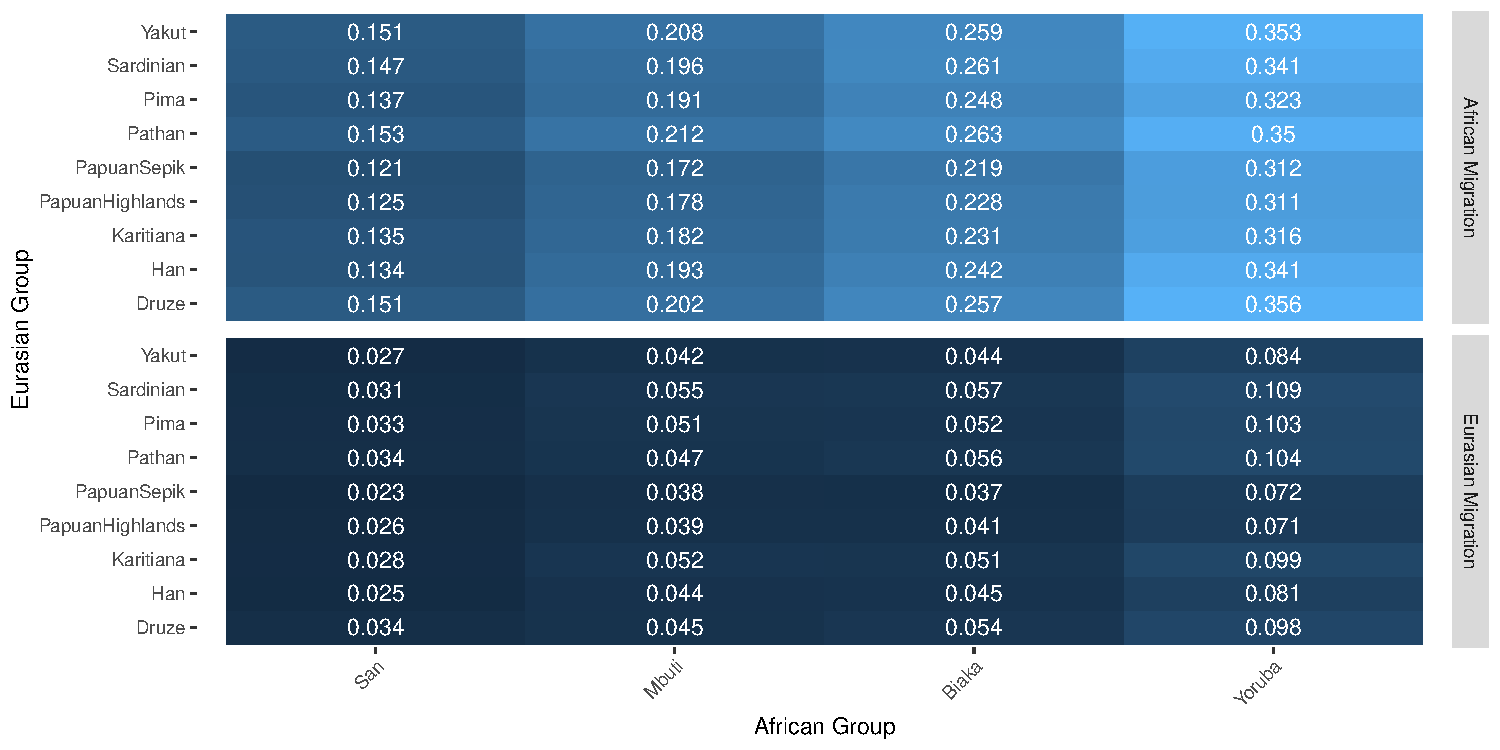
\includegraphics[width = \textwidth]{plot/imf_hgdp.pdf}
%    \caption{Integrated migration fraction over the period 30--70kya in the physically phased subset of the Human Genome Diversity Panel. Displayed are values averaged over three technical replicates to reduce the effect of stochastic sampling.}
%    \label{fig:hgdp_imf}
%\end{figure}


\begin{figure}
	\centering
	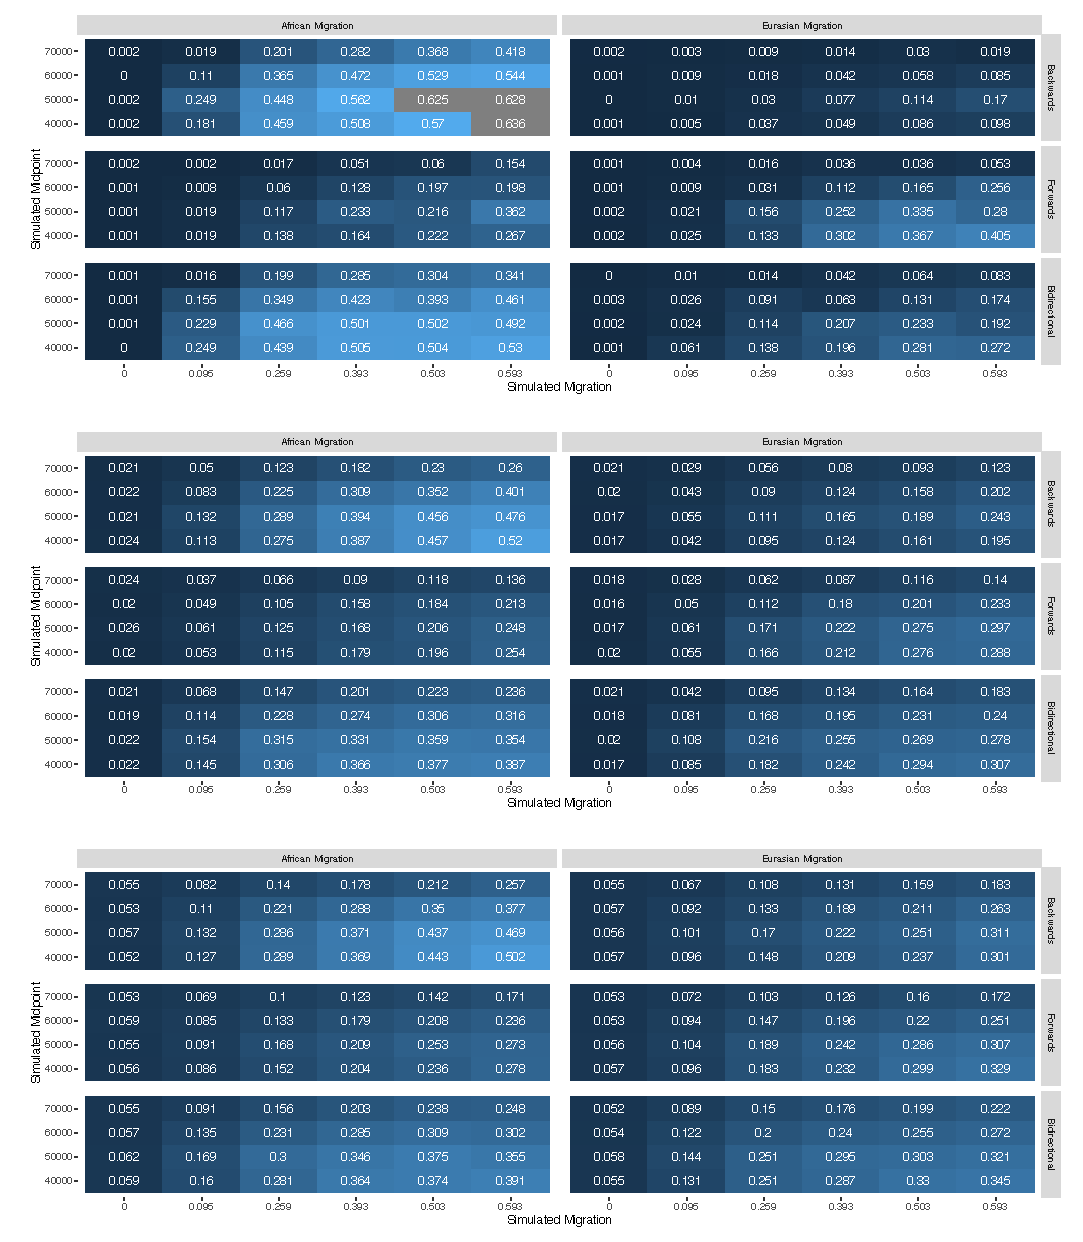
\includegraphics[width=\textwidth]{plot/all_integrated_sims.pdf}
	\caption{ {\bf Integrated migration fraction (IMF) in the last 100ky for three cases of simulated demography shown in Figures \ref{fig:backsim}, \ref{fig:bisim}, and \ref{fig:fwdsim}.} Simulations were performed as per Supplemental Section \ref{simproc} with an additional parameter for the initial migration rate used to initialise the {\tt SMCSMC} particle filter. The timing and IMF simulated are as per the aforementioned figures. From top to bottom, inference was initiated with 0, 1, and 5 4$N_0$ population replacement per generation in the specified direction (backwards, bidirectionally, and forwards).}
	\label{fig:intsim}
\end{figure}

\begin{figure}
	\centering
	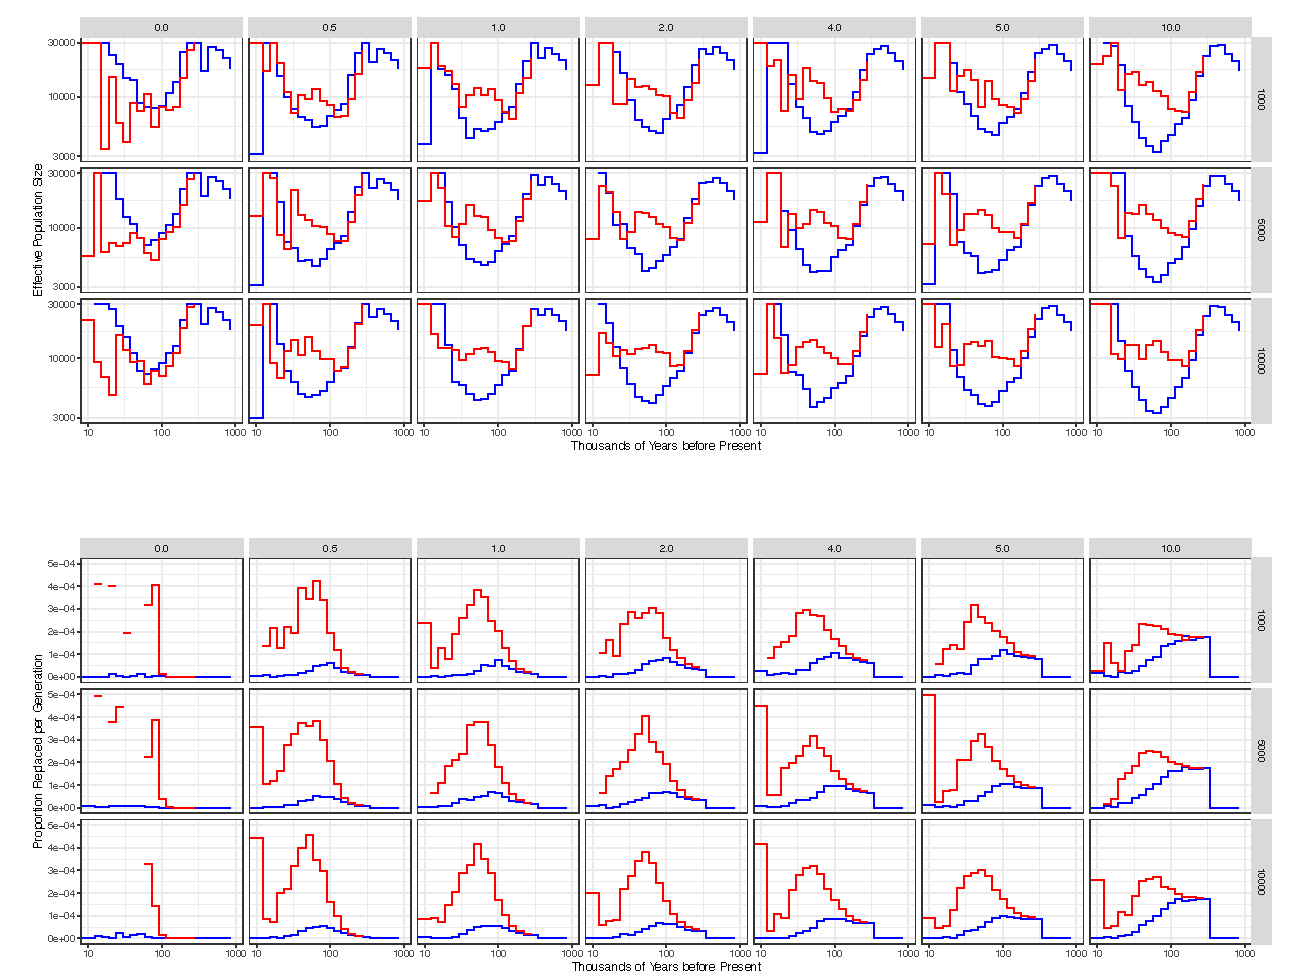
\includegraphics[width=\textwidth]{plot/yri_dif_migs.pdf}
	\caption{ {\bf The effect of initial migration parameter on demographic inference.} Effective population size and migration history of a Yoruban ({\tt S\_Yoruba-1}) and a French ({\tt S\_French-1}) individual from the Simons Genome Diversity panel were modelled with {\tt SMCSMC}. The initial migration proportion, in units of 4 $N_0$ proportion of the population replaced per generation was varied along the X axis, while the number of particles is varied along the Y. 10 iterations of variational Bayes was used for parameter inference, while 5000 particles were used infer the ancestral recombination graph.}
	\label{init_yri}
\end{figure}

\begin{figure}[hb]
    \centering
    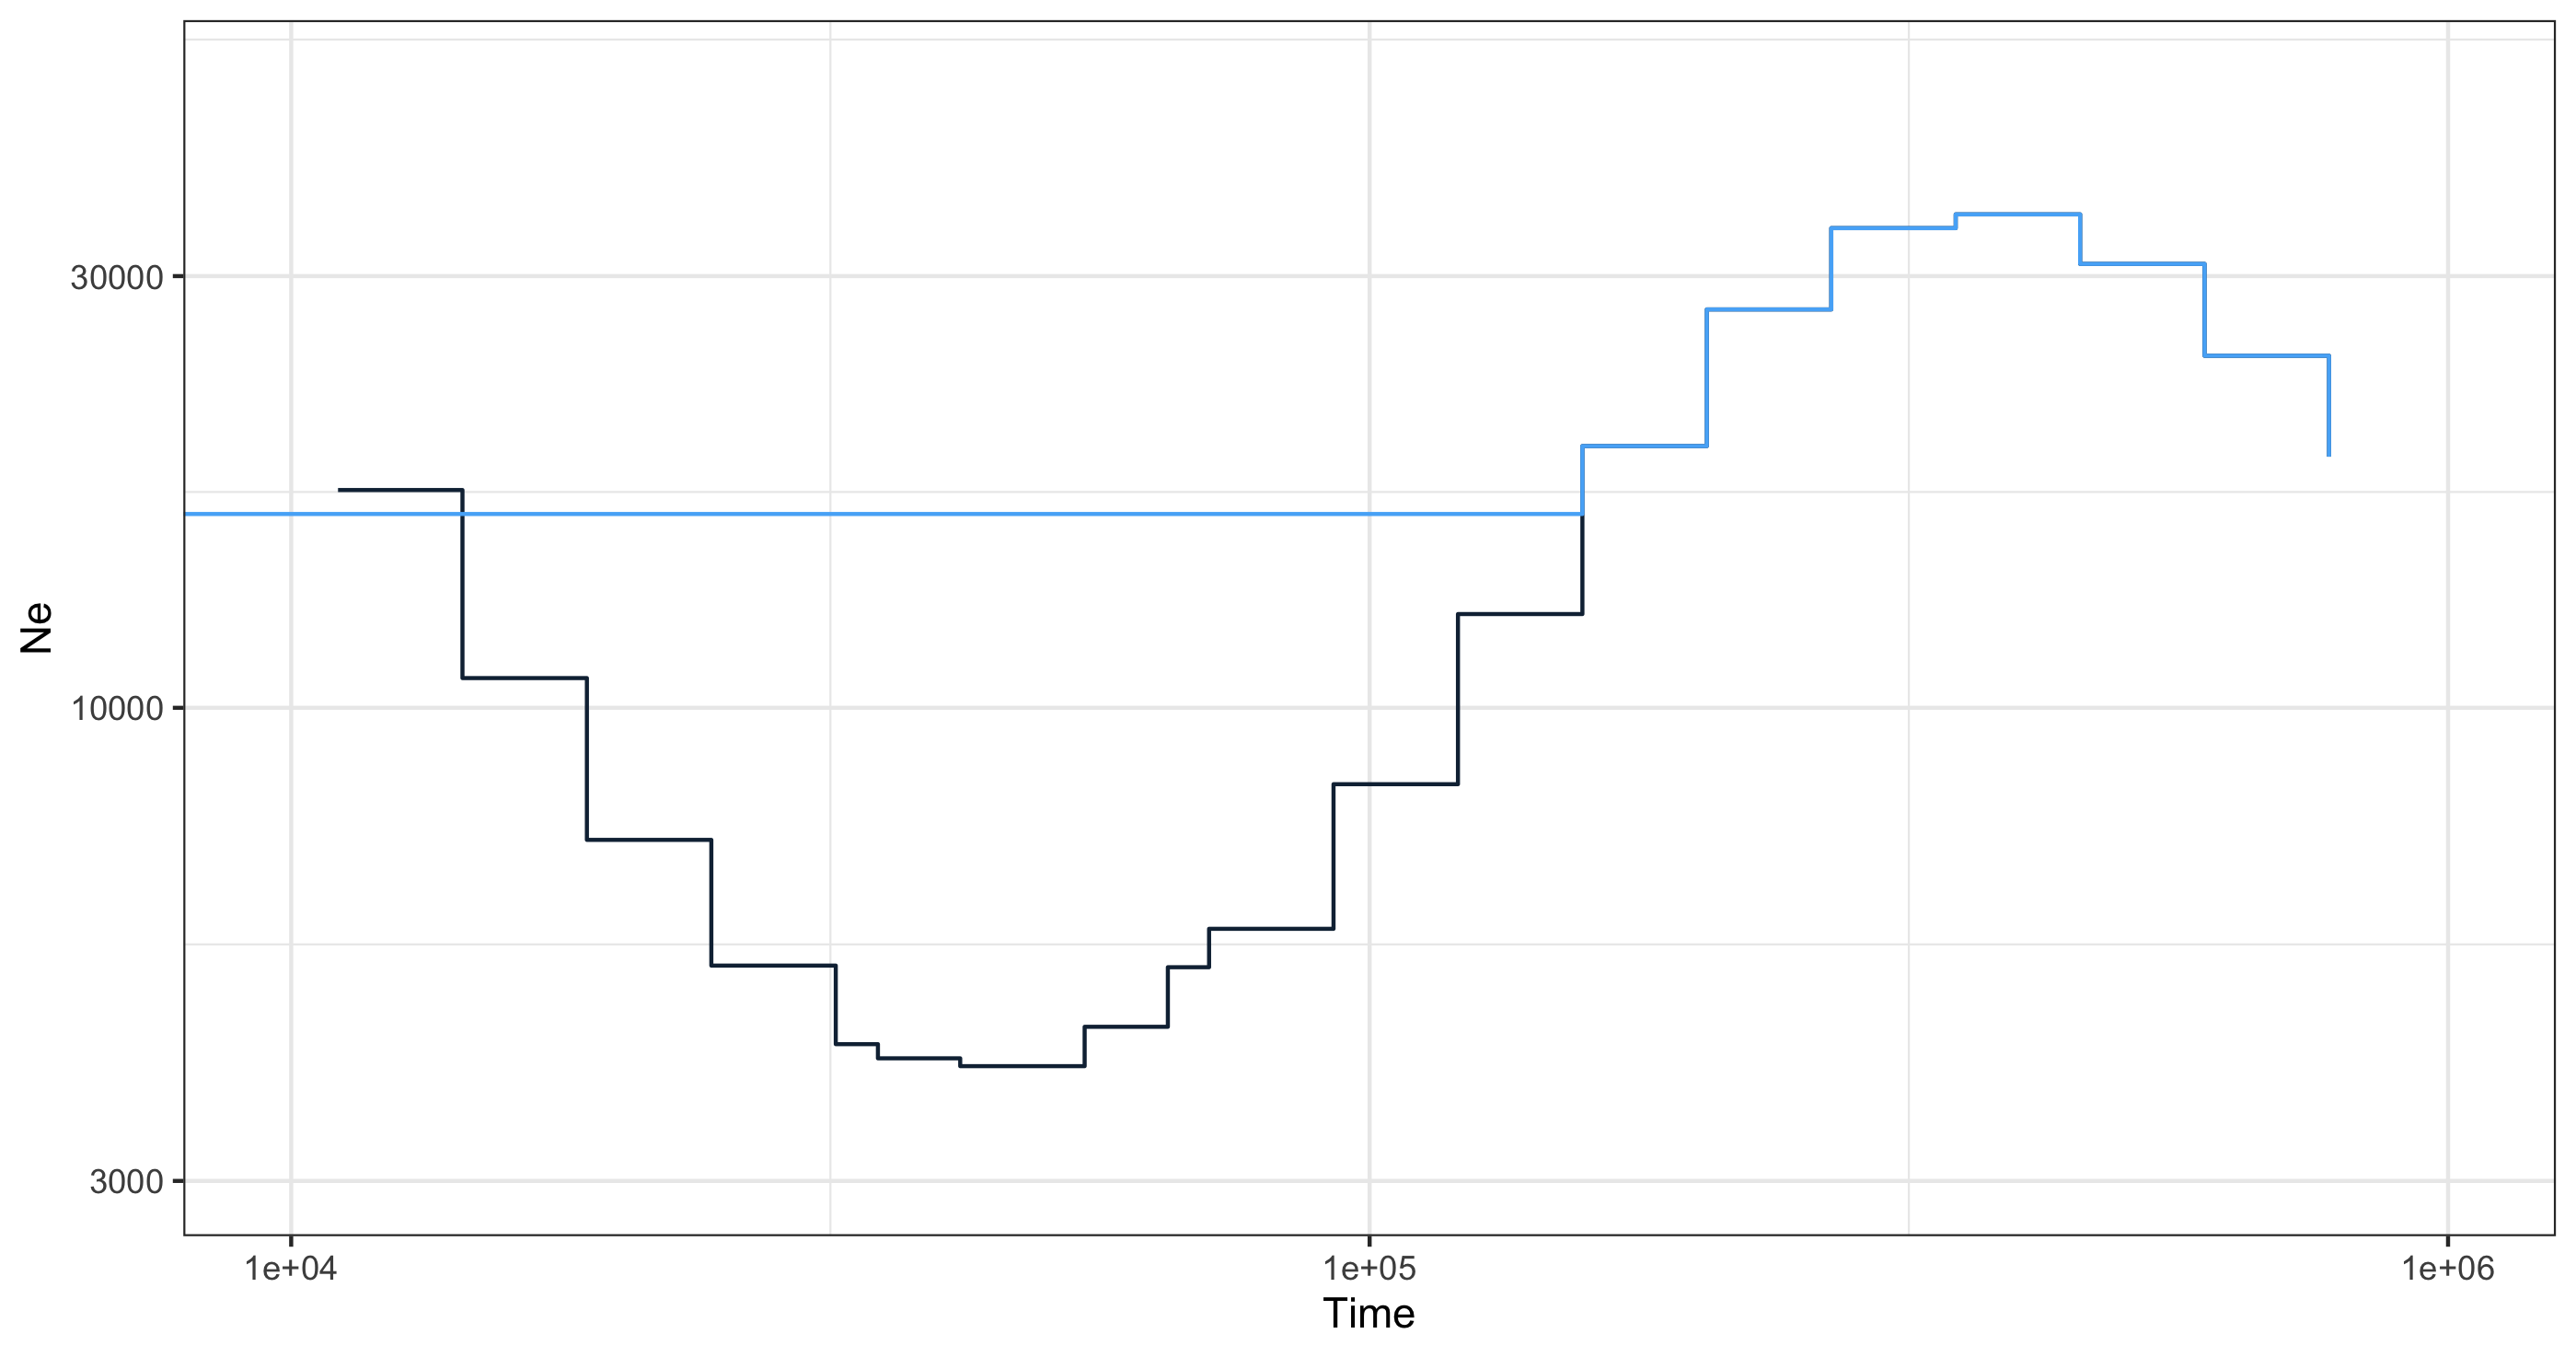
\includegraphics[width = 0.5\linewidth]{plot/demographic_model.png}
    \caption{{\bf Effective Population size model used for simulations.} Following the simulation procedure in Supplemental Section \ref{simproc}, the population size model is plotted per epoch, with the effectively African population plotted in blue and the effectively non-African population in black. }
    \label{fig:dem}
\end{figure}



\clearpage

\section{Supplemental Tables}

% latex table generated in R 3.5.3 by xtable 1.8-3 package
% Wed Jan 22 11:49:06 2020
\begin{table}[ht]
\centering
\begin{tabular}{llll}
  \hline
Language Family & Partner Population & Mean AFR IMF (SD) & Mean EUR IMF (SD) \\ 
  \hline
Afroasiatic & All & 0.477(0.015) & 0.176(0.038) \\ 
  Afroasiatic & French & 0.477(0.006) & 0.207(0.044) \\ 
  Afroasiatic & Han & 0.492(0.01) & 0.168(0.032) \\ 
  Afroasiatic & Papuan & 0.462(0.011) & 0.153(0.024) \\ 
  Khoesan & All & 0.209(0.013) & 0.044(0.006) \\ 
  Khoesan & French & 0.217(0.007) & 0.051(0.003) \\ 
  Khoesan & Han & 0.217(0.002) & 0.042(0) \\ 
  Khoesan & Papuan & 0.193(0.006) & 0.04(0) \\ 
  Niger-Kordofanian & All & 0.352(0.04) & 0.088(0.017) \\ 
  Niger-Kordofanian & French & 0.36(0.039) & 0.102(0.015) \\ 
  Niger-Kordofanian & Han & 0.363(0.04) & 0.083(0.013) \\ 
  Niger-Kordofanian & Papuan & 0.334(0.038) & 0.078(0.013) \\ 
  Nilo-Saharan & All & 0.405(0.033) & 0.107(0.016) \\ 
  Nilo-Saharan & French & 0.414(0.037) & 0.123(0.016) \\ 
  Nilo-Saharan & Han & 0.417(0.036) & 0.106(0.01) \\ 
  Nilo-Saharan & Papuan & 0.385(0.029) & 0.093(0.008) \\ 
   \hline
\end{tabular}
\caption{{\bf Integrated Migration Fraction (IMF) in either direction averaged over African language groups.} {\tt SMCSMC} was used as in Supplemental Section \ref{data-analysis} to infer directional migration and effective population size between populations in the Simons Genome Diversity Project. The total migration between each African and non-African population was integrated in the epoch 30--70kya (see Methods) and averaged over language family. Abbreviations: Integrated Migration Fraction (IMF), Stanard Deviation (SD), EUR (Eurasian), AFR (African)} 
\label{average_sgdp_migration_table}
\end{table}


\begin{table}[ht]
\centering
\begin{tabular}{rrrrr}
  \hline
 & Estimate & Std. Error & t value & Pr($>$$|$t$|$) \\ 
  \hline
(Intercept) & 0.3807 & 0.0036 & 105.42 & 1.79e-47 \\ 
  Papuan & -0.0271 & 0.0017 & -15.60 & 7.44e-18 \\ 
  BantuKenya & 0.0051 & 0.0050 & 1.02 & 3.16e-01 \\ 
  BantuTswana & -0.0410 & 0.0050 & -8.13 & 9.49e-10 \\ 
  Biaka & -0.0598 & 0.0050 & -11.87 & 3.53e-14 \\ 
  Dinka & 0.0160 & 0.0050 & 3.17 & 3.05e-03 \\ 
  Esan & -0.0016 & 0.0050 & -0.32 & 7.51e-01 \\ 
  Gambian & -0.0073 & 0.0050 & -1.44 & 1.58e-01 \\ 
  Ju hoan North & -0.1603 & 0.0050 & -31.79 & 1.82e-28 \\ 
  Khomani San & -0.1653 & 0.0050 & -32.80 & 5.96e-29 \\ 
  Luhya & 0.0118 & 0.0050 & 2.34 & 2.46e-02 \\ 
  Luo & 0.0123 & 0.0050 & 2.45 & 1.94e-02 \\ 
  Mandenka & 0.0032 & 0.0050 & 0.63 & 5.34e-01 \\ 
  Masai & 0.0719 & 0.0050 & 14.25 & 1.32e-16 \\ 
  Mbuti & -0.1171 & 0.0050 & -23.22 & 1.17e-23 \\ 
  Mende & -0.0071 & 0.0050 & -1.42 & 1.65e-01 \\ 
  Mozabite & 0.1060 & 0.0050 & 21.02 & 3.63e-22 \\ 
  Saharawi & 0.1097 & 0.0050 & 21.75 & 1.12e-22 \\ 
  Somali & 0.0995 & 0.0050 & 19.73 & 3.12e-21 \\ 
  Yoruba & -0.0013 & 0.0050 & -0.26 & 7.97e-01 \\ 
   \hline
\end{tabular}
\caption{{\bf Linear model predicting integrated migration fraction in the SGDP.} The integrated migration fraction (IMF) in the epoch 30--70 kya is obtained as per the Methods section in the Simons Genome Diversity Project.  A binary variable representing Papuan / not Papuan Eurasian donor and categorical variable representing African population were used to predict the IMF in a simple linear model. When adjusted for the different African populations, Papuans contribute less IMF than do other Eurasian partners (French and Han).} 
\label{sgdp:papuan_imf}
\end{table}

\begin{table}[ht]
\centering
\begin{tabular}{rrrrr}
  \hline
 & Estimate & Std. Error & t value & Pr($>$$|$t$|$) \\ 
  \hline
(Intercept) & 0.3392 & 0.0037 & 92.92 & 1.72e-39 \\ 
  Papuan & -0.0252 & 0.0042 & -5.95 & 1.43e-06 \\ 
  San & -0.1942 & 0.0050 & -38.94 & 6.85e-28 \\ 
  Mbuti & -0.1410 & 0.0050 & -28.27 & 1.07e-23 \\ 
  Biaka & -0.0883 & 0.0050 & -17.69 & 9.33e-18 \\ 
   \hline
\end{tabular}
\caption{ {\bf Linear model predicting integrated migration fraction in the HGDP.} The integrated migration fraction (IMF) in the epoch 30--70 kya is obtained as per the Methods section in the physically phased subset of the Human Genome Diversity Project.  A binary variable representing Papuan / not Papuan Eurasian donor and categorical variable representing African population were used to predict the IMF in a simple linear model. When adjusted for the different African populations, Papuans contribute less IMF than do other Eurasian partners (French and Han). } 
\label{hgdp:papuan_imf}
\end{table}

\begin{table}[ht]
\centering
\begin{tabular}{llrr}
  \hline
Language Family & Comparison Family & Mean Difference (95\% CI) & Adjusted P \\ 
  \hline
Niger-Kordofanian & Nilo-Saharan & -0.053 (-0.081--0.025) & 1.11e-03 \\ 
  Niger-Kordofanian & Khoesan & 0.143 (0.125-0.161) & 4.39e-14 \\ 
  Niger-Kordofanian & Afroasiatic & -0.125 (-0.142--0.107) & 1.67e-15 \\ 
  Nilo-Saharan & Niger-Kordofanian & 0.053 (0.025-0.081) & 1.11e-03 \\ 
  Nilo-Saharan & Khoesan & 0.196 (0.169-0.223) & 6.91e-09 \\ 
  Nilo-Saharan & Afroasiatic & -0.072 (-0.098--0.045) & 1.23e-04 \\ 
  Khoesan & Niger-Kordofanian & -0.143 (-0.161--0.125) & 4.39e-14 \\ 
  Khoesan & Nilo-Saharan & -0.196 (-0.223--0.169) & 6.91e-09 \\ 
  Khoesan & Afroasiatic & -0.268 (-0.284--0.252) & 3.62e-13 \\ 
  Afroasiatic & Niger-Kordofanian & 0.125 (0.107-0.142) & 1.67e-15 \\ 
  Afroasiatic & Nilo-Saharan & 0.072 (0.045-0.098) & 1.23e-04 \\ 
  Afroasiatic & Khoesan & 0.268 (0.252-0.284) & 3.62e-13 \\ 
  CAHG & Niger-Kordofanian & -0.084 (-0.119--0.049) & 1.18e-03 \\ 
   \hline
\end{tabular}
\caption{ {\bf Differences in African IMF in the SGDP.} The integrated migration fraction (IMF) in the epoch 30--70kya is calculated as per the Methods section for all comparisons in the Simons Genome Diversity Project (SGDP), and a two tailed $t$-test is used to statistically test for differences between the inferred migration in African language groups. Averaged over three technical replicates to account for the influence of stochastic sampling variation. P values corrected for multiple testing using the Bonferroni method. Abbreviations: CAHG, Central African Hunter-Gatherers (include Mbuti and Biaka); CI, Confidence Interval.} 
\label{table:sgdp_pairwise}
\end{table}



% latex table generated in R 3.6.2 by xtable 1.8-4 package
% Thu Jan 30 15:10:56 2020
\begin{table}[ht]
\centering
\begin{tabular}{lrr}
  \hline
Statistic & D & Z \\ 
  \hline
D(KhomaniSan-1, Yoruba-1, Yoruba-2, Chimp) & -0.181 & -28.403 \\ 
  D(Mbuti-1, Yoruba-1, Yoruba-2, Chimp) & -0.135 & -19.554 \\ 
  D(Papuan-1, Yoruba-1, Yoruba-2, Chimp) & -0.026 & -3.422 \\ 
  D(French-1, Yoruba-1, Yoruba-2, Chimp) & -0.006 & -0.866 \\ 
  D(Han-1, Yoruba-1, Yoruba-2, Chimp) & 0.001 & 0.072 \\ 
  D(KhomaniSan-1, Yoruba-2, Yoruba-1, Chimp) & -0.187 & -28.109 \\ 
  D(Mbuti-1, Yoruba-2, Yoruba-1, Chimp) & -0.130 & -19.323 \\ 
  D(Papuan-1, Yoruba-2, Yoruba-1, Chimp) & -0.008 & -1.003 \\ 
  D(French-1, Yoruba-2, Yoruba-1, Chimp) & 0.030 & 4.355 \\ 
  D(Han-1, Yoruba-2, Yoruba-1, Chimp) & 0.056 & 8.037 \\ 
   \hline
\end{tabular}
\caption{Putatively migrated segments of a Yoruban are closer to Out of Africa groups than a comparable Yoruban.} 
\label{dstats:a1}
\end{table}

% latex table generated in R 3.6.2 by xtable 1.8-4 package
% Thu Jan 30 15:10:56 2020
\begin{table}[ht]
\centering
\begin{tabular}{lrr}
  \hline
Statistic & D & Z \\ 
  \hline
D(Mbuti-1, Yoruba-1, Vindija, Chimp) & -0.001 & -0.141 \\ 
  D(Mbuti-1, Yoruba-2, Vindija, Chimp) & -0.003 & -0.306 \\ 
   \hline
\end{tabular}
\caption{No difference in allele sharing with Vindija Neanderthal over Mbuti baseline.} 
\label{dstats:a5}
\end{table}

% latex table generated in R 3.6.2 by xtable 1.8-4 package
% Thu Jan 30 15:10:56 2020
\begin{table}[ht]
\centering
\begin{tabular}{lrr}
  \hline
Statistic & D & Z \\ 
  \hline
D(Yoruba-2, Yoruba-1, Vindija, Chimp) & 0.000 & 0.012 \\ 
   \hline
\end{tabular}
\caption{No difference in allele sharing with Vindija Neanderthal.} 
\label{dstats:a4}
\end{table}

% latex table generated in R 3.6.2 by xtable 1.8-4 package
% Thu Jan 30 15:10:56 2020
\begin{table}[ht]
\centering
\begin{tabular}{lrr}
  \hline
Statistic & D & Z \\ 
  \hline
D(Vindija, Altai, Yoruba-1, Chimp) & 0.024 & 1.095 \\ 
  D(Vindija, Altai, Yoruba-2, Chimp) & 0.034 & 1.526 \\ 
  D(Vindija, Altai, Mbuti-1, Chimp) & 0.002 & 0.103 \\ 
  D(Vindija, Altai, KhomaniSan-1, Chimp) & 0.023 & 1.008 \\ 
   \hline
\end{tabular}
\caption{No increased affinity to Vindija Neanderthal over Altai, as would be expected if the source of any Neanderthal ancestry was Eurasian.} 
\label{dstats:a6}
\end{table}

\begin{table}[ht]
\centering
\begin{tabular}{lll}
  \hline
Name & ID & Source \\ 
  \hline
French & S\_French-1 & SGDP \\ 
  Han & S\_Han-1 & SGDP \\ 
  Papuan & S\_Papuan-1 & SGDP \\ 
  BantuHerero & S\_BantuHerero-1 & SGDP \\ 
  BantuKenya & S\_BantuKenya-1 & SGDP \\ 
  BantuTswana & S\_BantuTswana-1 & SGDP \\ 
  Biaka & S\_Biaka-1 & SGDP \\ 
  Dinka & B\_Dinka-3 & SGDP \\ 
  Esan & S\_Esan-1 & SGDP \\ 
  Gambian & S\_Gambian-1 & SGDP \\ 
  Ju hoan North & S\_Ju\_hoan\_North-1 & SGDP \\ 
  Khomani San & S\_Khomani\_San-1 & SGDP \\ 
  Luhya & S\_Luhya-1 & SGDP \\ 
  Luo & S\_Luo-1 & SGDP \\ 
  Mandenka & S\_Mandenka-1 & SGDP \\ 
  Masai & S\_Masai-1 & SGDP \\ 
  Mbuti & S\_Mbuti-1 & SGDP \\ 
  Mende & S\_Mende-1 & SGDP \\ 
  Mozabite & S\_Mozabite-1 & SGDP \\ 
  Saharawi & S\_Saharawi-1 & SGDP \\ 
  Somali & S\_Somali-1 & SGDP \\ 
  Yoruba & S\_Yoruba-1 & SGDP \\ 
  Druze & HGDP00562 & HGDP \\ 
  Han & HGDP00774 & HGDP \\ 
  Karitiana & HGDP01013 & HGDP \\ 
  PapuanHighlands & HGDP00549 & HGDP \\ 
  PapuanSepik & HGDP00542 & HGDP \\ 
  Pathan & HGDP00224 & HGDP \\ 
  Pima & HGDP01043 & HGDP \\ 
  Sardinian & HGDP00670 & HGDP \\ 
  Yakut & HGDP00946 & HGDP \\ 
  Yoruba & HGDP00930 & HGDP \\ 
  San & HGDP01029 & HGDP \\ 
  Mbuti & HGDP00450 & HGDP \\ 
  Biaka & HGDP00460 & HGDP \\ 
  Vindija & Vindija.DG & Pruefer et al. 2017 \\ 
  Altai & Altai\_published.DG & Pruefer et al. 2013 \\ 
  Denisovan & Deniosva\_published.DG & Myers et al 2012 \\ 
   \hline
\end{tabular}
\caption{Sample IDs of the individuals used in this article and relevant resources. SGDP = Simons Genome Diversity Project, HGDP = Human Genome Diversity Panel.} 
\label{samples}
\end{table}

% latex table generated in R 3.6.2 by xtable 1.8-4 package
% Fri Feb  7 13:46:01 2020
\begin{table}[ht]
\centering
\resizebox{\textwidth}{!}{%
\begin{tabular}{rlrlrlr}
  \hline
African Population & Mean (SD) & Total (Mb) & Mean (SD) & Total (Mb) & Mean (SD) & Total (Mb) \\ 
  \hline
Mbuti & 172.204 (189.255) & 939.371 & 165.822 (182.549) & 850.335 & 163.352 (181.607) & 756.320 \\ 
  Biaka & 172.332 (184.183) & 1057.083 & 169.296 (185.457) & 1052.004 & 170.149 (185.853) & 1044.036 \\ 
  Khomani San & 173.06 (188.492) & 671.125 & 169.005 (183.871) & 706.777 & 166.33 (175.899) & 597.125 \\ 
  Ju hoan North & 175.415 (195.979) & 747.618 & 171.909 (187.835) & 711.186 & 161.146 (175.476) & 656.024 \\ 
  Luhya & 177.303 (193.164) & 1370.729 & 181.025 (197.94) & 1403.123 & 175.821 (192.259) & 1211.762 \\ 
  Esan & 177.483 (191.148) & 1364.132 & 178.429 (190.819) & 1426.180 & 170.451 (183.886) & 1270.204 \\ 
  Gambian & 177.804 (195.646) & 1333.529 & 177.099 (191.542) & 1304.155 & 173.892 (185.544) & 1213.071 \\ 
  Luo & 178.653 (192.447) & 1368.481 & 175.618 (192.833) & 1361.917 & 180.635 (201.159) & 1348.798 \\ 
  BantuHerero & 179.691 (194.451) & 1354.869 & 176.473 (188.855) & 1327.779 & 178.544 (198.496) & 1310.511 \\ 
  BantuTswana & 180.309 (195.176) & 1150.551 & 174.826 (188.153) & 1159.796 & 172.542 (192.6) & 1096.674 \\ 
  Mende & 182.087 (200.591) & 1256.580 & 177.24 (197.23) & 1288.533 & 169.901 (182.944) & 1191.515 \\ 
  Yoruba & 184.255 (199.949) & 1283.151 & 176.276 (193.69) & 1361.031 & 169.867 (181.948) & 1275.701 \\ 
  BantuKenya & 184.419 (200.395) & 1265.297 & 173.485 (191.175) & 1269.739 & 179.415 (189.784) & 1214.104 \\ 
  Mandenka & 185.35 (206.972) & 1411.440 & 176.908 (194.337) & 1328.754 & 172.03 (182.984) & 1265.625 \\ 
  Masai & 186.769 (209.675) & 1353.890 & 182.366 (198.06) & 1483.361 & 181.22 (199.255) & 1438.160 \\ 
  Mozabite & 194.378 (214.029) & 1318.273 & 193.469 (211.945) & 1557.040 & 188.867 (210.994) & 1532.842 \\ 
  Saharawi & 197.668 (218.662) & 1383.280 & 196.156 (217.233) & 1406.245 & 195.045 (217.263) & 1585.907 \\ 
   \hline
\end{tabular}}
\caption{Summary of the length distribution for putatively migrated segments in different African individuals. Means and standard deviations are given in kilobases (kb) while the total length of all segments is given in megabases (Mb).} 
\label{table:lengths}
\end{table}




% latex table generated in R 3.6.2 by xtable 1.8-4 package
% Thu Jan 30 15:10:56 2020
\begin{table}[ht]
\centering
\begin{tabular}{lrr}
  \hline
Statistic & D & Z \\ 
  \hline
D(KhomaniSan-1, Yoruba-1, French-1, Chimp) & -0.173 & -25.685 \\ 
  D(KhomaniSan-1, Yoruba-1, Han-1, Chimp) & -0.208 & -29.150 \\ 
  D(KhomaniSan-1, Yoruba-1, Papuan-1, Chimp) & -0.174 & -24.085 \\ 
  D(KhomaniSan-1, Yoruba-2, French-1, Chimp) & -0.143 & -19.523 \\ 
  D(KhomaniSan-1, Yoruba-2, Han-1, Chimp) & -0.161 & -22.327 \\ 
  D(KhomaniSan-1, Yoruba-2, Papuan-1, Chimp) & -0.160 & -21.258 \\ 
  D(Mbuti-1, Yoruba-1, French-1, Chimp) & -0.136 & -19.835 \\ 
  D(Mbuti-1, Yoruba-1, Han-1, Chimp) & -0.167 & -23.875 \\ 
  D(Mbuti-1, Yoruba-1, Papuan-1, Chimp) & -0.125 & -17.088 \\ 
  D(Mbuti-1, Yoruba-2, French-1, Chimp) & -0.103 & -14.514 \\ 
  D(Mbuti-1, Yoruba-2, Han-1, Chimp) & -0.116 & -16.935 \\ 
  D(Mbuti-1, Yoruba-2, Papuan-1, Chimp) & -0.109 & -14.459 \\ 
   \hline
\end{tabular}
\caption{Both Yorubans share more alleles with OoA populations than San or Mbuti. The individual used to ascertain segments shares more alleles than a comparable individual.} 
\label{dstats:a2}
\end{table}
% latex table generated in R 3.6.2 by xtable 1.8-4 package
% Thu Jan 30 15:10:56 2020
\begin{table}[ht]
\centering
\begin{tabular}{lrr}
  \hline
Statistic & D & Z \\ 
  \hline
D(Yoruba-2, Yoruba-1, French-1, Chimp) & -0.036 & -5.122 \\ 
  D(Yoruba-2, Yoruba-1, Han-1, Chimp) & -0.056 & -7.888 \\ 
  D(Yoruba-2, Yoruba-1, Papuan-1, Chimp) & -0.018 & -2.483 \\ 
   \hline
\end{tabular}
\caption{Putatively migrated segments were isolated as per Methods in a Yoruban individual modelled with a French individual. The Yoruban used to ascertain segment is more closely related to OoA groups than a comparable Yoruban, in markers falling in the segments.} 
\label{dstats:a3}
\end{table}






%\begin{figure}%
%	\centering
%	\includegraphics[width=\textwidth]{plot/yri_d_stats%	\caption{D statistics of the form (X, Chimp; Yoruba-1, Yoruba-2) for all global populations in the Human Origins dataset.}
%	\label{fig:alld}
%\end{figure}

\clearpage

% latex table generated in R 3.6.2 by xtable 1.8-4 package
% Fri Feb  7 11:36:06 2020
\begin{table}[ht]
\centering
\begin{tabular}{rlrrrrrr}
  \hline
  & & \multicolumn{3}{c}{Segments} & \multicolumn{3}{c}{All markers} \\ \cline{3-8}
African & Eurasian & D & Std. Err. & Z & D & Std. Err & Z \\ 
  \hline
Khomani San & S\_Han-1.DG & 0.130 & 0.010 & 12.666 & -0.002 & 0.006 & -0.423 \\ 
  Ju hoan North & S\_Han-1.DG & 0.111 & 0.010 & 11.229 & 0.003 & 0.005 & 0.584 \\ 
  Khomani San & S\_Mongola-2.DG & 0.102 & 0.010 & 9.992 & -0.001 & 0.005 & -0.104 \\ 
  Khomani San & S\_Adygei-2.DG & 0.100 & 0.010 & 9.605 & 0.003 & 0.006 & 0.568 \\ 
  Khomani San & S\_Igorot-1.DG & 0.099 & 0.010 & 9.789 & -0.003 & 0.005 & -0.607 \\ 
  Khomani San & S\_Kyrgyz-1.DG & 0.099 & 0.010 & 9.963 & 0.000 & 0.005 & 0.023 \\ 
  Khomani San & S\_Uygur-1.DG & 0.098 & 0.010 & 10.161 & 0.002 & 0.005 & 0.287 \\ 
  Khomani San & Kharia.DG & 0.098 & 0.010 & 9.940 & 0.003 & 0.005 & 0.594 \\ 
  Khomani San & Kyrgyz.DG & 0.097 & 0.010 & 10.148 & 0.003 & 0.005 & 0.517 \\ 
  Khomani San & S\_Sardinian-1.DG & 0.097 & 0.010 & 9.428 & 0.006 & 0.006 & 1.081 \\ 
  Khomani San & {\small Russia\_Scythian\_IA\_questionable } & 0.097 & 0.010 & 9.310 & 0.004 & 0.005 & 0.798 \\ 
  Khomani San & S\_Dusun-2.DG & 0.097 & 0.011 & 9.147 & -0.001 & 0.006 & -0.211 \\ 
  Khomani San & S\_Tuscan-2.DG & 0.096 & 0.010 & 9.452 & 0.002 & 0.006 & 0.316 \\ 
  Khomani San & S\_Even-2.DG & 0.096 & 0.010 & 9.613 & -0.001 & 0.005 & -0.199 \\ 
  Khomani San & S\_Igorot-2.DG & 0.096 & 0.010 & 9.401 & 0.002 & 0.005 & 0.366 \\ 
  Khomani San & S\_Even-1.DG & 0.096 & 0.010 & 9.355 & 0.000 & 0.005 & 0.043 \\ 
  Khomani San & S\_Dai-1.DG & 0.096 & 0.011 & 8.970 & -0.001 & 0.006 & -0.146 \\ 
  Khomani San & Czech\_N & 0.096 & 0.010 & 9.674 & 0.001 & 0.006 & 0.204 \\ 
  Khomani San & Ireland\_MN.SG & 0.095 & 0.011 & 9.053 & 0.006 & 0.006 & 1.042 \\ 
  Khomani San & Iberia\_HG & 0.095 & 0.011 & 8.693 & 0.007 & 0.006 & 1.171 \\ 
   \hline
\end{tabular}
\caption{Top 20 D Statistics for D(Test African, Partner African; Eurasian, Chimp) calculated for variants in putatively migrated segments with more than a combined 10,000 variants. Segments were isolated in a test individual (Sample-1) and compared to a partner individual (Sample-2) from the Simons Genome Diversity Panel. Segments were isolated using a Han Chinese individual to estimate migration, and the populations isolated are representative of Han affinity.} 
\label{dstats:top20m}
\end{table}

\clearpage
\newpage
% latex table generated in R 3.6.2 by xtable 1.8-4 package
% Fri Feb  7 10:31:55 2020
\begin{table}[ht]
\centering
\resizebox{\textwidth}{!}{%
\begin{tabular}{p{0.4\linewidth}p{0.1\linewidth}p{0.1\linewidth}p{0.4\linewidth}}
  \hline
Statistic & D & Z & Interpretation \\ 
  \hline
D(French-1, Yoruba-2, Yoruba-1, Chimp) & 0.030 & 4.355 & \multirow{4}{\linewidth}{In the subset of variants in putatively migrated segments, there is excessive allele sharing between the test Yoruban and Out of Africa groups (French and Han).} \\ 
  D(Han-1, Yoruba-2, Yoruba-1, Chimp) & 0.056 & 8.037 &  \\ 
   & & & \\
   & & & \\
   & & & \\
  D(Yoruba-2, Yoruba-1, Vindija, Chimp) & 0.000 & 0.012 & \multirow{2}{\linewidth}{The test Yoruban is no closer to the Vindija Neanderthal than a comparable Yoruban.} \\ 
  D(Mbuti-1, Yoruba-1, Vindija, Chimp) & -0.001 & -0.141 &  \\
  & & & \\
  D(Mbuti-1, Yoruba-2, Vindija, Chimp) & -0.003 & -0.306 & Neither Yoruban shows increased Neanderthal ancestry over the Mbuti baseline. \\ 
  & & & \\
  D(Vindija, Altai, Yoruba-1, Chimp) & 0.024 & 1.095 & \multirow{4}{\linewidth}{Neither Yoruban shows more affinity to the Vindija Neanderthal than the Altai, as would be expected if introgression came via a Eurasian vehicle.} \\ 
  D(Vindija, Altai, Yoruba-2, Chimp) & 0.034 & 1.526 &  \\ 
  D(Vindija, Altai, Mbuti-1, Chimp) & 0.002 & 0.103 &  \\ 
  D(Vindija, Altai, KhomaniSan-1, Chimp) & 0.023 & 1.008 &  \\ 
  & & & \\
  D(Vindija, Altai, French, Chimp) & 0.054 & 2.40 & \multirow{3}{\linewidth}{The markers in the segments retain power to identify affinity between Vindija and Europeans.} \\
    & & & \\
      & & & \\
   \hline
\end{tabular}}
\caption{Summary of relevant D statistics. Putatively migrated segments were isolated in Yoruba-1 (the test Yoruban) and compared against variation in Yoruba-2 (comparable Yoruban). French, Yoruban, Han, and Mbuti individuals are from the Simons Genome Diversity Panel (sample ID {\tt S\_Sample-n.DG} in the Reich Human Origins Dataset), while Vindija and Altai are the published versions in the same dataset. Chimp ({\tt Chimp.REF}) was used as an outgroup for all analyses.} 
\label{table:dstats_summary}
\end{table}


\begin{comment}
\clearpage
\newpage
% latex table generated in R 3.6.2 by xtable 1.8-4 package
% Fri Feb  7 11:28:20 2020
\begin{table}[ht]
\centering
\resizebox{\textwidth}{!}{%
\begin{tabular}{rlrrrrrr}
  \hline
    & & \multicolumn{3}{c}{Segments} & \multicolumn{3}{c}{All markers} \\ \cline{3-8}
African & Eurasian & D & Std. Err. & Z & D & Std. Err & Z \\ 
  \hline
Khomani San & S\_Han-1.DG & 0.130 & 0.010 & 12.666 & -0.002 & 0.006 & -0.423 \\ 
  Khomani San & Germany\_Bell\_Beaker\_1d.rel.I3594 & 0.126 & 0.021 & 5.861 & 0.004 & 0.011 & 0.373 \\ 
  Khomani San & French\_Polynesia\_150BP & 0.123 & 0.016 & 7.933 & -0.011 & 0.008 & -1.270 \\ 
  Khomani San & Iberia\_Bell\_Beaker\_C\_published & 0.122 & 0.018 & 6.749 & 0.016 & 0.010 & 1.618 \\ 
  Khomani San & Iberia\_Bell\_Beaker\_father.or.son.of.I0460 & 0.113 & 0.018 & 6.133 & 0.005 & 0.010 & 0.499 \\ 
  Khomani San & Vietnam\_BA & 0.113 & 0.015 & 7.711 & 0.007 & 0.008 & 0.873 \\ 
  Ju hoan North & L\_San\_Nicolas.SG\_1d.rel.SN-50 & 0.112 & 0.016 & 6.902 & 0.018 & 0.009 & 2.047 \\ 
  Khomani San & France\_Bell\_Beaker\_published & 0.112 & 0.022 & 5.151 & 0.013 & 0.011 & 1.152 \\ 
  Khomani San & Germany\_Falkenstein\_published & 0.111 & 0.023 & 4.870 & 0.012 & 0.011 & 1.067 \\ 
  Khomani San & Germany\_Karsdorf\_LN & 0.111 & 0.020 & 5.690 & 0.011 & 0.009 & 1.230 \\ 
  Ju hoan North & S\_Han-1.DG & 0.111 & 0.010 & 11.229 & 0.003 & 0.005 & 0.584 \\ 
  Ju hoan North & Brazil\_Jabuticabeira2\_2100BP & 0.110 & 0.018 & 6.097 & 0.015 & 0.010 & 1.503 \\ 
  Mbuti & Malaysia\_Historical.WGC & 0.110 & 0.018 & 6.041 & 0.010 & 0.009 & 1.129 \\ 
  Khomani San & Ukraine\_N\_brother.I8590\_father.or.son.I3718 & 0.109 & 0.021 & 5.154 & 0.016 & 0.011 & 1.483 \\ 
  Khomani San & Vietnam\_BA\_DongSonCulture.SG & 0.109 & 0.014 & 7.561 & -0.008 & 0.007 & -1.145 \\ 
  Khomani San & Malaysia\_Hoabinhian.WGC & 0.108 & 0.023 & 4.813 & -0.006 & 0.011 & -0.503 \\ 
  Khomani San & Denmark\_BA.SG & 0.108 & 0.021 & 5.125 & 0.012 & 0.011 & 1.153 \\ 
  Khomani San & Hungary\_ALPc\_I\_MN & 0.108 & 0.014 & 7.586 & 0.007 & 0.008 & 0.848 \\ 
  Khomani San & Russia\_LBA.SG & 0.107 & 0.017 & 6.350 & 0.002 & 0.008 & 0.287 \\ 
  Ju hoan North & Poland\_Corded\_Ware\_Proto\_Unetice.SG & 0.107 & 0.021 & 5.165 & 0.022 & 0.011 & 2.021 \\ 
   \hline
\end{tabular}}
\caption{Top 20 D Statistics for D(Test African, Partner African; Eurasian, Chimp) calculated for variants in putatively migrated segments. Statistics with less than a thousand combined variants were excluded. Segments were isolated in the first individual (ID-1) and compared to the second individual (ID-2). Segments were isolated using a Han Chinese individual to estimate migration.} 
\label{dstats:top20}
\end{table}
\end{comment}

%\begin{figure}
%	\centering
%	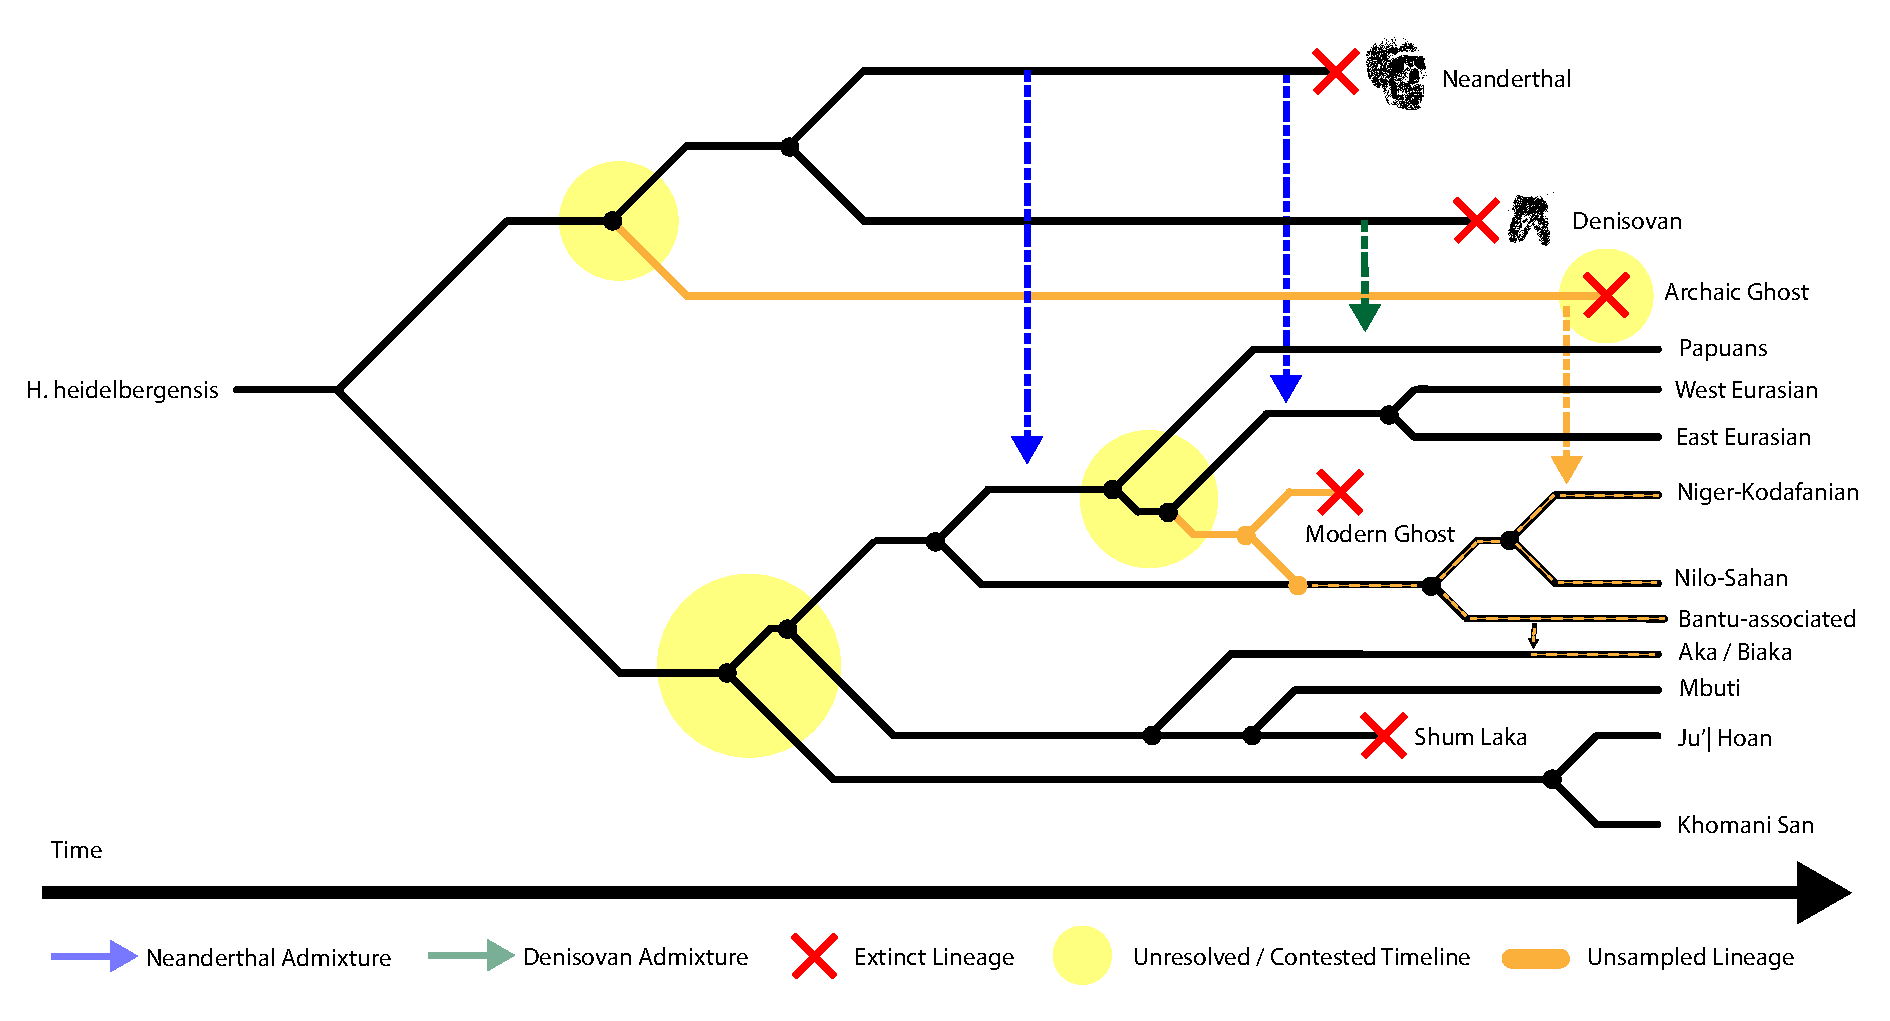
\includegraphics[width=\textwidth]{plot/dem2.pdf}
%	\caption{Proposed Demographic Model. Population splits coloured in yellow are contested. The existance of an archaic ghost lineage which has contributed to Western African populations has been broadly supported in the literature, but the time and order of divergences relative to Neanderthals and Denisovans remains an open question. Until recently, the San peoples were considered to be the most anciently diverged group in Africa, though recent evidence places Central African Hunter Gatherers on a similar timespan, with the addition of a modern ghost population. This existance of this population is additionally supported in the literature and in this article, though the order of divergence is contested. In this article we posit that the ghost diverged from the common ancestor of Eurasians after Papuans had diverged, similar to that suggested in \cite{Malaspinas2016}.}
%	\label{fig_dem}
%\end{figure}

\clearpage

\section{Details of Data Analysis} \label{data-analysis}

\subsection{Inferring population size and migration rates in the Simons Genome Diversity Panel}

This section describes analysis of the Simons Genome Diversity Panel with both {\tt SMCSMC} and MSMC. {\tt SMCSMC} version 1.0.1 was installed from the conda package manager (also found at \url{https://github.com/luntergroup/smcsmc/releases/tag/v1.0.1}), {\tt MSMC2} version 2.1.2 was installed from Github (found at \url{https://github.com/stschiff/msmc2/releases/tag/v2.1.2}) and all analyses were performed on the Oxford Biomedical Research Computation cluster.

We download prephased sequencing data from \url{https://sharehost.hms.harvard.edu/genetics/reich_lab/sgdp/phased_data/} and mask for the strict accessibility mask from the 1000 genomes project. We additionally mask for any sites absent Chimpanzee ancestry due to a known issue with the phasing algorithm \cite{Wang2019a}. We do this masking in {\tt vcftools}. We use {\tt SMCSMC} to convert the sequence data from VCF to seg file format, a format very similar to {\tt MSMC} format. We provide a script to convert from seg file format to {\tt MSMC} file format as well. Unless otherwise noted, the names of individuals used in this paper are the first in their population (i.e. an individual named Yoruban is {\tt S\_Yoruba-1} in the SGDP nomenclature, full list in \ref{samples}).  We select two diploid individuals from each population in Africa  and infer piecewise constant population size and directional migration rates. Specifically, we use the following options for {\tt SMCSMC}:

\begin{verbatim}
smc2 -c -chunks 100 -no_infer_recomb -nsam 4 -I 2 2 2 -mu 1.25e-8 -rho 3e-9 \
    -calibrate_lag 1.0 -EM {EM} -tmax 3.5 -alpha 0.0 -apf 2 -N0 14312 -Np {Np} -VB \
    ${DEMOGRAPHIC_MODEL} -P 133 133016 31*1  -arg -o ${OUTPUT} -segs ${SEGS}
\end{verbatim}

In order, we invoke the use of a QSUB cluster with {\tt -c} and split our analysis into 100 chunk. We do not infer recombination sites along with the demographic model in order to reduce runtime. Four haploid samples, two from each population, are analysed with a mutation rate of 1.25 $\times 10^{-8}$, a recombination rate of 3 $\times 10^{-9}$, and accumulating events for one unit of survival time along the sequence. We use a given number of epochs for parameter units, and bound the upper limits of the trees at 3.5 times the effective population size (set to 14312). We use the look-ahead likelihood to guide the resampling process for a given number of particles {\tt Np} and use variational Bayes in place of the default stochastic expectation maximization algorithm. Parameters are inferred over 31 equally spaced intervals from 133 to 133016 generations in the past, and the sampled posterior ARGs are reported. 

We seed the particle filter with a demographic model of population size and uniform symmetric migration rate, given by the following {\tt scrm} command:

{\small 
\begin{verbatim}
-ej 0.2324 2 1 -eM 0 1 -eN 0.0 6 -eN 0.0037 4.4 -eN 0.0046 3 -eN 0.0058 2 -eN 0.0073 1.4 
-eN 0.0092 0.85 -eN 0.093 1.2 -eN 0.12 1.7 -eN 0.15 2.2 -eN 0.19 2.5 -eN 0.24 2.4 
-eN 0.30 2.0 -eN 0.37 1.7 -eN 0.47 1.4 -eN 0.59 1.2 -eN 0.74 1.0 -eN 0.93 0.91 -eN 1.2 1.6
\end{verbatim}
}

We visualise this demographic model in the POPdemog package in Figure \ref{smc2demog} \cite{Zhou2018}.

Each {\tt SMCSMC} analysis gives a final output file detailing migration and coalescent events, their rates, and their opportunities which denote the total opportunity for an event to occur during a particular epoch. Output files are trimmed to only visualise the final epoch of variational Bayes inference and assessed for convergence. Times and rates are interpreted differently than {\tt scrm} output. Rates are in units of $4N_0$ per generation, while times are given in generations. 

We implement the above in an open source {\tt Snakemake} pipeline at \url{https://github.com/Chris1221/ancient_african_admixture} which also implements a default analysis of MSMC with twenty iterations to converge. Sample size and relative cross-coalescent rates are transformed as described in the documentation using the same parameter values for mutation rate and generation time used for {\tt SMCSMC} analysis. Effective population size and migration estimates for the populations analysed in the SGDP are given in Figures \ref{sgdp_ne} and \ref{sgdp_mig}. MSMC appears to consistently find a higher African $N_e$ in the ancient past until the average estimates across populations stabilises approximately 100kya (Figure \ref{fig:both}a). We expand on a possible reason for this effect in the main text of this article.


Migration during the last 100ky is integrated into a metric we call the inferred migration fraction (IMF). (Figure \ref{sgdp_heatmap}). This is related to the cummulative migration fraction (CMF) as introduced in MSMC-IM \cite{Wang2019a}, except the quantity is integrated in a particular epoch. We use two methods to integrate migration, the first presented in the main text given by $F(t) = e^{- \int_{t=0}^T \rho(t) dt}$. Alternatively, consider $p$ proportion of the population are replaced every generation. Start with 0 individuals from the source $N_{source}$ population in the sink population $N_{sink}$, each generation replace $p$ proportion of the sink population with the source. We track the proportion of the population which are replaced by the source $P$.  

$$ \begin{aligned} P_0 &= 0 \\ P_1 &= pN_{sink} \\ P_2 &= pN_{sink} + p(N_{sink} - pN_{sink}) \\ &= pN_{sink} + pN_{sink}(1-p) \\ P_3 &= pN_{sink} + pN_{sink}(1-p) + p((N_{sink}-pN_{sink}) - p(N_{sink}-pN_{sink})) \\ &= pN_{sink} + pN_{sink}(1-p)+p(N_{sink}(1-p)-pN_{sink}(1-p)) \\ &= pN_{sink}+pN_{sink}(1-p)+pN_{sink}(1-p)(1-p) \\ &\dots \\ P_n &=N_{sink}p(1-p)^n \end{aligned} $$

In practice, both methods give essentially identical proportions for all considered questions. Inferred migration varies across language groups (Figure \ref{migrationplot}, Table \ref{table:sgdp_pairwise}). Afroasiatic groups show high migration from Han and French populations, with a lower proportion deriving from Papuans. Niger-Kordofanian and Nilo-Saharan groups show an intermediate magnitude, between 50 and 60 percent replacement, though also significantly (P < 0.05, two-tailed paired $T$ test) closer to French and Han sources than Papuans. The Khoesan show the lowest migration, consistent with their early diversification from the remainder of African groups and the relative lack of gene-flow from Western African populations \cite{Lipson2019}. This is contrasted with the Mbuti and Biaka, Central African Hunter Gatherer populations who have historically received substantial amounts of gene flow from Western African sources. Both of these populations show the lowest migration in their language group (Table \ref{average_sgdp_migration_table}). 

We track the overall peak of migration rate in different populations (Figure \ref{fig:peaks}a,b). The most common backwards migration peak falls in the epoch between 35--45kya in the Nilo-Saharan and Niger-Kordofanian groups. Forwards migration has an earlier peak, in the epoch spanning 55--70kya. This result must be interpreted in light of the simulation results presented below.  

We model the migration adjusted $N_e$ in Eurasian populations, averaged over African partners, and African populations averaged over Eurasian partners \ref{fig:individual_pop_sizes}. The resulting curves largely represent our prior knowledge of world history, with an early divergence of Papuans consistent with the timing proposed in \cite{Malaspinas2016}, and a second bottleneck of populations inhabiting North America such as the Karitiana and Pima. Because we do not explicitly infer population split times, and have no convenient metric like {\tt MSMC2}, more fine-scale trends are difficult to identify. The African population size models show more discrepancy between populations, including an OoA-like bottleneck in Afroasiatic populations, and a large historical population size in hunter-gatherer groups such as proposed in \cite{Lipson2019}. 



\subsection{Validation in a physically phased subset of the Human Genome Diversity Panel (HGDP)} \label{hgdp_section}

Phased data is not essential for demographic inference using {\tt SMCSMC}; however, the use of phase alongside the look-ahead likelihood allows for more efficient convergence. The Human Genome Diversity Project collected 929 genomes from a diverse collection of human populations \cite{Bergstrom2019}. 36 of these genomes, two each from nine Eurasian and four African populations, were physically phased by use of linked-read sequencing technologies. This resource allows us to validate our inference both in an independent dataset, and evaluate the effect of phasing errors on {\tt SMCSMC} inference.   

To analyse these data, the same {\tt Snakemake} pipeline was used with minor adjustments in wildcard constrains to account for differences in sample names. 120 chunks of the genome were run in parallel for reasons of computational efficiency, while fixed recombination rate and mutation rates were held at the same values as the SGDP analysis, and an identical demographic model was used to initiate the analysis. Three replicates of the analysis were performed to assess the impact of stochastic sampling variation on inference. We infer both effective population size and directional migration in each of these 9x4 comparisons between Eurasian and African populations (Figure \ref{fig:both}a). The resulting inference allows us to verify and validate many observations from the SGDP.

Firstly, we calculate the timing of the migration peak and its magnitude, and find the estimates largely in line with the SGDP inference (Figure \ref{fig:peaks}c,d). For instance, inferred backwards migration in the Yoruban and Biaka populations peak at 40-50kya, while the Mbuti and San show earlier migration peaks around 50-60kya (Figure \ref{fig:peaks}c). The migration rate at the peak shows the same qualitative trends as the SGDP, with the peak in the Yoruban (approximately $2.5\times10^{-4}$) far exceeding the peaks in the Biaka, Mbuti, or San (between $0.1-0.175\times10^{-4}$) (Figure \ref{fig:peaks}d). This replication in the HGDP confirms the presence of a large directional migration in the Late Middle Pleistocene, and demonstrates that statistical errors in phasing the SGDP are not large contributors to the qualitative trends observed. 

We integrate migration between 40--70kya to obtain the inferred IMF for each of the comparisons in the HGDP (\ref{fig:both}b). Differences amung the African populations mirror those in the SGDP, though the proportions are uniformly smaller (main text). However, the migration rates backwards into Africa are apparent in all comparisons, and the order of populations IMF remains the same. Differences between individual Eurasian donor populations are small, and with the exception of the Papuan, insignificant. A discussion of the Papuan comparisons appears in the subsequent section.  

To compare the HGDP inference with the SGDP inference, we construct a set of the SGDP with the same donor populations as the HGDP.



%For the SMCSMC algorithm, the use of phased data is not necessary but does help with efficient convergence by assisting the lookahead-likelihood-guided resampling. Therefore, we do not expect errors made during statistical phasing to significantly impact the inferred parameters. However, to test this, we replicate the above analysis in a physically phased subset of the HGDP downlaoded from \url{ftp://ngs.sanger.ac.uk/production/hgdp/hgdp_wgs.20190516/}. The same {\tt snakemake} pipeline is used as in the analysis of the SGDP data. Data is additionally masked for the filters provided with the data. 

%We first asked if we could replicate the inflated African $N_e$ estimates from the main text in this new, high quality, data set. To do this, we infer effective population size with SMCSMC and MSMC.  The full inference from both algorithms is shown in \ref{fig:hgdp_ne} and \ref{fig:hgdp_mig}. For SMCSMC, we use 10,000 particles and 15 iterations to achieve convergence, with the same recombination and mutation rates as in the SGDP analysis.  The source populations here are more diverse than in the main text, comprising a sample of global diversity including Druze, Han, Karitiana, two Papuans, Pathan, Pima, Sardinians, and Yakut. To obtain a comparable sample from the SGDP, we select populations matching those in the HGDP. We match each of the source and sink populations, and similarly infer their effective population size and migration histories. The full inference is shown in Figure \ref{hgdp_sgdp_ne} and \ref{fig:hgdp_sgdp_mig}.


\subsection{Comparisons between the HGDP and a subset of the SGDP}

Previously, inference in the SGDP has relied on three candidate Eurasian donor populations. However, the physically phased subset of the HGDP provides a higher resolution view into global migration patterns with nine Eurasian populations represented. In order to compare effectively between the inferences made in these two datasets, we find representatives from these nine Eurasian populations in the SGDP dataset and use them as donor populations to the same four African populations (Yoruban, San, Mbuti, and Biaka), effectively recreating the analysis done in the physically phased subset of the HGDP. We select the Khomani San as a representative of the San, and only use one of the Papuan populations in the HGDP to compare (Highlands, as opposed to Sepik), creating the same 8x4 analysis table for both data sets. We infer the effective population sizes and migration rates using both {\tt SMCSMC} and {\tt MSMC}, with analysis details effectively identical to the original comparisons listed above (Figure \ref{fig:hgdp_sgdp}). We average over inferences to visually compare trends between the two datasets, in the same populations and compute the inferred IMF between 40--70kya (Figure \ref{fig:both}).  

In both the HGDP and the SGDP, MSMC estimates of African population size are higher than {\tt SMCSMC} estimates in the ancient past (80 -- 300kya) (Figure \ref{fig:both}a). By modelling directional migration, we are able to account for excess genetic diversity in the ancestral African population in both datasets. Uncertainty in the estimates increases substantially nearer to the present, as would be expected with the {\tt SMCSMC} method. 

We summarise migration from 40--70kya in the HGDP similarly to the SGDP. The total inferred migration is lower in the HGDP than in the SGDP (Figure \ref{fig:both}b). We use this comparison setup to additionally test the differences between Papuan donors and the remainder of Eurasians. We construct a linear model predicting IMF based on an indicator variable of Papuan/not Papuan and the receptor donor population, and find that in both the SGDP and the HGDP, Papuans show approximately 2\% less IMF than other donor populations (Tables \ref{hgdp:papuan_imf}, \ref{sgdp:papuan_imf}). While this difference is small, it is highly significant. However, the demographic scenario causing this difference in inferred IMF is not obvious; it is possible that the Papuan group had begun to diverge from the donating population prior to the admixture event, or alternatively that differences in archaic admixture between Eurasian and Papuan groups make up the difference in affinity. 



However, the qualitative patterns in inferred directional migration rates between populations are similar in both datasets (Figure \ref{fig:both}c). In both datasets, the highest rates are found in the Yorubans, follow by the Biaka, then the Mbuti and San. The MSMC curves are interestingly dissimilar between the different data sets, with a much steeper ascent around the period of our inferred migration in the HGDP than the SGDP. 


\subsection{Samples used in these analyses}

For a list of the identifiers used for the samples listed in this article, see Table \ref{samples}.

\section{Statistical Analysis of Migrated Segments} \label{dstats_section}

We run {\tt SMCSMC} with the {\tt -arg} flag to report the posterior estimate of the ancestral recombination graph. We use this to isolate segments of the African genome where predicted migration events occurred between 50 and 70kya and used these segments to calculate drift statistics. The isolation procedure is implemented in {\tt smcsmc.find\_segments}, and involves sequentially reconstructing marginal trees and keeping track of which contain migration events in a particular epoch. We isolate segments from the marginal trees of all SGDP comparisons. 

\subsection{Length Distribution of Isolated Segments}


 Under the Markovian model of the SMC', the length of admixed tracts $L$ is an exponential process with scale factor $2N (1 - m ) \left( 1 - e^{-T / 2N} \right)$, with a proportion $m$ of the sink population being replaced with the source $T$ generations in the past and an effective population size of $N$ \cite{Marjoram2006,Liang953}. This gives an approximate mean length $\left[ (1 -m)r(T-1) \right]^{-1}$ with recombination rate $r$ in units of Morgans, which is well approximated
by  $(rT)^{-1}(1-m)$ \cite{Racimo2015}; we use this approximation to derive expected distribution of fragment sizes. When analysing populations with {\tt SMCSMC}, we fix the recombination rate at $3 \times 10^{-9}$ uniformly across the genome, in line with that used by {tt MSMC} in simulations \cite[Supp.\ section 7]{Schiffels2014a}.
This value is a conservative underestimate, accounting for the presence of recombination hotspots and {\tt SMCSMC}'s inability to deconvolve recombinations in these areas, effectively underestimating the true $r$.  For estimates of ancestral tract lengths, we use the more universally accepted value of $1 \times 10^{-8}$, equivalent to a one percent chance of a cross-over per megabase and per generation \cite{Dumont2008}. 
%\todo{better reference for recombination rate value}

We take the isolated segments (Figure \ref{fig:length}a) and compute the mean track length (Table \ref{table:lengths}). We use the approximation that the mean segment length should be approximately equal to $((1-m)r(T-1))^{-1}$ to determine that, if the migration happened in one pulse, our empirical distribution would suggest either a recent timing or a very large pulse (Figure \ref{fig:length}b). However, we heavily caveat any interpretation of these data with the fact that they are explicitly generated under a model of a given migration proportion. The fact, therefore, that they are of a consistent length with a large migration is more evidence for the model producing internally-consistent tracts than any external validation of the results in this article. 

The assumption that migration has occurred in a single wave is largely unrealistic. We used expectation maximisation to investigate if a mixture of exponential distributions explained the observed tract lengths better than a single distribution. We found that in some cases, two or three exponential distributions were better supposed by the data, however the differences in log likelihoods was negligible and the support for the different distributions was approximately inversely proportion to their number (data not shown). We found no strong support for multiple waves of migration from this analysis.

\subsection{Individual D statistics}

Here, Yoruba-1 is used as a representative of Western African groups, and used for ascertaining putatively migrated segments. Yoruba-2 is used as a comparison individual from the same populations. In this way, we look for evidence above another individual in the same population of similarity to Eurasians.

We first use $f_3$ statistics to look for evidence of admixture between the African and various Eurasian groups. We calculate $f_3$(Yoruba-1, Eurasian group, Yoruba-2) for Papuans, French, Han Chinese, and the Vindija Neanderthal. We calculate this statistic in all available markers, and additionally for the segments isolated from the three Eurasians separately (Figure \ref{fig:f3}). These statistics show, firstly, that ascertaining in a particular group influences the shared drift with that group. This is exemplified by the non-significant shared drift with Papuans in French and Han ascertained segments. Secondly, these statistic show significant levels ($|Z|>2$) of drift between the test individual and Eurasian populations, while also showing no increase in Neanderthal allele sharing ($f_3$ = 0). To find statistical evidence of admixture, we compute $f_3$(Yoruba-2, Eurasian, Yoruba-1) for the same Eurasian groups. We find statistical evidence for admixture in each of the groups examined, for all ascertainment schemes (Figure \ref{fig:f3_admix}). 



We use $D$ statistics to examine more nuanced scenarios. We find that the two Yorubans share more alleles than other groups in Africa (D(African group, Yoruba-1; Yoruba-2, Chimp) is significantly negative with $|Z|>3$), but the individual of interest is closer to Out of Africa (OoA) groups such as the Han, French, and Papauns (D(OoA, Yoruba-2; Yoruba-1, Chimp) is significantly negative with $|Z|<3$) than to its partner Yoruban (Table \ref{dstats:a1}). This implies that {\tt SMCSMC} has identified segments of the African Genome which are more closely related to OoA populations than to fellow Africans.   


\section{Simulation procedure} \label{simproc}

The ability of {\tt SMCSMC} to recover a back-migration signal is evaluated through simulation. One gigabase of sequence was simulated in {\tt scrm}, and subsequently re-inferred by {\tt SMCSMC}. Migration is parameterised by three factors, magnitude, midpoint, and duration. A scenario is simulated where the midpoint is the center of a block of a given duration which has uniform migration which integrates to a given total proportion replacement over the period. We use the following demographic model for population size throughout all simulations:


The following commands can be used in either {\tt ms} or {\tt SCRM} to specify demographic models. The African population size is given by 

\begin{verbatim}
-en 0.00000000 1 36.9124479 -en 0.00229999 1 14.8978177 -en 0.00299994 1 7.04453213 
-en 0.00391291 1 3.68961222 -en 0.00510371 1 2.06587476 -en 0.00665692 1 1.21617010
-en 0.00868280 1 0.75362392 -en 0.01132521 1 0.49927968 -en 0.01477178 1 0.36258332
-en 0.01926724 1 0.29687253 -en 0.02108190 1 0.28637149 -en 0.02513079 1 0.28071694
-en 0.03277878 1 0.31028768 -en 0.03915210 1 0.36107482 -en 0.04275426 1 0.39815181
-en 0.05576555 1 0.57528787 -en 0.07273654 1 0.88701054 -en 0.09487226 1 1.36014053
-en 0.12374449 1 1.92573639 -en 0.16140334 1 2.36832894 -en 0.21052280 1 2.45284038
-en 0.27459066 1 2.16222564 -en 0.35815613 1 1.71146032 -en 0.46715286 1 1.32388966
-en 0.60932028 1 1.09778746 -en 0.79475315 1 1.04669123 -en 1.03661833 1 1.16969768
-en 1.35208972 1 1.45788656 -en 1.76356769 1 1.80077313 -en 2.30026970 1 1.89942369
\end{verbatim}

While the European population size is given by

\begin{verbatim}
-en 0.00000000 2 1.14422216 -en 0.00229999 2 1.14422216 -en 0.00299994 2 1.14422216
-en 0.00391291 2 1.14422216 -en 0.00510371 2 1.14422216 -en 0.00665692 2 1.14422216
-en 0.00868280 2 1.14422216 -en 0.01132521 2 1.14422216 -en 0.01477178 2 1.14422216
-en 0.01926724 2 1.14422216 -en 0.02108190 2 1.14422216 -en 0.02513079 2 1.14422216
-en 0.03277878 2 1.14422216 -en 0.03915210 2 1.14422216 -en 0.04275426 2 1.14422216
-en 0.05576555 2 1.14422216 -en 0.07273654 2 1.14422216 -en 0.09487226 2 1.36014053
-en 0.12374449 2 1.92573639 -en 0.16140334 2 2.36832894 -en 0.21052280 2 2.45284038 
-en 0.27459066 2 2.16222564 -en 0.35815613 2 1.71146032 -en 0.46715286 2 1.32388966
-en 0.60932028 2 1.09778746 -en 0.79475315 2 1.04669123 -en 1.03661833 2 1.16969768
-en 1.35208972 2 1.45788656 -en 1.76356769 2 1.80077313 -en 2.30026970 2 1.89942369
\end{verbatim}

Times are in units of $4N_0g$ while population sizes are in units of $N_0$. For $g=29, N_0 = 14312$, the demographic model is as shown in Figure \ref{fig:dem}.  

The demographic model which we have assumed for both population's effective sizes has been shown to recapitulate similar inference to real data (data not shown). The migration parameter must be initiated at a given magnitude; further back in time, the particle filter is less able to identify lineage's true populations, and the inference of migration rates becomes essential uniform. Thus, we see a ``drop-off'' effect, where in the ancient past, the inference remains at the initiation value, and as more certainty about different histories is obtained, the migration values recapitulate real information. Thus the choice of an appropriate parameter for the initial migration rate is a crucial step in {\tt SMCSMC} analysis, and here we chose to arrive at this value through simulation.

We simulate back-migration scenarios of varying total migration proportions from 0 (no migration) up to 60\% population replacement.For each simulation, we initiate the particle filter at either 0, 1, or 5 4$N_0$ proportion replaced per generation (which are the units used internally by {\tt scrm} and {\tt ms} for simulation).  {\tt SMCSMC} is then used to infer effective population size and migration histories in five iterations with 5000 particles. As a cautionary note, these simulations are almost certainly not fully converged, and are used as an indication of power. Their power, theoretically, approaches 1, as particle filters asymptotically exactly approach the true posterior distribution. However, these low resolution attempts are indicative of a ``quick'' overview of the abilities of the algorithm. With 600 cores available, each of the cases (forward, backward, or bidirectional) was able to run in approximately 20 hours. 

Generally, beginning with a higher migration rate seems to recover a higher proportion of the simulated migration. However, as in the case of a 60\% replacement simulated 40kya, beginning with 5 4$N_0$ rather than 1 4$N_0$ recovers similar proportions of backwards migration (0.502 vs 0.52) yet the higher migration rate finds 0.301 Eurasian migration rather than 0.195. The higher initial migration rates thus slightly reduce power (though, not in all cases, and for fully converged solutions, we would expect both proportions to be similar up to noise) while additionally finding an increased migration in the opposite direction.  Beginning with a zero rate leads to highly unstable estimates of the migration rate and effective population size, and we exclude it from our analysis.

We select a more comprehensive set of initiation parameters and particle values and use them to analyze a Yoruban and French individual from SGDP (Fig \ref{init_yri}). The effect of the initial migration rate seems relatively consistent for low values (0.5 - 2.0),while an increasingly small migration peak is seen for higher initial magnitudes 4.0 - 10.0. Again, beginning with an initial rate of zero tends to lead to highly unstable estimates of effective population size and migration rates. For the remainder of the analyses in this article, we choose to use an initial rate of 1.0. 



%\begin{figure}
%	\centering
%	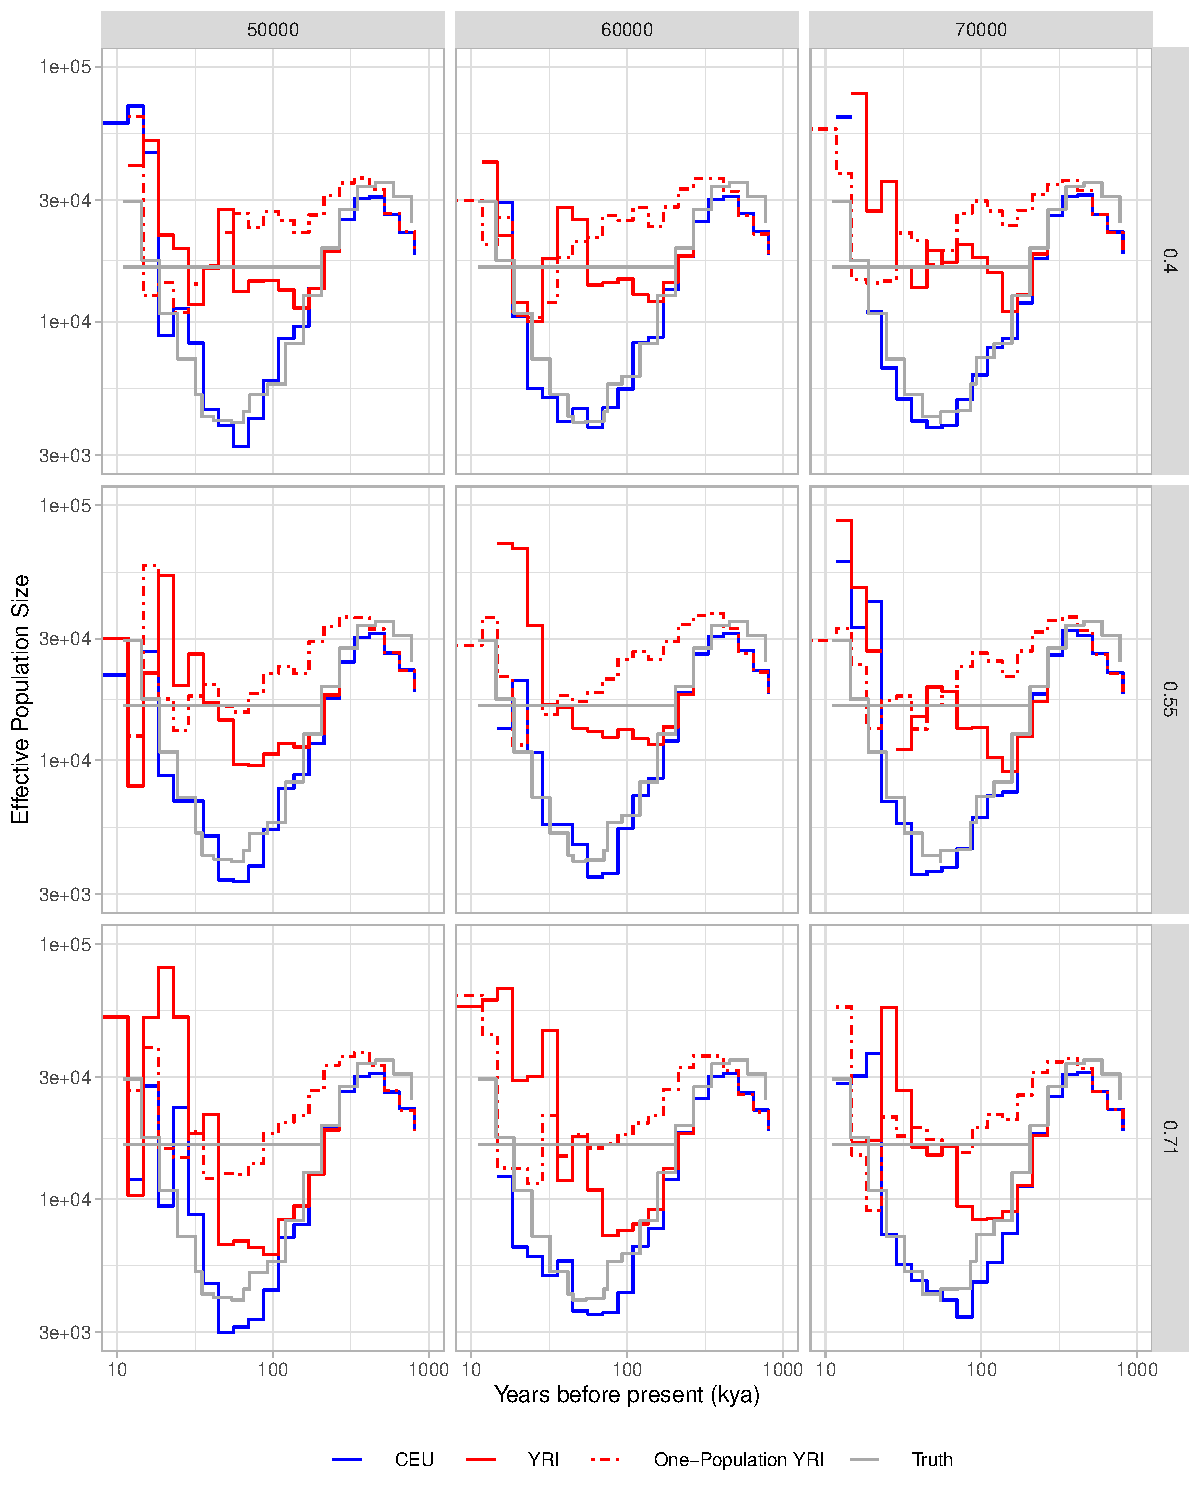
\includegraphics[width=0.5\textwidth]{plot/old_all_li_durbin.pdf}
%	\caption{Simulated directional migration from effective ``African'' to ``Eurasian'' populations. For this figure, duration of the migration was fixed at 10ky. Simulations performed in {\tt scrm} with one gigabase of sequence. Inference performed in {\tt SMCSMC} with five iterations of variational Bayes and 5000 particles.}
%	\label{nesims_10ky}
%\end{figure}

% old intro

%The early population structure of anatomically modern humans (AMHs) in Africa and their eventual migration into the Eurasian continent have shaped global patterns of genetic variation \cite{Pagani2016, Nielsen2017a}. However, little is known about population structure within Africa prior to the expansion of agriculturalists and pastoral groups \cite{Busby2016, Patin2017}. Recent evidence from the handful of successfully sequenced ancient African genomes hint at large-scale population movements and admixture from multiple highly divergent, extinct populations, with complex affinities to current groups \cite{Skoglund2018, Lipson2019, GallegoLlorente2015a}. The majority of structure in the continent is derived from events in the Holocene, including the spread of Bantu languages from Western Central Africa both East and South, as well as admixture from pastoralists its in the Near East and Western Eurasia \cite{Busby2016}. Eastern Africans are the most closely related group to the ancestral Out of Africa migrants, though they show particularly high levels of ancestry related to neolithic populations from Iran and the Levant consistent with multiple waves of back-migration in the Holocene \cite{Skoglund2017}.  Evidence for recent admixture from Eurasian sources is well established, however the lack of ancient African DNA from the Pleistocene has confounded efforts to uncover interactions between the earliest inhabitants of the continent. While the migration event associated with establishing current global population structure has been confidently dated between 60-80kya, Central and South African hunter gatherers such as the Mbuti and KhoeSan (without implying linguistic unity, defined as southern African hunter gatherers who speak non-Bantu languages which include a click consonant) may have diverged from other groups 200-250 thousand years ago (kya) \cite{Lipson2019, Schlebusch2017}. In the intervening millennia, fossils identified as AMH have been found in China about 80-120kya, Sumatra about 63-73kya, and artifacts from Australia 65kya \cite{Clarkson2017, Liu2015, Westaway2017}. Support for multiple migrations across Eurasia additionally comes from climate science, where four distinct periods of warming may have provided vegetated migration routes out of Africa (OoA) as early as 120kya \cite{Timmermann2016}. The extent of contributions to modern day populations from ``ghost'' populations is unknown, though controversially suggested in Australasia and South East Asia \cite{Malaspinas2016, Mallick2016, Pagani2016, Rasmussen2011, Skoglund2015} and Africa  \cite{Durvasula2019, Speidel2019, Lipson2019, Hammer2011, Plagnol2006, Ragsdale2019}. To a large degree, the fate of these anciently diverged populations and their contributions, if any, to modern day populations remains an open question. Here, we apply a recently developed particle filter using the sequentially Markovian approximation of the coalescent with recombination to dissect historical directional migration in Africa \cite{Henderson2018}. 

%\todo[inline]{Question: Do you think that we need a review of other methods here? Do we need to defend our choice to use smcsmc?}

%Little is known about population structure within the African continent Current evidence mostly supports an early diversification of both Central and South African hunter gatherers, though the order is not yet resolved, possibly up to 200-250kya. \cite{Lipson2019,Schlebusch2017, Skoglund2017} The divergence between African and Out of Africa (OoA) lineages has been robustly dated to between 60 and 80kya, supported by both whole genome demographic inference and mtDNA phylogeography \cite{Lipson2019,Soares2012}. In the intervening millennia, archaeological evidence supports AMHs inhabiting sites in China, Australia, and Sumatra before the main OoA event \cite{Clarkson2017, Liu2015, Westaway2017}. The fate of these earlier migrants and their contribution to modern day populations remain an open question. 

%Unsampled populations, sometimes referred to as ``ghost'' populations, have been suggested to contribute to several global populations, most notably and controversially in Australasia and South East Asia . However, recent evidence points towards large unexplained patterns of admixture from both ancient and modern populations to several groups in Africa \cite{Durvasula2019, Lipson2019, Skoglund2017, Hammer2011, Plagnol2006, Ragsdale2019}. Support for these admixture events mainly derives from inference under approximations of the coalescent with recombination, analysing the site frequency spectrum, and fitting expectations of drift statistics to observed quantities. However, to date an understanding of the magnitude and timing of these migration events has been confounded by a lack of appropriate statistical methods for inferring directional migration over a wide range of time. 

%Approximating the coalescent with recombination with a Markovian process along the genome has provided a tractable framework for the inference of effective population size \cite{McVean2005}. Recent applications have adopted the sequentially Markovian coalescent (SMC) and its derivatives for inference in up to eight haploid individuals in methods such as the pairwise and multiple SMC (PSMC and MSMC) \cite{Li2011, Schiffels2014}. MSMC additionally infers a cross-population coalescent rate, which can be scaled to reflect relative symmetrical gene flow. Both methods estimate $N_e$ as the scaled inverse of the coalescent rate, a quantity which is equivalent to effective population size in panmictic populations but not in the presence of structure \cite{Chikhi2018}. Here, we use a newly developed particle filter to simultaneously estimate both $N_e$ and directional migration in up to eight haploid individuals, and explore population structure in the ancient past. A combination of importance sampling and a resampling process guided by a novel lookahead-likelihood samples from the posterior distribution of piecewise constant geneological trees collectively called the ancestral recombination graph (ARG). Variational Bayesian inference is used to estimate, in theory any demographic parameter which admits simulation along the sequence, but in practice effective population size and directional migration rates.  



% old results
%One individual was selected from each of the African populations in the Simons Genome Diversity Panel and their effective population size was modelled along with three seperate partner populations (French, Han Chinese, and Papuan) using both {\tt SMCSMC} and MSMC (Figure \ref{neplot}). Directional migration rates between the African and Eurasian populations are simultaneously estimated; the converged parameter estimates represent the most likely set of piecewise constant parameter values. We choose to infer parameter values over 31 epochs equally spaced on the log scale. The inference of population size with MSMC and {\tt SMCSMC} is mostly consistent, especially for the estimation of the Eurasian $N_e$ (blue in Figure \ref{neplot}). Both algorithms identify a clear bottleneck and subsequent expansion associated with the Out of Africa event. However, the estimation of African population size differs. In the ancient past, prior to the OoA event, MSMC identifies an early split between the two populations, followed by a transient increase in the African $N_e$ up to an average of approximately 40,000 individuals before coming back down to a stable estimate (red in Figure \ref{neplot}, detail in Figure \ref{averages}). This contrasts with the inference from {\tt SMCSMC}. In all populations, there is no inflation in the African $N_e$ relative to the Eurasian one prior to population divergence, and the split times are additionally delayed, bringing them more in line with current estimates. A smaller ancestral African population size is inferred in each individual averaged over Eurasian donor (Figure \ref{averages}). We suspect that the differences in population size inference may be due to {\tt SMCSMC} simultaneously accounting for directional migration. To test whether systematic differences in the inference methods may be responsible, a single population model is fit to two Yoruban genomes. When no migration parameters are fit, {\tt SMCSMC} and MSMC infer very similar histories (green in Figure \ref{neplot}). To verify that systematic errors in the statistical phasing of the SGDP were not confounding inference, we performed the same analysis on 32 individuals from the Human Genome Diversity Panel whose genomes have been physically phased (Supplemental Section \ref{hgdp_section}). All trends identified in the SGDP are additionally present in the physically phased HGDP.   

%\todo[inline]{I haven't made plots for the HGDP analysis yet becuase the MSMC runs haven't finished.}

%A variety of demographic scenarios were simulated in {\tt scrm} to investigate the role of migration in population size inference. The timing of the migration, its duration, as well as the total proportion of the sink population replaced are varied systematically. Population size was inferred under a two island model with migration, performed similarly to the analysis of real data above. Additionally, the ``African'' genome in the analysis is isolated and modelled alone in a one-population analysis. A skeleton of Eurasian and African population size through time, given in Supplemental \ref{simproc}, is used as the truth in the simulations. Systematic underestimation of the African $N_e$ is found in the two-population analysis, while the $N_e$ is systematically inflated during the migration event and prior to population split in the single-population analysis (Figure \ref{sim}).  

%Examining the migration rates inferred by {\tt SMCSMC} supports this hypothesis. In all populations studied, migration from Eurasia to Africa is higher than the reverse (Figure \ref{migrationplot}a). The choice of Out of Africa population significantly impacts the amount of migration inferred (Figure \ref{averages_of_sgdp}). In general, and in each specific language family, Papuans significantly contributed approximately 5 percent less (individual comparisons shown in Figure \ref{averages_of_sgdp}) to the ancestral African population than did Han and French, which were statistically indistinguishable in all language groups (P $>$ 0.05, two-tailed paired $T$ test). For convenience, the following values are given for Han Chinese comparison, though all comparison averages are available in Table \ref{average_sgdp_migration_table}. Afroasiatic populations, which are known to have experienced Eurasian admixture during the Holocene, show up to a 72.1\ $\pm$ 2.9 replacement by Eurasian sources, though they contributed more to Western European (35.1 $\pm$ 9.2 percent contribution to French) than to Eastern Eurasian (24.1 $\pm$ 5.5 percent contribution to Han Chinese) populations. Nilo-Saharan and Niger-Kordofanian  populations show similar levels of migration, at 59.5 $\pm$ 7.9 and 51.4 $\pm$ 5.9 percent respectively. Khoesan show the least migration, averaging only 30.4 $\pm$ 0.5 proportion replaced over the last 100ky. MSMC inference clearly shows a different relatively cross-coalescent curve between Yoruban and San populations, which supports different migration histories for the two populations (Figure \ref{migrationplot}b,c). Compared to the MSMC inference, {\tt SMCSMC} finds coalescent events across populations more recently, though a direct comparison between the magnitudes is infeasible. 

%Without an understanding of the true demography, various demographic models are explored via simulation. {\tt scrm} is once again used to simulate directional migration in either direction and bidirectionally. The timing of the migration, its duration, and its magnitude are varied systematically. We plot the full inferred migration and effective population size histories of the backward, forward, and bidirectional cases in Figures \ref{fig:backsim}, \ref{fig:bisim}, and \ref{fig:fwdsim}. Integrated migration proportions are shown in Figure \ref{fig:intsim}. The inference of population size is generally consistent, up to noise and the low resolution of the inference. African population size estimation is systematically lower for higher magnitudes of simulated migration. Given that the magnitudes being simulated are somewhat unrealistic, and the simulations involve pure migration in one direction at a constant rate over a long period, this is not unexpected. No other remarkable trends can be seen in the inference of the effective population size. Empirically, {\tt SMCSMC} has more power to detect migration in the more recent past, recovering up to 99\% of the total simulated migration for a moderate event 40kya, while it can only recover 46\% of the same event 70kya (Figure \ref{fig:intsim}). {\tt SMCSMC} also has less power to detect Eurasian migration than African migration, recovering 54\% and 22\% for the same events 40 and 70kya. 
 
%We use the estimate of the posterior distribution generated with the {\tt SMCSMC} particle filter and isolate the individual trees which contain migration events from Eurasians to Africans between 50 and 75 kya on a sample-by-sample basis. We construct migration segments from these trees, and use these segments to calculate drift statistics. When we isolate segments in one particular Yoruban, we find that more alleles are shared with OoA populations (Han, French), than with a comparable Yoruban. In the same segment, more alleles are shared between the Yoruban populations than with other African populations. We find that both Yorubans share more alleles with OoA populations than do a Khoesan group, but the magnitude of sharing is higher in the individual used to isolate segments. In this individual, more alleles are shared with OoA populations ($D$(Yoruban-1, Yoruban-2, OoA, Chimp)). However, we find no evidence of shared alleles between this Yoruban and Neanderthals. Additionally, we do not find more shared drift with the Vindija Neanderthal than the Altai, as would be expected if introgression had occured from Euroasian sources \cite{Prufer2017}. We use the following experiment to examine if $D$ statistics are, in general, inflated in the individual from which the segments were ascertained. For each African individual $A$, we find a partner in the same population $A_p$ and calculate D(A, A$_p$, Y, Chimp) for a panel of global populations Y from the Reich Lab genotype dataset. $D$ statistics which significantly differ from zero indicate evidence for admixture, with the sign indicating the direction. We compare these ``segment statistics'' against statistics calculated for all available markers, which, up to noise, should be equal to zero. The segments of the African genomes isolated by {\tt SMCSMC} show higher drift with global populations, both modern and ancient (Figure \ref{dstats}a). Overall, statistics are higher in the segments, which is consistent with our expectations, given that {\tt SMCSMC} effectively isolates parts of the African genome that appear to be more Eurasian (Figure \ref{dstats}b,c). We look specifically at the samples in the Reich dataset which have been dated to the Paleolithic (>11.7kya) and find no sample which is consistently closer to all segments. However, we find that Denisovan and Neanderthal drift statistics are not inflated in the segments (Figure \ref{dstats}d). 

%\todo[inline]{I want to have an actual run with the Vindija to confirm this. Just in case the weird migration initiation was blinding us before}



\end{document}
